%#MAKEINDEX /usr/texbin/makeindex main
\documentclass[a4paper,11pt,twoside]{report}
%%\usepackage{program}
\usepackage{ascmac}
\usepackage[dvipdfmx]{graphicx}  % for EPS and PDF 
\usepackage{url}
\usepackage{fancyvrb}
\usepackage{makeidx}
\usepackage{here}
%\usepackage[sectionbib]{chapterbib}

\usepackage{vruler}  %% if vertical ruler (line number) is needed

%\usepackage[dvipdfm,bookmarkstype=toc,colorlinks=true,urlcolor=black,%
%    linkcolor=black,citecolor=black,linktocpage=true,bookmarks=false]{hyperref}
%\usepackage[dvipdfm,bookmarkstype=toc,colorlinks=true,urlcolor=black,%
%    linkcolor=black,citecolor=black,bookmarks=false]{hyperref}
\usepackage[dvipdfm,bookmarkstype=toc,urlcolor=black,%
    linkcolor=black,citecolor=black,bookmarks=false]{hyperref}

\setcounter{secnumdepth}{4}
\setcounter{totalnumber}{6}
\usepackage{fancyhdr}


\hoffset=0cm
\oddsidemargin=0cm
\evensidemargin=0cm
\textwidth=16cm
%\topmargin=-1.5cm
\topmargin=-1cm
\voffset=0cm
\textheight=24cm

\long\def\comment#1{}
\def\progenv{\baselineskip=10pt\tt\progspecial{`}\parindent=0.3cm}
\def\shellenv{\baselineskip=10pt\tt\progspecial{`}\parindent=0.3cm\nolineno}

%%\renewcommand{\topfraction}{0.85}
%%\renewcommand{\textfraction}{0.1}
%%\renewcommand{\floatpagefraction}{0.75}

\renewcommand{\topfraction}{.99}
\renewcommand{\bottomfraction}{.99}

\def\openb{{\it [}}
\def\closeb{{\it ]}}
%\def\openp{{\tt (}}
%\def\closep{{\tt )}}

\def\DAG{$^\dagger$}
\def\DDAG{$^\ddagger$}

\def\XMP{XcalableMP}
\def\OMP{OpenMP}
\def\HPF{HPF}
\def\CAF{Co-array Fortran}
\def\MPI{MPI}
\def\Fort{Fortran}
\def\C{C}
\def\XMPF{XcalableMP Fortran}
\def\XMPC{XcalableMP C}

\def\Directive#1{{\tt #1}\index{#1@{\tt #1}}\index{Directive!#1@{\tt #1}}}

%\def\Syntax#1{\index{{\tt #1}}\index{Syntax!{\tt #1}}}
\def\Syntax#1{\index{Syntax!#1@{\tt #1}}}

\def\Term#1{{#1}\index{#1}}

%\def\Example#1{\index{#1}\index{Example!{\tt #1}}}
\def\Example#1{\index{Example!#1@{\tt #1}}}

\def\Intrinsic#1{\index{#1@{\tt #1}}\index{Intrinsic and Library Procedures!#1@{\tt #1}}}

\def\NULL{{\tt NULL}}

\def\PROG#1{{\tt #1}\index{\tt #1}\index{Command!#1}}
\def\FUNC#1{{\tt #1()}\index{\tt #1}\index{Example Function!#1}}
\def\LPROG#1{{\tt #1}\index{\tt #1}\index{Linux Command!#1}}
\def\LFUNC#1{{\tt #1()}\index{\tt #1}\index{Linux Function!#1}}
\def\MFUNC#1{{\tt #1()}\index{\tt #1}\index{Myrinet/MX Function!#1}}
\def\SFUNC#1{{\tt #1()}\index{\tt #1}\index{Sample Code!#1}}
\def\STRUCT#1{{\tt #1}\index{\tt #1}\index{Struct!#1}}
\def\VAR#1{{\tt #1}\index{\tt #1}\index{Variable!#1}}
\def\ARG#1{{\tt #1}\index{\tt #1}\index{Variable!#1}}
\def\MACRO#1{{\tt #1}\index{\tt #1}\index{Macro!#1}}
\def\ERRNO#1{{\tt #1}\index{\tt #1}\index{ERRNO!#1}}
\def\SIGNAL#1{{\tt #1}\index{\tt #1}\index{Signal!#1}}
\def\FILE#1{{\tt #1}\index{\tt #1}\index{File!#1}}
\def\ENV#1{{\tt #1}\index{\tt #1}\index{Environment Variable!#1}}
\def\INDEX#1{#1\index{#1}}
\def\OPTION#1{{\tt #1}\index{Command Option!#1}}
\def\TERM#1{\underline{#1}\index{#1}}
\def\CTRL#1{{\tt $^\wedge$#1}}

\def\phrule{\vspace{0.2cm}\hrule\vspace{0.05cm}\hrule}
\def\qhrule{\vspace{0.2cm}\hrule}

\def\dhrule{\hrule\vspace{0.05cm}\hrule}

\def\bsquare{\rule[-2pt]{5pt}{10pt}}

\newcommand\gio{{\tt global\_io }}
\newcommand\mio{{\tt master\_io }}

\newcommand{\mytextcolor}[2]{\textcolor{#1}{#2}}
\newcommand{\mycolor}[1]{\color{#1}}

\newenvironment{point}[1]{\vspace*{0.3cm}\begin{itembox}{#1}}{\end{itembox}\vspace*{0.3cm}}

\newenvironment{note}[1]{\vspace*{0.3cm}\begin{itembox}{Note on #1}}{\end{itembox}\vspace*{0.3cm}}

\newenvironment{issue}[1]{\vspace*{0.3cm}\begin{itembox}{Issues on #1}}{\end{itembox}\vspace*{0.3cm}}

\newenvironment{errors}{\vspace*{0.3cm}\begin{tabular}{ll}\multicolumn{2}{l}{\bf Return Values}\\}{\end{tabular}\vspace*{0.3cm}}

\newenvironment{mytable}[3]{\begin{table}[ht]\caption{#1}\label{#2}\vspace*{-0.3cm}\begin{center}\begin{tabular}{#3}}{\end{tabular}\end{center}\end{table}}

\newenvironment{myfigure}{\begin{figure}[ht]\begin{center}}{\end{center}\end{figure}}

\DefineVerbatimEnvironment{Fexample}{Verbatim}{numbers=left,numbersep=3pt,stepnumber=5,frame=single,label=\Fort}

\DefineVerbatimEnvironment{FexampleR}{Verbatim}{numbers=right,numbersep=3pt,stepnumber=5,frame=single,label=\Fort}

\DefineVerbatimEnvironment{Cexample}{Verbatim}{numbers=left,numbersep=3pt,stepnumber=5,frame=single,label=\C}

\DefineVerbatimEnvironment{CexampleR}{Verbatim}{numbers=right,numbersep=3pt,stepnumber=5,frame=single,label=\C}

\DefineVerbatimEnvironment{XFexample}{Verbatim}{numbers=left,numbersep=3pt,stepnumber=5,frame=single,label=\XMPF}

\DefineVerbatimEnvironment{XFexampleR}{Verbatim}{numbers=right,numbersep=3pt,stepnumber=5,frame=single,label=\XMPF}

\DefineVerbatimEnvironment{XCexample}{Verbatim}{numbers=left,numbersep=3pt,stepnumber=5,frame=single,label=\XMPC}

\DefineVerbatimEnvironment{XCexampleR}{Verbatim}{numbers=right,numbersep=3pt,stepnumber=5,frame=single,label=\XMPC}

%% End of Preemble

\title{{\Huge XcalableMP}\\
$\langle${\it ex-scalable-em-p}$\rangle$\\
Language Specification\\
%Application Program Interface\\
\vspace{2cm}
Version 1.2\\}
%DRAFT 0.7}
\author{
\Large XcalableMP Specification Working Group\\
}
\date{\vspace{4cm}\Large November, 2013}

\makeindex

\begin{document}
\maketitle

Copyright \copyright 2008-2013 {\XMP} Specification Working Group.
Permission to copy without fee all or part of this material is granted,
provided the {\XMP} Specification Working Group copyright notice and the
title of this document appear. Notice is given that copying is by permission
of {\XMP} Specification Working Group.

\pagenumbering{roman}
\tableofcontents
\listoffigures
\listoftables
%%%%\listoftables

\chapter*{Acknowledgment}

The specification of {\XMP} is designed by the {\XMP} Specification
Working Group, which consists of the following members from academia,
research laboratories, and industries.

\begin{itemize}
\setlength{\itemsep}{-1mm}
\item Tatsuya Abe        \dotfill \ RIKEN
\item Tokuro Anzaki      \dotfill \ Hitachi
\item Taisuke Boku       \dotfill \ University of Tsukuba
\item Toshio Endo        \dotfill \ TITECH
\item Yoshinari Fukui    \dotfill \ JAMSTEC
\item Yasuharu Hayashi   \dotfill \ NEC
\item Atsushi Hori       \dotfill \ RIKEN
\item Kohichiro Hotta    \dotfill \ Fujitsu
\item Hidetoshi Iwashita \dotfill \ Fujitsu
\item Susumu Komae       \dotfill \ AXE
\item Atsushi Kubota     \dotfill \ Hiroshima City University
\item Jinpil Lee         \dotfill \ University of Tsukuba
\item Toshiyuki Maeda    \dotfill \ RIKEN
\item Motohiko Matsuda   \dotfill \ RIKEN
\item Yuichi Matsuo      \dotfill \ JAXA
\item Kazuo Minami       \dotfill \ RIKEN
\item Shoji Morita       \dotfill \ AXE
\item Hitoshi Murai      \dotfill \ RIKEN
\item Kengo Nakajima     \dotfill \ University of Tokyo
\item Takashi Nakamura   \dotfill \ JAXA
\item Tomotake Nakamura  \dotfill \ RIKEN
\item Mamoru Nakano      \dotfill \ CRAY
\item Masahiro Nakao     \dotfill \ University of Tsukuba
\item Takeshi Nanri      \dotfill \ Kyusyu University
\item Kiyoshi Negishi    \dotfill \ Hitachi
\item Satoshi Ohshima    \dotfill \ University of Tokyo
\item Yasuo Okabe        \dotfill \ Kyoto University
\item Hitoshi Sakagami   \dotfill \ NIFS
\item Tomoko Sakari      \dotfill \ Fujitsu
\item Shoich Sakon       \dotfill \ NEC
\item Mitsuhisa Sato     \dotfill \ University of Tsukuba
\item Taizo Shimizu      \dotfill \ PC Cluster Consortium
\item Takenori Shimosaka \dotfill \ RIKEN
\item Yoshihisa Shizawa  \dotfill \ RIST
\item Shozo Takeoka      \dotfill \ AXE
\item Hitoshi Uehara     \dotfill \ JAMSTEC
\item Masahiro Yasugi    \dotfill \ Kyoto University
\item Mitsuo Yokokawa    \dotfill \ RIKEN
\end{itemize}

This work was supported by ``Seamless and Highly-productive Parallel
Programming Environment for High-performance Computing'' project funded
by Ministry of Education, Culture, Sports, Science and Technology,
Japan, and is supported by PC Cluster Consortium.

\newpage
\mbox{}\newpage

\pagestyle{fancy}
\fancyhead{} % clear all header fields
\fancyhead[RE]{\leftmark}
\fancyhead[LO]{\rightmark}
\fancyhead[LE,RO]{\thepage}
\fancyfoot{} % clear all footer fields
\renewcommand{\headrulewidth}{0pt}
\renewcommand{\footrulewidth}{0pt}


\setvruler[][][][3][0]
\chapter{Introduction}
\pagenumbering{arabic}
\setcounter{page}{1}

This document specifies a collection of compiler
directives, i.e., runtime library routines that can be used to specify
distributed-memory parallel programming in \C and \Fort
programs. These compiler directives define the specifications of the \XMP Application
Program Interface (\XMP API). These specifications provide a
model of parallel programming for distributed memory multiprocessor
systems. The directives extend the \C and \Fort base languages to
describe distributed memory parallel programs.

\section{Scope}

\XMP API
is used to explicitly specify the action to be taken by the compiler
and the runtime system to execute the parallel program in a distributed
memory system. \XMP-compliant implementations are not required
to check for invalid local data access, data conflicts, racing
conditions, or deadlock. The \XMP is defined by following items:

\begin{itemize}
\item A set of directives
\item Minimum language extension on base languages (\C and \Fort)
\item Runtime libraries
\item Environment Variables
\end{itemize}

\section{Features of \XMP}

The features of \XMP are summarized as follows:

\begin{description}
\item {\bf Language extensions} for familiar languages, such as \C and FORTRAN,
  that can reduce code-rewriting and educational costs.
\item \XMP supports typical parallelization based on the {\bf data parallel
  paradigm} and work sharing under {\it global view} and enables
  parallelization of the original sequential code with minimal
  modification using simple {\bf directives}, such as \OMP. 
\item \XMP also includes a CAF-like Partitioned
Global Address Space (PGAS) feature as {\it local-view} programming. 
\item {\bf Explicit communication and synchronization}. All actions
  are taken by directives for being ``easy-to-understand'' for
  performance-aware programming 
\item For flexibility and extensibility, the execution model
allows {\bf combination with explicit \MPI coding} for more complicated
and tuned parallel codes and libraries. 
\item For multi-core and SMP clusters,
{\bf \OMP directives can be combined} into \XMP for thread
programming inside each node as a hybrid programming
model.
\end{description}

\XMP is being designed based on experience obtained in the development of HPF, Fujitsu XPF
(VPP FORTRAN), and OpenMPD.  

\chapter{Overview of the \XMP model and language}

\section{Hardware model and execution model}

The target of \XMP is a distributed memory system
(Figure \ref{fig1}). Each computation node, which may have
several cores sharing main 
memory, has its own local memory, and each node is connected via
network. Each node can access and modify its local memory directly
and can access the memory on other nodes via communication. However, it is assumed that accessing remote memory is much slower than
accessing local memory.

The basic execution model of
\XMP is a Single Program Multiple Data (SPMD) model on
distributed memory. In each node, a program starts from the same main
routine. An \XMP program begins as a single thread of execution
in each node. 

When the thread encounters \XMP directives,
synchronization and communication occurs between nodes. In other words,
no synchronization or communications occur without directives. In
this case, the program performs duplicate execution of the same program
on local memory in each node.

\OMP API can be used in order to
make use of multicores in a node. In this specification, we define
actions only when \XMP directives are executed one thread at a time .

\begin{myfigure}
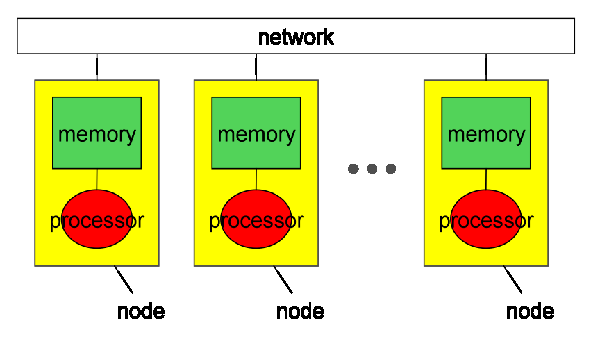
\includegraphics[width=12cm]{figs/Fig1.eps}
  \caption{Hardware Model}\label{fig1}
\end{myfigure}

By default, data declared in the program are allocated in each node and are referenced
locally by threads executed in the node. 

\XMP supports two models of data viewing: the global-view programming model and the local-view programming model. In the local-view programming model, accesses to data
in remote nodes is performed explicitly by language extension for get/put
operations on remote nodes with the node number of the target nodes, while
reference to local data is executed implicitly. 

In contrast to
a local-view programming model, a global-view programming model is
a model in which programmers express their algorithm and data structure in their entirety, mapping them to the node set. The programmers describe the
data distribution and the work mapping in order to express how to distribute
data and share the workload among nodes. The variables in the global-view
programming model appear as a shared memory spanning the nodes.

\section{Global-view programming model}

The global-view
programming model is useful when, starting from sequential version of
the program, the programmer parallelizes the program in the data-parallel model by
adding directives incrementally with minimum modification. In the
global-view programming model, the programmer describes the data
distribution of the data shared among the nodes by data distribution
directives. {\tt loop} iteratively construct maps to the node where the 
computed data is located. Global-view communication directives are
used for synchronization between nodes, to maintain the consistency of the shadow
area, and to move part of the distributed data globally. Note 
that the programmer must perform all computations
that require data reference locally by any appropriate directives. 

In many cases, the
\XMP program using the global-view programming model is based on a sequential
program and can produce the same results independent of the
number of computation nodes (Figure \ref{fig2}). The
global view provides a 
programming model in which computation and data are distributed onto
computation nodes.

There are three groups of directives for the
global-view programming model. Since these directives can be ignored as a
comment by the compilers of base languages (\C and \Fort), an
\XMP program derived from a sequential program can preserve the
integrity of the original program when the program is run sequentially. 

\subsubsection*{Data Mapping}
Specify the data distribution and mapping to nodes (partially
inherited from HPF).

\subsubsection*{Work Mapping (Parallelization)}
Assign tasks to nodes. The {\tt loop} construct maps each iteration to
nodes containing the referenced elements, and the Task construct
executes each task in parallel in different node sets.

\subsubsection*{Communication and Synchronization}
Describe how to communicate and synchronize with the other compute
nodes. In \XMP, inter-node communication must be described
explicitly. The compiler guarantees that communication takes place
only if communication is explicitly specified.

\begin{myfigure}
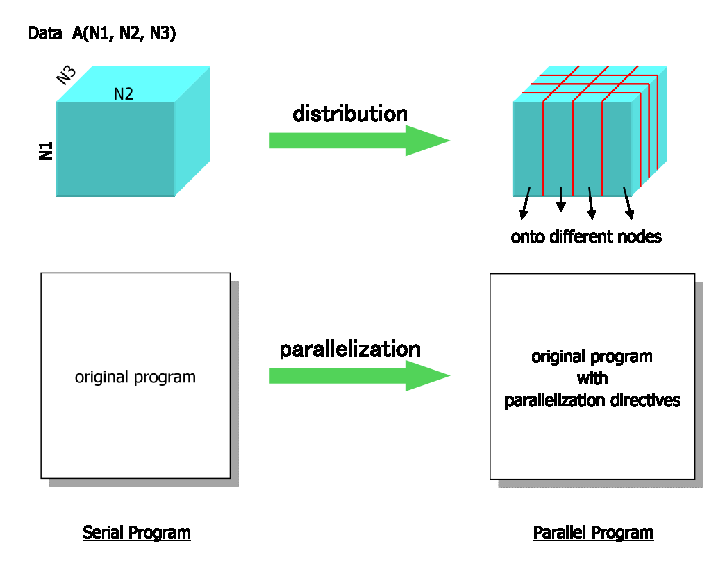
\includegraphics[width=12cm]{figs/Fig2.eps}
  \caption{Parallelization by the global-view programming model}
\label{fig2}
\end{myfigure}

\section{Local-view programming model}

The local-view programming model is suitable for 
programs that explicitly describe the algorithm of each node and for explicit
remote data reference (Figure \ref{fig3}). Since MPI is
considered to have a local view, the local-view programming model of \XMP has high
interoperability with MPI.

For the local-view programming model,
the language extension and some directives are provided. The coarray
notation taken from \CAF (CAF) is such an extension. For
example, in order to access an array element of {\tt A(i)} located on compute
node {\tt N},
the expression of {\tt A(i)[N]} is used. If the access is a value reference,
then communication to obtain the value occurs. If the access is to 
update the value, then communication to set a new value occurs.

\begin{myfigure}
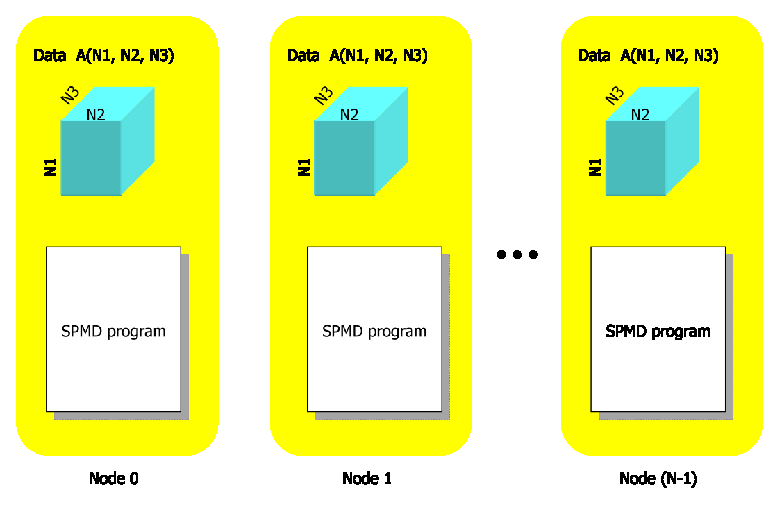
\includegraphics[width=12cm]{figs/Fig3.eps}
  \caption{Local-view programming model}
\label{fig3}
\end{myfigure}

\section{Interactions between global view and local view}

The node in
\XMP is used to distribute data or the computational
load. In the local view, the node is used in conjunction with the coarray
directive to reference data. In the application program, programmers
should choose an appropriate data model according to the structure of
the program. Figure \ref{fig4} illustrates the global view and the local view of data.

Data may have a global view and local view and can be
accessed from either view. \XMP provides some
directives to set the local name (alias) to the global data declared in
the global-view programming mode so that the data can also be referenced 
in the local-view programming model. It may be useful to optimize the
program by explicit remote data reference in the local-view programming model.


\begin{myfigure}
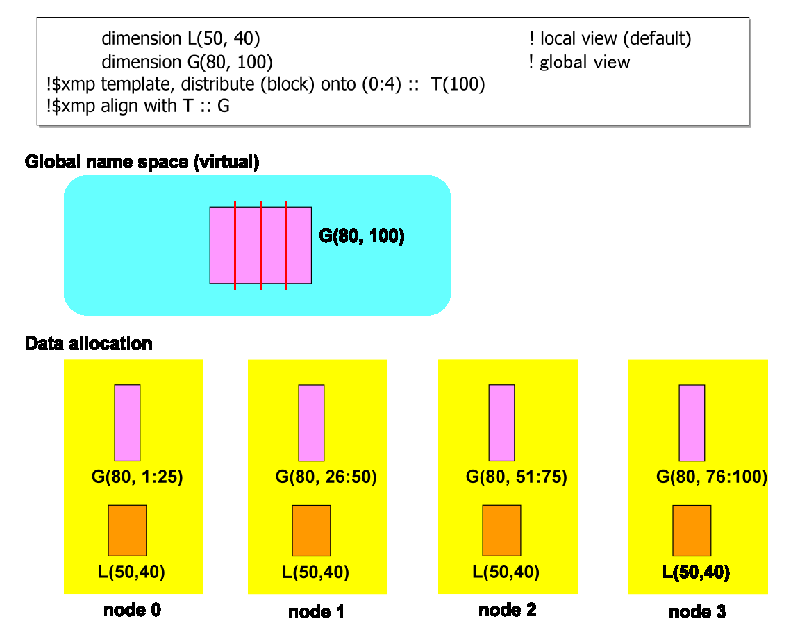
\includegraphics[width=12cm]{figs/Fig4.eps}
  \caption{Global view and local view}
\label{fig4}
\end{myfigure}

\section{Execution model and task}


In \XMP, a program begins as a single thread
of execution in each node. The set of nodes when starting a program is
referred to as the entire node set.

A task is a specific instance of executable
code and its data environment executed in a set of nodes. A task when
starting a program in the entire node set is called an initial task. The
initial task can generate a subtask, which is executed on a subset of the
nodes by the {\tt task} construct. A set of nodes executing the same task is
referred to as the set of executing nodes. If no {\tt task} construct is encountered, then a
program is executed as a single task, and its executing nodes are the entire node set.

If no directives are encountered, then a program is executed
locally. When the same codes are executed, almost the same computation is
performed in each node, which is referred to as duplicate execution. When the threads
encounter a {\tt loop} construct or an {\tt array} construct, the specified
loop is executed in parallel, so that each iteration is assigned to the
node where the specified data element is located. 

A new task is generated by
the {\tt task} construct. A code in the {\tt task} construct is executed
as a subtask executed in a specified node set. When a subroutine is
called in the context of the task, the subroutine is executed on its
executing nodes. 

For synchronization and communication between nodes, a set of
directives is provided. In the local-view programming model, coarray
features are adopted for remote data reference. Note 
that all synchronization and communication are specified explicitly by directives, and without such directives, no communications are
executed implicitly by the compiler.

\newcommand{\namelistlabel}[1]{\mbox{#1}\hfil}
\newenvironment{namelist}[1]{%
\begin{list}{}
       {\let\makelabel\namelistlabel
        \settowidth{\labelwidth}{#1}
        \setlength{\leftmargin}{1.3\labelwidth}
}
}{%
\end{list}}

\newcommand{\gitem}[1]{\item[{\parbox[b]{3.3cm}{\raggedleft \bf \Term{#1}}}]}


\section{Glossary}

\subsection{Language Terminology}

\begin{namelist}{entire node setxxxx}

\gitem{base language}

 A programming language that serves as the foundation of the {\XMP}
 specification.

\gitem{base program}

 A program written in a base language.

\gitem{structured block}

 For C, an executable statement, possibly compound, with a single entry
 at the top and a single exit at the bottom, or an OpenMP construct.
 For Fortran, a block of executable statements with a single entry at
 the top and a single exit at the bottom, or an OpenMP construct.

\gitem{procedure}

 A generic term used to refer to ``procedure'' (including subroutine and
 function) in Fortran and ``function'' in C.

\gitem{directive}

 In C, a {\tt \#pragma}, and in Fortran, a comment, that specifies
 {\XMP} program behavior.

\gitem{declarative directive}

 An {\XMP} directive that may only be placed in a declarative context. A
 declarative directive has no associated executable user code, but
 instead has one or more associated user declarations.

\gitem{executable directive}

 An {\XMP} directive that is not declarative; it may be placed in an
 executable context.

\gitem{construct}

 An {\XMP} executable directive (and for Fortran, the paired end
 directive, if any) and the associated statement, loop or structured
 block, if any.

%, not
%including the code in any called routines; i.e., the lexical extent of an
%executable directive.

\gitem{global construct}

 A construct that is executed collectively and synchronously by all
 nodes in the executing node set. Global constructs are further
 classified into two groups of {\it global communication constructs},
 such as {\tt gmove}, {\tt barrier}, etc., which specify communication
 or synchronization, and {\it work mapping constructs}, such as {\tt
 loop}, {\tt array} and {\tt tasks}, which specify parallelization of
 loops, array assignments or a set of tasks.

\gitem{template}

 A dummy array that represents an index space to be distributed onto a
 node set, which serves as the ``template'' of parallelization in
 {\XMP} and can be considered to abstract, for example, a set of grid
 points in the grid method or particles in the particle method.
%
 A template is used in an {\XMP} program to specify the data and the
 work mapping.

%A dummy array used to express an index space associated
%with an array. Template is also used to describe the iteration space of
%a loop. A template has a name, a dimension, and an upper and  lower
%bound for each dimension as attributes.

\gitem{data mapping}

 Allocating elements of an array to nodes in a node set by specifying
 with the {\tt align} directive that the array is aligned with a
 distributed template.

%\gitem{work}

\gitem{work mapping}

 Assigning iterations of a loop, elements of an array assignment, or
 tasks in a task set to nodes in a node set by specifying with one of
 the work mapping constructs that the loop, the assignment, or the set
 is aligned with a template or distributed onto a node array.

%\subsection*{\Term{data mapping}}
%The combination of the alignment and
%distribution attributes used to describe how a data object is
%allocated to nodes.
%
%\subsection*{\Term{work mapping}}
%Assignment of iterations to nodes in
%a parallel loop and tasks to nodes.

\gitem{global}

 A data or a work is {\it global} if and only if there is only one
 instance of it shared by all nodes in the executing node set.

\gitem{local}

 A data or a work is {\it local} if and only if there is a replicated
 instance of it in each node in the executing node set.

\gitem{global-view model}

 A model of programming or parallelization on which parallel programs
 are written by specifying how to map global data and works onto nodes.

\gitem{local-view model}

 A model of programming or parallelization on which parallel programs
 are written by specifying how each node owns local data and does local
 works.

%Execution of a program has side-effects only on the data in the node. In
%this case, no communication with other nodes occurs .

%\subsection*{\Term{non-local}}
%
%Execution of a program requires
%communication with other nodes and has side-effects with respect to other
%nodes. 

\end{namelist}


\subsection{Node Terminology}

\begin{namelist}{entire node setxxxx}

\gitem{phisical node}

 A computing component of a distributed-memory multicomputer, which has
 its own main memory and is connected with each other via an
 interconnect. A node may contain multiple cores sharing the main
 memory.

%In a distributed memory system, a computation node, which may have
%several cores sharing main memory, has its own local memory. Each node
%is connected through a network. An \XMP program begins as a single
%thread of execution in each node.

\gitem{(logical) node}

 An execution entity managed and assigned to a phisical node at runtime
 by the {\XMP} runtime system, which has its own memory and can
 communicate with other nodes. A node can execute one or more threads
 concurrently.

\gitem{node set}

 A set of nodes.

\gitem{entire node set}

 A node set that contains all of the nodes participating in the
 execution of an XcalbleMP program.

\gitem{(current) executing node set}

 A node set that contains all of the nodes participating in the
 execution of a procedure, a statement, a construct, etc. of an
 XcalableMP program is called its executing node set. The current
 executing node set can be modified by the {\tt task}, {\tt array}, or
 {\tt loop} direcitives. Note that the executing node set of the main
 routine is the entire node set.

\gitem{node array}

 An entity of the same form as a Fortran array that represents a node
 set in XcalableMP programs. Each element of a node array represents a
 node in the corresponding node set. A node array is declared by the
 {\tt nodes} directive.

\gitem{parent node set}

 The parent node set of a node set is the last executing node set, which
 encounterd the innermost {\tt task}, {\tt loop}, or {\tt array}
 construct that it is executing.

%\gitem{node number}
%
% A number assigned to a node, which is associated with a node array and
% determined according to Fortran's array element order (i.e. row-major).

%\subsection*{\Term{node number}}
%
%A unique number assigned to each of the nodes in the entire node
%set. The number starts from 1, larger than or equal to 1 and less than
%and equal to the number of nodes.Note that the mapping from the node
%number to the MPI rank is decided by the system. The image index of 
%the coarray mapping to the entire node set is equal to the node number. 
%
%\subsection*{\Term{entire node set}, \Term{entire set of nodes}}
%All nodes executing the program, or a set of these nodes. The entire node set is
%decided when staring the program.
%
%\subsection*{\Term{executing node set}, \Term{executing nodes}}
%A node set executing a certain region of a program. The executing node
%set that executes an entire program is the entire node set. The executing
%node set of a task is the node set that executes the task. 
%
%\subsection*{\Term{node array}}
%A multi-dimensional array containing nodes. The node array has a
%name and shape as it attributes.
%
%\subsection*{\Term{executing node array}}
%Node array that contains the executing node.

\end{namelist}


\subsection{Data Terminology}

\begin{namelist}{entire node setxxxx}

\gitem{global data}

 An array that is aligned with a template. Elements of a global data are
 distributed onto nodes according to the distribution of the
 template. As a result, each node owns a part of a global data (called
 {\it local section}), and can access directly it but cannot those on
 the other nodes.

%Data declared as a distributed array and shared by nodes.

\gitem{local data}

 Data that is not global. Each node owns a replica of a local data,
 and can access directly it but cannot those on the other nodes. Note
 that the replicas of a local data do not necessarily have the same
 value.

%Data is allocated in each node and is referenced only
%within the node.

\gitem{replicated data}

 A data whose storage is allocated on multiple nodes. A replicated data
 is either a local data or a global data replicated by an {\tt align}
 directive.

\gitem{distribution}

 Assigning each element of a template to nodes in a node set in a
 specified manner. In the broad sense, it means that of an array, a
 loop, etc.

% The partition of the index space of a data object among a set of nodes
% according to a given pattern. The {\tt distribute} directive is used to 
% map the elements of a template onto a set of nodes.

\gitem{alignment}

 Associating each elemtent of an array, a loop, etc. with an element of
 the specified template. An Element of an array, a loop, etc. is
 necessarily mapped to the same node as its associated element of the
 template is.

% An attribute of a data object that establishes the relationship between
% data objects for distribution. The {\tt align} directive is used to
% describe the correspondence of the element of the data and the
% template.

\gitem{local section}

 A section of a global data that is allocated as an array on each node
 at runtime.
%
 The local section of a global data includes its shadow objects.

\gitem{shadow}

 An additional area of the local section of a distributed array, which
 is used to keep the elements that have to be moved in from neighboring
 nodes.

% A data area used to keep neighbor elements temporarily in a
% distributed array.
% Shadow is an attribute of a distributed array that
% is declared by the {\tt shadow} directive and is updated by the {\tt
% reflect} directive.

\end{namelist}


\subsection{Work Terminology}

\begin{namelist}{entire node setxxxx}

\gitem{task}

 A specific instance of executable codes that is defined by the {\tt
 task} construct and executed by a node set specified by its {\tt on}
 clause.

%A specific instance of executable code and
%its data environments executed in a set of nodes. In the context of
%the program text, a set of statement executed by a set of nodes. A task
%can be nested, and a nested task is executed as a subtask of an outer task.

%\subsection*{\Term{replicated execution}}
%
%Execution of the same code in different nodes. If the state at the
%starting point is the same and the execution has only local
%side-effects, then the local state in each node remains the same.

%\gitem{collective}
%
%      A construct is {\it collective} if and only if it must be executed 
%      synchronously and with the exact same directive and associated
%      statements by every nodes in the executing node set. The behavior
%      of an {\XMP} program is not specified if a collective construct is
%      not executed {\it collectively}.

%An operation must be executed by every
%node in the executing node set in order to perform an operation together.

\end{namelist}


\subsection{Communication and Synchronization Terminology}

To be added.

\subsection{Local-view Terminology}

\begin{namelist}{entire node setxxxx}

\gitem{local alias}

 An alias to the local section of a global data, that is, a distributed
 array. A local alias can be used in {\XMP} programs in the same way as
 normal local data can.

\gitem{coarray}

 A special local data that can be accessed directly by other nodes with
 a specific notation (i.e. the {\it image index} corresponding to the
 target node in the square brackets) added to the end of the array
 reference syntax.
%
 Every coarray is associated explicitly or implicitly with a node
 set and allocated on each node of the node set.

 The coarray feature of {\XMP} is based on that of the upcoming Fortran
 2008 standard.

%\gitem{image}

\gitem{image index}

 A special identifier, in the style of an integer sequence, which is
 used in a coarray reference to specify a target node. An image index in
 the square brackets of a coarray reference refers to a corresponding
 node in the node set with which the coarray is associated. The
 correspondence is determined according to Fortran's array element order
 (i.e. row-major).

%A number assigned to
%each image of the coarray. The value is equal to or greater than 1. 
%Note that the image index of the coarray mapping to the entire node set is
%identical to the node number.

\end{namelist}

\cleardoublepage

\chapter{Directives}\index{directive}

This chapter describes the syntax and behavior of {\XMP} directives.
In this document, the following notation is used to describe {\XMP}
directives. 

\vspace{0.5cm}%

\begin{tabular}{ll}
{\tt xxx} & {\tt type-face} characters are used to indicate literal type characters. \\
{\it xxx...} & If the line is followed by ``...'', then xxx can be
repeated. \\
{\it [xxx]} & {\it xxx} is optional. \\
\verb![F]! & The following lines are effective only in {\XMPF}. \\
\verb![C]! & The following lines are effective only in {\XMPC}. \\
\end{tabular}

\section{Directive Format}

\subsection{General Rule}

In {\XMPF}, {\XMP} directives are specified using special comments that
are identified by unique sentinels {\tt\verb|!$xmp|}. An {\XMP}
directive follows the rules for comment lines of either the Fortran free
or fixed source form, depending on the source form of the surrounding
program unit\footnote{Consequently, the rules of comment lines that an
{\XMP} directive follows is the same as the ones that an {\OMP}
directive follows.}. {\XMPF} directives are case-insensitive.

\vspace{0.5cm}

\Syntax{directive}
\begin{tabular}{ll}
\verb![F]! & \verb|!$xmp| {\it directive-name clause} \\
\end{tabular}

\vspace{0.5cm}

In {\XMPC}, {\XMP} directives are specified using the \verb|#pragma|
mechanism provided by the {\C} standards. {\XMPC} directives are
case-sensitive.

\vspace{0.5cm}

Syntax{directive}
\begin{tabular}{ll}
\verb![C]! & \verb|#pragma xmp| {\it directive-name clause} \\
\end{tabular}

\vspace{0.5cm}

%Additionally, in {\Fort}, directives of the {\it attribute form}
%analogous to type declaration statements in Fortran using the ``{\tt
%::}'' punctuation can also be used.

Directives are classified as declarative directives and executable
directives. The declarative directive is a directive that may only be
placed in a declarative context. A declarative directive has no
associated executable user code. The scope rule of declarative
directives obeys that of the declaration statements in the base
language.
%
For example, in {\XMPC}, a node array declared by a {\tt nodes}
directive is visible in the range from the declaring point to the end of
the function when placed within a function, or of the file when
placed outside any functions,
%
and, in {\XMPF}, a node array declared by a {\tt nodes} directive is
visible within either the program unit, the derived-type declaration
or the interface body that immediately encloses the directives.

The executable directives are placed in an executable context. A
stand-alone directive is an executable directive that has no associated
user code, such as a {\tt barrier} directive.
%
An executable directive and its associated user code make up an
{\XMP} construct, as in the following format:

\vspace{0.5cm}

\begin{tabular}{ll}
\verb![F]! & \verb|!$xmp| {\it directive-name clause} ...\\
 & \hspace{0.5cm} {\it structured-block} \\
\end{tabular}

\vspace{0.3cm}

\begin{tabular}{ll}
\verb![C]! & \verb|#pragma xmp| {\it directive-name clause} ...\\
 & \hspace{0.5cm} {\it structured-block} \\
\end{tabular}

\vspace{0.5cm}

Note that, in {\XMPF}, a corresponding {\tt end} directive is required
for some executable directives such as {\tt task} and {\tt tasks} and,
in {\XMPC}, the associated statement can be a compound-statement.

%\vspace{0.5cm}
%
%\begin{tabular}{ll}
%\verb![F]! & \verb|!$xmp tasks| \\
% & \hspace{0.5cm} {\it structured-block} \\
% & \hspace{0.5cm} ... \\
% & \verb|!$xmp| {\tt end tasks}\\
%\end{tabular}


\subsection{Combined Directive}

\subsubsection*{Synopsis}

For {\XMP} {\Fort}, multiple attributes can be specified
in one combined declarative directive, which is analogous to type
declaration statements in Fortran using the ``{\tt ::}'' punctuation.

\subsubsection*{Syntax}

\begin{center}
\begin{tabular}{llll}
\verb![F]! & \verb|!$xmp| {\it combined-directive} & {\bf is} & {\it
 combined-attribute} {\openb}, {\it combined-attribute}
 {\closeb}... {\tt ::} \\
 & & & {\it combined-decl} {\openb}, {\it combined-decl}
 {\closeb}...
\end{tabular}
\end{center}

{\it combined-attribute} is one of:

\vspace{0.3cm}

\begin{tabular}{ll}
 \hspace{0.5cm} & {\tt nodes} \\
 & {\tt template} \\
 & {\tt distribute} \verb|(|{\it dist-format} {\openb}, {\it
     dist-format}{\closeb}... \verb|)| {\tt onto} {\it nodes-name} \\
 & {\tt align} \verb|(| {\it align-source} {\openb}, {\it
     align-source}{\closeb}... \verb|)| \\
 & \hspace{4cm}{\tt with} {\it template-name} \verb|(|{\it
     align-subscript} {\openb}, {\it
     align-subscript}{\closeb}... \verb|)| \\
 & {\tt shadow} \verb|(| {\it shadow-width} {\openb},
     {\it shadow-width}{\closeb}... \verb|)| \\
 & {\tt dimension} \verb|(| {\it explicit-shape-spec} {\openb},
     {\it explicit-shape-spec}{\closeb}... \verb|)|
\end{tabular}

\vspace{0.3cm}

and {\it combined-decl} is one of:

\vspace{0.3cm}

\begin{tabular}{ll}
 \hspace{0.5cm} & {\it nodes-decl} \\
 & {\it template-decl} \\
 & {\it array-name}
\end{tabular}

\subsubsection*{Description}

A combined directive is interpreted as if an object corresponding to
each {\it combined-decl} is declared in a directive corresponding to
each {\it combined-attribute}, where all restrictions of each directive,
in addition to the following ones, are applied.

\subsubsection*{Restrictions}

\begin{itemize}
 \item The same kind of {\it combined-attribute} must not appear more
       than once in a given {\it combined-directive}.
 \item If the {\tt dimension} attribute appears in a {\it
       combined-directive}, any object to which it applies must be
       declared with either the {\tt template} or the {\tt nodes}
       attribute.
\end{itemize}

\section{\Directive{nodes} Directive}

\subsubsection*{Synopsis}

%The {\tt nodes} directive declares a node array with a name, a shape,
%and some attributes.

The {\tt nodes} directive declares a named node array.

\Syntax{nodes}
\subsubsection*{Syntax}

{\small
\begin{tabular}{ll}
\verb![F]!&\verb|!$xmp| {\tt nodes} {\it nodes-name} \verb|(|
     {\it nodes-spec} {\openb}, {\it nodes-spec}
     {\closeb}... \verb|)| \\
\verb![F]!&\verb|!$xmp| {\tt nodes} {\it nodes-name} \verb|(|
     {\it nodes-spec} {\openb}, {\it nodes-spec}
     {\closeb}... \verb|)| {\tt = *}\\
\verb![F]!&\verb|!$xmp| {\tt nodes} {\it nodes-name} \verb|(|
     {\it nodes-spec} {\openb}, {\it nodes-spec}
     {\closeb}... \verb|)| {\tt =} {\it nodes-ref}\\
& \\
\verb![C]!&\verb|#pragma xmp| {\tt nodes} {\it nodes-name}
     \verb|(| {\it nodes-spec} {\openb}, {\it nodes-spec}
     {\closeb}... \verb|)| \\
\verb![C]!&\verb|#pragma xmp| {\tt nodes} {\it nodes-name}
     \verb|(| {\it nodes-spec} {\openb}, {\it nodes-spec}
     {\closeb}... \verb|)| {\tt = *} \\
\verb![C]!&\verb|#pragma xmp| {\tt nodes} {\it nodes-name}
     \verb|(| {\it nodes-spec} {\openb}, {\it nodes-spec}
     {\closeb}... \verb|)| {\tt =} {\it nodes-ref} \\
\end{tabular}
}

\vspace{0.3cm}

where {\it nodes-spec} must be one of:

\hspace{\hsize}

\begin{tabular}{ll}
 \hspace{0.5cm} & {\it int-expr} \\
 \hspace{0.5cm} & {\tt *} \\
\end{tabular}

%{\small
%\begin{tabular}{ll}
%\verb![F]!&\verb|!$xmp| {\tt nodes} {\it nodes-name}({\it nodes-size})
% [, {\it nodes-name}({\it nodes-size})]... \\
%\verb![F]!&\verb|!$xmp| {\tt nodes} {\it nodes-name}({\it nodes-size})
%     [, {\it nodes-name}({\it nodes-size})]... {\tt = *}\\
%\verb![F]!&\verb|!$xmp| {\tt nodes} {\it nodes-name}({\it nodes-size})
%     [, {\it nodes-name}({\it nodes-size})]... {\tt =} {\it nodes-ref}\\
%& \\
%\verb![C]!&\verb|#pragma xmp| {\tt nodes} {\it nodes-name}({\it
%     nodes-size}) [, {\it nodes-name}({\it nodes-size})]... \\
%\verb![C]!&\verb|#pragma xmp| {\tt nodes} {\it nodes-name}({\it
%     nodes-size}) [, {\it nodes-name}({\it nodes-size})]... {\tt = *} \\
%\verb![C]!&\verb|#pragma xmp| {\tt nodes} {\it nodes-name}({\it
%     nodes-size}) [, {\it nodes-name}({\it nodes-size})]... {\tt =} {\it
%     nodes-ref}\\
%\end{tabular}
%}
%\vspace{0.3cm}

%where {\it nodes-size} is a positive integer expression.

\subsubsection*{Description}

The {\tt nodes} directive declares a node array that corresponds to a
node set.

The first form is used to declare a node array that corresponds to the
entire node set.
%The second and third forms declare a new node array with a name, a
%dimension, and a size in order to reference a set of nodes.
The second form is used to declare a node array that corresponds to the
executing node set.
%The ``{\tt *}'' symbol specifies the current executing node set.
The third form is used to declare a node array that corresponds to the
node set specified by {\it nodes-ref}.

%If {\it map-type} is specified as {\tt regular}, then the order of nodes in
%the node array follows that of the {\Fort} array. Therefore, in the first
%form, the node number is used to order nodes in the node array with
%{\Fort} array ordering. In the second and third forms, the nodes are
%ordered according to the sequence association with referenced nodes.  
%
%If no {\it map-type} is specified, then the ordering nodes in the node array are
%system dependent. It is desirable to order the nodes in order to make use of
%the network topology for efficient communication. 

If {\it node-size} in the last dimension is ``{\tt *}'', then the size
of the node array is automatically adjusted according to the total size
of the entire node set in the first form, the executing node set in the
second form, or the referenced node set in the third form.

\subsubsection*{Restrictions}

\begin{itemize}
%\item {\it nodes-name} is an identifier in class (1) and must not
%  conflict with other names in class (1).
\item {\it nodes-name} must not conflict with any other local name in
      the same scoping unit.
\item In {\Fort}, the second form cannot be used in either the main
      program or a module.
\item {\it nodes-spec} can be ``{\tt *}'' only in the last dimension.
\item {\it nodes-ref} must not reference {\it nodes-name} either
      directly or indirectly.
\item If no {\it nodes-spec} is ``{\tt *}'', then the product
      of all {\it nodes-spec} must be equal to the total size of the
      entire node set in the first form, the executing node set in the
      second form, or the referenced node set in the third form.
%
%      The referenced node set must consist of all nodes in the first form,
%      the executing node set in the second form, and the node set
%      referenced by {\it nodes-ref} in the third form. 
\item {\it nodes-subscript} in {\it nodes-ref} must not be ``{\tt *}''.
\end{itemize}

\subsubsection*{Examples}
\Example{nodes}

The following are examples of the first and the third forms appeared in
the main program. Since the node array {\tt p}, which corresponds to the
entire node set, is declared to be of size 16, this program must be
executed on 16 nodes.

%Since the declaration of node array {\tt p} specifies
%16 nodes as its size, this program must be executed with 16 nodes.

%Since {\tt regular} is not specified, it is not guaranteed that {\tt
%Ar(1)} and {\tt p(3)} are the same node, and the node number of {\tt
%z(1,1)} is 1.

\vspace{0.5cm}

\begin{minipage}{0.45\hsize}
\begin{center}
\begin{Fexample}
      program main
!$xmp nodes p(16)
!$xmp nodes q(4,*)
!$xmp nodes r(8)=p(3:10)
!$xmp nodes z(2,3)=(1:6)
      ...       
      end program 
\end{Fexample}
\end{center}
\end{minipage}
%
\begin{minipage}{0.45\hsize}
\begin{center}
\begin{CexampleR}
int main() {
#pragma xmp nodes p(16)
#pragma xmp nodes q(4,*)
#pragma xmp nodes r(8)=p(3:10)
#pragma xmp nodes z(2,3)=(1:6)
    ...
}
\end{CexampleR}
\end{center}
\end{minipage}

\vspace{0.5cm}

%Example using the regular option. Since node array {\tt p} is declared
%without the regular option, it is not guaranteed that {\tt p(1), p(2)}
%have the node number 1, 2, ... and so on. The node array {\tt q} with the 
%regular option has the order in which
%{\tt q(1,1), q(2,1), q(3,1), q(4,1), q(1,2), ...} have node numbers
%1,2,3,4,5, ... In node array z with the regular option,
%{\tt z(1,1), z(2,1), z(1,2), z(2,2), z(1,3), z(2,3), ...} have the
%node numbers 1, 2, 3, 4, 5, 6, ...
%
%\begin{Fexample}
%      program main
%!$xmp nodes p(16)
%!$xmp nodes(regular) q(4,*)
%!$xmp nodes(regular) r(8)=p(3:10)
%!$xmp nodes(regular) z(2,3)=(1:6)
%      ...
%      end program
%\end{Fexample}

The following is an example of a node declaration in a procedure.
Since {\tt p} is declared in the second form to be of size 16 and
correspond to the executing node set, the invocation of the {\tt foo}
function must be executed by 16 nodes.
%
The node array {\tt q} is declared in the first form and corresponds to
the entire node set. The node array {\tt r} is declared as a subset of
{\tt p}, and {\tt x} as a subset of {\tt q}.

%The declaration for the node array {\tt q} of the first form
%declares the node array for the entire node set. The node array {\tt r}
%is a subset of {\tt p}, and the node array of {\tt x} is a subset of
%{\tt q}.

\begin{Fexample}
      function foo()
!$xmp nodes p(16)=*
!$xmp nodes q(4,*)
!$xmp nodes r(8)=p(3:10)
!$xmp nodes x(2,3)=q(1:2,1:3)
      ...
      end function
\end{Fexample}


\subsection{Node Reference}

\subsubsection*{Synopsis}

The \Term{node reference} expression is used to reference a subset of a
node set.

\subsubsection*{Syntax}
\Syntax{node reference}

A node reference {\it nodes-ref} is specified by either node number
or the name of a node array.

\begin{center}
\begin{tabular}{lll}
{\it nodes-ref} & {\bf is} & \verb|(| {\it nodes-subscript} \verb|)|\\ 
                & {\bf or} & {\it nodes-name} {\openb}\verb|(| {\it nodes-subscript}
	 {\openb}, {\it nodes-subscript} {\closeb}... \verb|)|{\closeb} \\
\end{tabular}
\end{center}
%
\vspace{0.3cm}
%
where {\it nodes-subscript} must be one of:

\hspace{\hsize}

\begin{tabular}{ll}
 \hspace{0.5cm} & {\it int-expr} \\
 \hspace{0.5cm} & {\it triplet} \\
 \hspace{0.5cm} & {\tt *} \\
\end{tabular}

%\begin{center}
%\begin{tabular}{ll}
%{\it nodes-ref} & {\it node-number-ref} $\vert$ {\it named-nodes-ref} \\
%{\it node-number-ref} & {\it node-number} $\vert$ ([{\it
%     node-number}]:[{\it node-number}][:{\it int-expr}]) \\
%& {\it node-number} is a positive number. \\
%{\it named-nodes-ref} & {\it nodes-name} [ ( {\it nodes-subscript}
%[,  ...] ) ] \\
%{\it nodes-subscript} & {\it int-expr} $\vert$ {\it triplet} $\vert$ {\tt *} \\
%\end{tabular}
%\end{center}

\subsubsection*{Description}

Node reference by node number represents one node specified by the node 
number, or a node set specified by a triplet that represents a set of
node numbers.

Node reference by name represents a node set specified by the name of a
node array or its subarray.

%The subscript of the subarray of a node array must be either an integer,
%a triplet, or ``{\tt *}''. The notation of the subarray using a triplet
%in the subscript is the same as that in {\Fort}. 

Specifically, the ``{\tt *}'' symbol apperared as {\it nodes-subscript}
in a dimension of {\it nodes-ref} is interpreted by each node at runtime
as its position (coordinate) in the dimension of the referenced node
array.
%The ``{\tt *}'' symbol in {\it nodes-subscript} in a subarray of a
%node array specifies a subscript associated with the executing node in
%the node array of the executing node set.
%
Thus, a node reference {\tt p($s_1$, ..., $s_{k-1}$, *, $s_{k+1}$, ...,
$s_n$)} is interpreted as {\tt p($s_1$, ..., $s_{k-1}$, $j_k$,
$s_{k+1}$, ..., $s_n$)} on the node corresponding to {\tt p($j_1$, ...,
$j_{k-1}$, $j_k$, $j_{k+1}$, ..., $j_n$)}.

%Thus, the following node is referenced by name with the $k$-th subscript
%``{\tt *}'':
%
%\begin{center}
%{\tt p($s_1$, ..., $s_{k-1}$, *, $s_{k+1}$, ..., $s_n$)} 
%\end{center}
%where, with the exception of $s_k$, subscripts $s_i$ must not be ``{\tt *}'', 
%is evaluated at the node 
%\begin{center}
%{\tt p($j_1$, ..., $j_{k-1}$, $j_k$, $j_{k+1}$, ..., $j_n$)} 
%\end{center}
%where $j_i$ is an integer, in
%\begin{center}
%{\tt p($s_1$, ..., $s_{k-1}$, $j_k$, $s_{k+1}$, ..., $s_n$)}.
%\end{center}

Note that ``{\tt *}'' can be used only as the node reference in
the {\tt on} clause of some executable directives.

%This node reference composes the node set using nodes with the $k$-th
%subscript $j_k$. The same rule is applied even if more than two
%subscripts are ``{\tt *}''. This notation can be used only in the node
%reference of the on clause in executable directives. 

\subsubsection*{Examples}

Assume that {\tt p} is the name of a node array and that {\tt m} is an
integer variable.

\begin{itemize}
\item As a target node array in the {\tt distribute} directive

\Example{distribute}
\begin{tabular}{l}
\verb|!$xmp distribute a(block) onto p| \\
\end{tabular}%$

\item To specify a node set to which the declared node array corresponds
      in the second form of the {\tt nodes} directive

\Example{nodes}
\begin{tabular}{l}
\verb|!$xmp nodes r(2,2,4) = p(1:4,1:4)| \\
\verb|!$xmp nodes r(2,2,4) = (1:16)| \\
\end{tabular}

\item To specify a node array that corresponds to the executing node set
      of a task in the {\tt task} directive

\Example{task}
\begin{tabular}{l}
\verb|!$xmp task on p(1:4,1:4)| \\
\verb|!$xmp task on (1:16)| \\
\verb|!$xmp task on p(:,*)| \\
\verb|!$xmp task on (m)| \\
\end{tabular}

\item To specify a node array with which the iterations of the loop are
      aligned in the {\tt loop} directive

%In the {\tt loop} directive, sets of executing nodes are specified
%      for the iterations.

\Example{loop}
\begin{tabular}{l}
\verb|!$xmp loop (i) on p(lb(i):lb(i+1)-1)| \\
\end{tabular}%$

\item To specify a node array that corresponds to the executing node set
      in the {\tt barrier} and the {\tt reduction} directive

%In {\tt barrier} directive and the {\tt reduction} directive,
%executing nodes are specified. 

\Example{barrier}
\Example{reduction}
\begin{tabular}{l}
\verb|!$xmp barrier on p(5:8)| \\
\verb|!$xmp reduction (+:a) on p(*,:)| \\
\end{tabular}

\item To specify the source node and the node array that corresponds to
      the executing node set in the {\tt bcast} directive 

%In the {\tt bcast} directive, a source node and executing nodes are specified.

\Example{bcast}
\begin{tabular}{l}
\verb|!$xmp bcast b from p(k) on p(:)| \\
\end{tabular}
\end{itemize}

%\subsubsection*{Examples}
%\Example{nodes}
%\Example{tasks}
%\Example{task}
%\Example{end task}
%\Example{end tasks}
%
%\begin{minipage}{0.45\hsize}
%\begin{center}
%\begin{Fexample}
%      subroutine caller
%!$xmp nodes p(1000)
%      real a(100,100)
%      ...
%!$xmp tasks
%!$xmp  task on p(1:500)
%        call task1(a)
%!$xmp  end task
%!$xmp  task on p(501:800)
%        call task1(a)
%!$xmp  end task
%!$xmp  task on p(801:1000)
%        call task1(a)
%!$xmp  end task
%!$xmp end tasks
%      ...
%      end do
%\end{Fexample}
%\end{center}
%\end{minipage}
%\begin{minipage}{0.45\hsize}
%\begin{center}
%\begin{FexampleR}
%      subroutine task1(a)
%      ...
%!$xmp nodes q(*)
%      real a(100,100)
%      ...
%      end subroutine
%\end{FexampleR}
%\end{center}
%\end{minipage}
%\vspace{1cm}


\subsection{Correspondence between Node Arrays}

To be described.

\subsection{Executing Node Sets}

To be described.

\section{Template and Data Mapping Directives}

\subsection{{\tt template} Directive}

\subsubsection*{Synopsis}

The {\tt \Directive{template}} directive declares a template. 

\subsubsection*{Syntax}
\Syntax{template}

\begin{tabular}{ll}
\verb![F]! & \verb|!$xmp| {\it template-name} ( {\it template-spec} 
[, {\it template-spec} ] ... ) \\
& \\
\verb![C]! & \verb|#pragma xmp|  {\it template-name} ( {\it template-spec} 
[, {\it template-spec} ] ... ) \\
\end{tabular}
\vspace{0.3cm}

where {\it template-spec} must be one of:

\hspace{\hsize}

\begin{tabular}{ll}
 \hspace{0.5cm} & [{\it int-expr} {\tt :}] {\it int-expr} \\
 \hspace{0.5cm} & {\tt :} \\
\end{tabular}

\subsubsection*{Description}

The {\tt template} directive declares a template with the shape specified by
the sequence of {\it template-spec}. If every {\it template-spec} is
``:'', then the shape of the template is initially undefined. This
template must not be referenced until the shape is defined by {\it
template\_fix} directives (see section \ref{subsec:template_fix
directive}) at runtime. If {\it int-expr} is specified as {\it
template-spec}, then the default lower bound is 1.

\subsubsection*{Restrictions}

\begin{itemize}
\item Every {\it template-spec} must be either [{\it int-expr} {\tt :}] {\it
  int-expr} or ``:''.
\end{itemize}

\subsection{Template Reference}

\subsubsection*{Synopsis}

The \Term{template reference} expression is used to reference a subset of
the referenced template.

\subsubsection*{Syntax}
\Syntax{template reference}

\begin{center}
\begin{tabular}{ll}
{\it template-ref} & {\it template-name} [ ( {\it template-subscript}
[,  ...] ) ] \\
{\it template-subscript} & {\it int-expr} $\vert$ {\it triplet} $\vert$
     {\tt *} \\
\end{tabular}
\end{center}

\subsubsection*{Description}

The template reference refers to a subarray of the template array.  

The subscript
of the subarray of a template array must be either an integer, a
triplet, or ``{\tt *}''. The notation of the subarray using a triplet in
the subscript is the same as that in \Fort. 

\subsubsection*{Examples}

Assume that {\tt t} is a template name. 

\begin{itemize}
\item In the {\tt task} directive, a set of executing nodes is indirectly specified for the task.

\Example{task}
\begin{tabular}{l}
\verb|!$xmp task on t(1:m,1:n)| \\
\verb|!$xmp task on t| \\
\end{tabular}

\item In the {\tt loop} directive, an element of the template at which each loop iteration is aligned.

\Example{loop}
\begin{tabular}{l}
\verb|!$xmp loop (i) on t(i-1)| \\
\end{tabular}

\item In the {\tt array} directive, a template which the following array assignment statement is aligned with.

\Example{array}
\begin{tabular}{l}
\verb|!$xmp array on t(1:n)| \\
\end{tabular}

\item In the {\tt barrier}, {\tt reduction}, and {\tt bcast} directives,
executing nodes are specified indirectly. 

\Example{barrier}
\Example{reduction}
\begin{tabular}{l}
\verb|!$xmp barrier on t(1:n)| \\
\verb|!$xmp reduction (+:a) on t(*,:)| \\
\verb|!$xmp bcast b from p(k) on t(1:n)| \\
\end{tabular}

\end{itemize}

\subsection{{\tt distribute} Directive}

\subsubsection*{Synopsis}

The {\tt \Directive{distribute}} directive specifies a distribution of
templates.

\subsubsection*{Syntax}
\Syntax{distribute}

\begin{tabular}{ll}
\verb![F]! & \verb|!$xmp| {\tt distribute} {\it template-name} 
({\it dist-format} [, {\it dist-format}]... ) {\tt onto} {\it nodes-name} \\
& \\
\verb![C]! & \verb|#pragma xmp| {\tt distribute} {\it template-name} 
({\it dist-format} [, {\it dist-format}]... ) \\
& \hspace{3cm}{\tt onto} {\it nodes-name} \\
\end{tabular}
\vspace{0.3cm}

where {\it dist-format} must be one of:

\begin{tabular}{ll}
 \hspace{0.5cm} & {\tt *} \\
 & {\tt block} \\
 & {\tt cyclic} [ ( {\it int-expr} ) ] \\
 & {\tt gblock} ( {\tt *} $\vert$ {\it int-array} ) \\
\end{tabular}

\subsubsection*{Description}

According to the specified distribution format, a template is distributed
onto a node set. The dimension of the node set appearing in an {\tt
onto} clause corresponds, in left-to-right order, with the dimension of
the distributed template for which the corresponding {\it dist-format} is
not ``{\tt *}''. 

The interpretation of {\it dist-format} is as follows:

\begin{description}
\item[``{\tt *}'']
	   The corresponding dimension is not distributed.

\item[{\tt block}]
	   The corresponding dimension of the template is divided into
	   contiguous blocks of the same size, which are distributed onto
	   the corresponding dimension of the node set. Let {\tt d} be
	   the size of the corresponding dimension of the template, and
	   let {\tt p} be the size of the corresponding dimension of the
	   node sets. If {\tt d mod p} is not zero, then the dimension
	   of the template is divided into {\tt d/ceil(d/p)} blocks of
	   size {\tt ceil(d/p)} and one block of size {\tt d\%ceil(d/p)},
	   and each block is assigned sequentially to an index along the
	   corresponding dimension of the node set. Note that if {\tt
	   k = p-d/ceil(d/p)-1 > 0}, then there is no block for the last
	   {\tt k} indices.

\item[{\tt cyclic}]
	   Equivalent to {\tt cyclic(1)}.

\item[{\tt cyclic(n)}]
	   The corresponding dimension of the template is divided into
	   contiguous blocks of size {\tt n}, and these blocks are
	   distributed onto the corresponding dimension of the node set
	   in a round-robin manner.

\item[{\tt gblock(m)}]
	   {\tt m} is referred to as a mapping array. The corresponding
	   dimension of the template is divided into contiguous
	   blocks so that the i'th block is of size {\tt m(i)}, and
	   these blocks are distributed onto the corresponding dimension
	   of the node set.
\end{description}

If more than one {\tt gblock(*)} is specified in {\it dist-format},
then the template must not be referenced until the shape of the template
is defined by {\it template\_fix} directives at runtime.


\subsubsection*{Restrictions}

\begin{itemize}
\item The number of {\it dist-format} that is not ``{\tt *}'' must be
      equal to the rank of the node set specified by {\it nodes-name}.  
\item The array {\it int-array} in parentheses following {\tt gblock}
      must be an integer one-dimensional array, and its size must be
      equal to the size of the corresponding dimension of the node set
      specified by {\it nodes-name}.
\item Every element of the array {\it int-array} in parentheses
      following {\tt gblock} must be a non-negative integer.
\item The sum of the elements of the array {\it int-array} in 
      parentheses following {\tt gblock} must be equal to or greater
      than the size of the corresponding dimension of the template
      specified by {\it template-name}.
\end{itemize}

\subsubsection*{Examples}
\Example{nodes}
\Example{template}
\Example{distribute}

\begin{description}
\item[Example 1]
\hspace{\hsize}
\begin{Fexample}
      program main
!$xmp nodes p(8,5)
!$xmp template t(64,64,64)
!$xmp distribute t(*,cyclic,block) onto p
\end{Fexample}

The template {\tt t} is distributed in block format, as shown in the
following table.

\begin{center}
\begin{tabular}{|c|c|}
\hline
{\tt p(1)} & {\tt t(1:16)} \\
\hline
{\tt p(2)} & {\tt t(17:32)} \\
\hline
{\tt p(3)} & {\tt t(33:48)} \\
\hline
{\tt p(4)} & {\tt t(49:64)} \\
\hline
\end{tabular}
\end{center}

\item[Example 2]
\hspace{\hsize}
\begin{Fexample}
      program main
!$xmp nodes p(4)
!$xmp template t(64)
!$xmp distribute t(cyclic(8)) onto p
\end{Fexample}

The template {\tt t} is distributed in cyclic format of size eight, as
shown in the following table.

\begin{center}
\begin{tabular}{|c|c|}
\hline
{\tt p(1)} & {\tt t(1:8) t(33:40)} \\
\hline
{\tt p(2)} & {\tt t(9,16) t(41:48)} \\
\hline
{\tt p(3)} & {\tt t(17,24) t(49:56)} \\
\hline
{\tt p(4)} & {\tt t(25,32) t(57:64)} \\
\hline
\end{tabular}
\end{center}

\item[Example 3]
\hspace{\hsize}
\begin{Fexample}
      program main
!$xmp nodes p(8,5)
!$xmp template t(64,64,64)
!$xmp distribute t(*,cyclic,block) onto p
\end{Fexample}

The first dimension of the template {\tt t} is not distributed. The
second dimension is distributed onto the first dimension of the node set
{\tt p} in cyclic format. The third dimension is distributed onto the
second dimension of the node set {\tt p} in block format. The results
are as follows:

\begin{center}
\begin{tabular}{|c|c|}
\hline
{\tt p(1)} & {\tt t(1:64, 1:57:8, 1:13)} \\
\hline
{\tt p(2)} & {\tt t(1:64, 2:58:8, 1:13)} \\
\hline
... & ... \\
\hline
{\tt p(4)} & {\tt t(1:64), 8:64:8, 53:64)} \\
\hline
\end{tabular}
\end{center}

Note that the size of the third dimension is 64 and is not divisible by
the size of the second dimension of {\tt p}. Then, the sizes of a number
of blocks in the third dimension are different.

\end{description}

\subsection{{\tt align} Directive}

\subsubsection*{Synopsis}
The {\tt \Directive{align}} directive specifies that arrays are to be
mapped in the same way as a certain template.

\subsubsection*{Syntax}
\Syntax{align}

\begin{tabular}{ll}
\verb![F]! & \verb|!$xmp| {\tt align} {\it array-name}
( {\it align-source} [, {\it align-source}] ... ) \\
 & \hspace{3cm}{\tt with} {\it template-name}
({\it align-subscript} [, {\it align-subscript}] ... ) \\
 & \\
\verb![C]! & \verb|#pragma xmp| {\tt align} {\it array-name} 
{\tt [}{\it align-source}{\tt ]} [{\tt [}{\it align-source}{\tt ]}] ... \\
 & \hspace{3cm}{\tt with} {\it template-name}
({\it align-subscript} [, {\it align-subscript}] ... ) \\
\end{tabular}
\vspace{0.3cm}

where {\it align-source} must be one of:

\begin{tabular}{ll}
 \hspace{0.5cm} & {\tt scalar-int-variable} \\
 & {\tt *} \\
 & {\tt :} \\
\end{tabular}
\vspace{0.3cm}

and {\it align-subscript} must be one of:

\begin{tabular}{ll}
 \hspace{0.5cm} & {\tt scalar-int-variable} [ ( {\tt +} $\vert$ {\tt -} )
 {\it int-expr} ] \\
 & {\tt *} \\
 & {\tt :} \\
\end{tabular}
\vspace{0.3cm}

Note that the variable {\it scalar-int-variable} appearing in {\it
align-source} is referred to as an ``\Term{align dummy variable}''.

\subsubsection*{Description}

The array specified by {\it array-name} is aligned with the template
specified by {\it template-name} so that each element indexed by the
sequence of {\it align-source} is aligned with the element of the
template indexed by the sequence of {\it align-subscript}, where {\it
align-source} and {\it align-subscript} are interpreted as follows:

\begin{enumerate}
\item The first form of an {\it align-source} and an {\it
      align-subscript} represent an align dummy variable and an
      expression of it, respectively. The align dummy variable ranges
      over all valid index values in the corresponding dimension of the
      array.
\item The second form ``{\tt *}'' of an {\it align-source} and an {\it
      align-subscript} represent a dummy variable (not an align dummy
      variable) that does not appear anywhere in the directive.
      \begin{itemize} 
       \item The second form of the {\it align-source} is said to
	     ``collapse'' the corresponding dimension of the array. As a
	     result, the index along the corresponding dimension makes
	     no difference in determining the alignment.
       \item The second form of the {\it align-subscript} is said to
	     ``replicate'' the array. Each element of the array is
	     replicated, and aligned to all index values in the
	     corresponding dimension of the template.
      \end{itemize}
\item The third form of an {\it align-source} and the matching {\it
      align-subscript} represent a same align dummy variable that
      ranges over all valid index values in the corresponding dimension
      of the array.

%      If both of {\it align-source} and {\it align-subscript} is ``:'',
%      then each element of the array is aligned with each element of the
%      template.

\end{enumerate}

\subsubsection*{Restrictions}

\begin{itemize}
\item An align dummy variable may appear at most once in the sequence of
      {\it align-subscript}.
\item An {\it align-subscript} may contain at most one occurrence of an
      align dummy variable.
\item The {\it int-expr} in an {\it align-subscript} may not contain any
      occurrence of an align dummy variable.
\item The sequence of {\it align-sources} must contain exactly as many
      colons (``{\tt :}'') as the sequence of {\it align-subscripts}
      contains.

\end{itemize}

\subsubsection*{Examples}
\Example{align}

\begin{description}
\item[Example 1]
\hspace{\hsize}
\begin{Fexample}
!$xmp align a(i) with t(i)
\end{Fexample}
%$

The array element {\tt a(i)} is aligned with the template element {\tt
t(i)}. This is equivalent to the following code:

\begin{Fexample}
!$xmp align a(:) with t(:)
\end{Fexample}
%$

\item[Example 2]
\hspace{\hsize}
\begin{Fexample}
!$xmp align a(*,j) with t(j)
\end{Fexample}
%$

The subarray {\tt a(:,j)} is aligned with the template element {\tt
t(j)}. Note that the first dimension of {\tt a} is collapsed.

\item[Example 3]
\hspace{\hsize}
\begin{Fexample}
!$xmp align a(j) with t(*,j)
\end{Fexample}
%$

The array element {\tt a(j)} is replicated, and aligned with each
template element {\tt t(1,j) $\sim$ t(10,j)}. Assume that the upper
and lower bounds of the first dimension of the template {\tt t} are
1 and 10, respectively.

\item[Example 4]
\hspace{\hsize}
\begin{Fexample}
!$xmp template t(n1,n2)
      real a(m1,m2)
!$xmp align a(*,j) with t(*,j)
\end{Fexample}
%$

	   The subarray {\tt a(:,j)} is aligned with each template
	   element, {\tt t(1,j) $\sim$ t(n1,j)}.

	   If ``{\tt *}'' in the first
	   dimension of the array {\tt a} is replaced by a dummy
	   variable {\tt i}, and ``{\tt *}'' in the first dimension of
	   the template {\tt t} is replaced by a dummy variable {\tt k},
	   then we have:

$${a(i,j) \rightarrow t(k,j) \mid (i,j,k) \in (1:n1,\,1:n2,\,1:m1)}$$

\end{description}


\subsection{{\tt shadow} Directive}

\subsubsection*{Synopsis}

The {\tt \Directive{shadow}} directive declares and allocates a shadow
area for a distributed array.

\subsubsection*{Syntax}
\Syntax{shadow}

\begin{tabular}{ll}
\verb![F]! & \verb|!$xmp| {\tt shadow} {\it array-name}
( {\it shadow-width} [, {\it shadow-width}] ... ) \\
& \\
\verb![C]! & \verb|#pragma xmp|  {\tt shadow} {\it array-name}
{\tt [}{\it shadow-width}{\tt ]}[{\tt [}{\it shadow-width}{\tt ]}] ... \\
\end{tabular}
\vspace{0.3cm}

where {\it shadow-width} must be one of:

\begin{tabular}{ll}
 \hspace{0.5cm} & {\it int-expr} \\
 & {\it int-expr} : {\it int-expr}\\
 & \verb|*|\\
\end{tabular}

\subsubsection*{Description}

The {\tt shadow} directive specifies the shadow width the area of which
is used to communicate the neighbor element of the block of the array
specified by {\it array-name} that is distributed onto each node.
%
When {\it shadow-width} is of the form ``{\it int-expr} : {\it
int-expr},'' the shadow area of the width specified by the first {\it
int-expr} is added at the upper bound and that specified by the second
one at the lower bound in the specified dimension.
%
When {\it shadow-width} is of the form {\it int-expr}, the shadow
area of the same width specified is added at both the upper and lower
bounds in the specified dimension.
%
When {\it shadow-width} is of the form ``\verb|*|'', the entire area of
the array is allocated on each node, and all of the area that it does not
own is regarded as shadow.
%
Note that this type of shadow is sometimes referred to as a ``full
shadow.''

The data stored in the storage area declared by the {\tt shadow}
directive is referred to as a \Term{shadow object}.
%The shadow object can be
%explicitly defined and referenced only by the below-described method.
%
A shadow object represents an array element of a distributed array. A
shadow object corresponds to the data object that represent the same
element as it. Such corresponding data object is referred to as a
reflection source of the shadow object.

%Of the data allocated to a storage area other than a shadow area, data
%representing the same array element as that of a shadow object is called
%a reflection source of the shadow object. Conceptually, a shadow object
%and its reflection source are not mapped to one processor at the same
%time.

%A shadow
%object is not mapped to a processor to which its reflection source is
%mapped. 

\subsubsection*{Restrictions}

\begin{itemize}
\item The value specified by {\it shadow-width} must be a non-negative
      integer.
\end{itemize}


\subsection{{\tt template\_fix} Directive}
\label{subsec:template_fix directive}

\subsubsection*{Synopsis}
This directive is an executable directive that fixes the shape of the
template. 

\subsubsection*{Syntax}
\Syntax{template\_fix}

%\begin{tabular}{ll}
%\verb![F]! & \verb|!$xmp| {\tt template\_fix} {\it template-name} \\
% & [({\it template-spec} [, {\it template-spec}] ... )] \\
% & [, {\tt distribute} ( {\it dist-format} [, {\it dist-format}]... ) \\
%& \\
%\verb![C]! & \verb|#pragma xmp|  {\tt template\_fix} {\it template-name} \\
% & [({\it template-spec} [, {\it template-spec}] ... )] \\
% & [, {\tt distribute} ( {\it dist-format} [, {\it dist-format}] ...) \\
%\end{tabular}
\begin{tabular}{ll}
\verb![F]! & \verb|!$xmp| {\tt template\_fix} ( {\it dist-format} [,
 {\it dist-format}]... )\\
 & {\it template-name} [({\it template-spec} [, {\it template-spec}] ... )] \\
& \\
\verb![C]! & \verb|#pragma xmp|  {\tt template\_fix} ( {\it dist-format}
     [, {\it dist-format}] ...)\\
 & {\it template-name} [({\it template-spec} [, {\it template-spec}] ... )] \\
\end{tabular}
\vspace{0.3cm}

where {\it template-spec} is:

\begin{tabular}{ll}
 \hspace{0.5cm} & [{\it int-expr} :] {\it int-expr} \\
\end{tabular}
\vspace{0.3cm}

where {\it dist-format} is one of:

\begin{tabular}{ll}
 \hspace{0.5cm} & {\tt *} \\
 & {\tt block} \\
 & {\tt cyclic} [( {\it int-expr} )] \\
 & {\tt gblock} ( {\it int-array} ) \\
\end{tabular}

\subsubsection*{Description}

The {\tt template\_fix} directive is an executable directive to fix the
shape of the template that is initially undefined, by specifying the
sizes of each dimension and the distribution format at runtime. The array
aligned to an initially undefined template must be an allocatable
array, which cannot be allocated until the template is fixed by the
{\tt template\_fix} directive. Any executable directives that have such a
template in their {\tt on} clause must not be executed before the
template is fixed by the
{\tt template\_fix} directive. Any undefined template can be fixed only
once by the {\tt template\_fix} directive. 

Note that the meaning of
{\it dist-format} in the {\tt distribute} clause is the same as that in
the {\tt distribute} directive.

\subsubsection*{Restrictions}
\begin{itemize}
\item When the {\tt template\_fix} directive is executed, the
template specified by {\it template-name} must be undefined.
\item The sequence
of {\it dist-format} in the {\tt template\_fix} directive and the
      sequence of {\it dist-format} in the {\tt distribute} directive
      specified by {\it template-name} must be identical, except for the
      brackets following {\tt gblock}. 
\item Either the sequence of {\it template-spec} or {\tt distribute}
  clause must be given. 
\item The {\tt template\_fix} directive must appear in executable
      context.
\end{itemize}

\subsubsection*{Example}
\Example{template}
\Example{distribute}
\Example{align}
\Example{template\_fix}

\begin{Fexample}
!$xmp template :: t(:)
!$xmp distribute (gblock(*)) :: t

      real , allocatable :: a(:)
!$xmp align (i) with t(i) :: a
      ...
      N = ...; M(...) = ...
      ...
!$xmp template_fix(gblock(M)) t(N)
      ...
      allocate (a(N))
\end{Fexample}

Since the shape is {\tt (:)} and the distribution format is {\tt
gblock(*)}, 
the template {\tt t} is initially undefined. The allocatable array
{\tt a} is aligned to {\tt t}. After the size {\tt N} of {\tt t} and the
mapping array {\tt M} is defined, {\tt t} is fixed by the {\tt
  template\_fix} directive, and {\tt a} is allocated.


\section{Work Mapping Construct}

\subsection{Task Construct}
\subsubsection*{Synopsis}

The {\tt \Directive{task}} construct defines an explicit
task which is executed in a specified node.

\subsubsection*{Syntax}
\Syntax{task}

\begin{tabular}{ll}
\verb![F]! & \verb|!$xmp| {\tt task on} { {\it node-ref} | {\it
    template-ref} } \\
& {\it block} \\
& \verb|!$xmp| {\tt end task} \\
& \\
\verb![C]! & \verb|#pragma xmp| {\tt task on} { {\it node-ref} | {\it
    template-ref} } \\
& {\it block} \\
\end{tabular}

\subsubsection*{Description}

When the execution encounters a {\tt task} construct, a
block is executed if the executing node is one of the nodes
specified by {\it nodes-ref} or {\it template-ref}. Otherwise, the
execution of the block is skipped. 

If the task is not surrounded by {\tt \Directive{tasks}} construct, {\it
  nodes-ref} and  {\it template-ref} are evaluated at the entry of 
the block. Otherwise, the {\it nodes-ref} and {\it template-ref} of
{\tt task} construct are evaluated at the entry of surrounding 
{\tt tasks} construct. The result of the evaluation must be same in
every node in the executing node set. 

To execute the block by nodes specified by {\it nodes-ref} and
{\it template-ref}, new executing node sets are created conceptually. The
node set executing outside the {\tt task} construct is called 
"\Term{parent executing node set}".

\subsubsection*{Restrictions}

\begin{itemize}
\item The node set specified by nodes-ref or template-ref must be a
  subset of parent executing node set.
\end{itemize}

\subsection{Tasks Construct}
\subsubsection*{Synopsis}

The {\tt \Directive{tasks}} construct executes multiple tasks in
arbitrary order. 

\subsubsection*{Syntax}
\Syntax{tasks}

\begin{tabular}{ll}
\verb![F]! & \verb|!$xmp| {\tt tasks} [ {\tt nowait} ] \\
& {\it task-directive-construct} \\
& ... \\
& \verb|!$xmp| {\tt end tasks} \\
& \\
\verb![C]! & \verb|#pragma xmp| {\tt tasks} [ {\tt nowait} ] \\
& {\tt \{} \\
& \hspace{0.5cm} {\it task-directive-construct} \\
& {\tt \}} \\
\end{tabular}

\subsubsection*{Description}

The {\tt tasks} construct executes the surrounded
{\tt \Directive{task}} constructs (child task) in arbitrary order
without implicit synchronization at the entry of each child
task. As a result, if there is no overlap between executing node sets
of adjacent tasks, these tasks can be executed in parallel.

Conceptually, {\it nodes-ref} or {\it template-ref} in {\tt task}
constructs of child tasks are evaluated at 
the beginning of the {\tt tasks} construct.

No implicit synchronization is done at the entry of {\tt tasks} construct.

When a {\tt nowait} clause is
specified, implicit synchronization is not done at the end of {\tt tasks}
construct. Without a {\tt nowait} clause, implicit synchronization, 
which guarantees completion of all inter-task communications among 
the child tasks, is done
in order to make sure that all communications issued inside children
tasks are finished.

\subsubsection*{Example}
\Example{tasks}
\Example{task}
\Example{end tasks}
\Example{end task}

\begin{minipage}{0.45\hsize}
\begin{center}
\begin{Fexample}
      subroutine caller
!$xmp nodes p(1000)
      real a(100,100)
      ...
!$xmp tasks
!$xmp  task on p(1:500)
        call task1(a)
!$xmp  end task
!$xmp  task on p(501:800)
        call task1(a)
!$xmp  end task
!$xmp  task on p(801:1000)
        call task1(a)
!$xmp  end task
!$xmp end tasks
      ...
      end do
\end{Fexample}
\end{center}
\end{minipage}
\begin{minipage}{0.45\hsize}
\begin{center}
\begin{FexampleR}
      subroutine task1(a)
      ...
!$xmp nodes q(*)
      real a(100,100)
      ...
      end subroutine
\end{FexampleR}
\end{center}
\end{minipage}
\vspace{1cm}

\subsection{Loop Construct}

\subsubsection*{Synopsis}

The {\tt \Directive{loop}} construct specifies
that the iterations of a loop will be executed in parallel by threads
in nodes of the executing node set. The iterations are distributed
across nodes where the specified data is accessed
locally.
% inserted by Sakagami,H. 09/11/13
If the loop includes reduction operations, reduction references must be specified to obtain correct results.

\subsubsection*{Syntax}
\Syntax{loop}

\begin{tabular}{ll}
\verb![F]! & \verb|!$xmp| {\tt loop} [ ( {\it loop-index} ] [, {\it
  loop-index}] ... ) ] {\tt on} {\it on-ref} [ {\it reduction-ref} ] \\
\verb![C]! & \verb|#pragma xmp| {\tt loop} [ ( {\it loop-index} ] [, {\it
  loop-index}] ... ) ] {\tt on} {\it on-ref} [ {\it reduction-ref} ] \\
\end{tabular}

\vspace{0.3cm}

Where {\it on-ref} is one of:

\begin{tabular}{ll}
 \hspace{0.5cm} & {\it template-ref} \\
 & {\it nodes-ref}. \\
\end{tabular}

\vspace{0.3cm}

{\it reduction-ref} is:

\begin{tabular}{ll}
 \hspace{0.5cm} & ( {\it reduction-kind} : {\it reduction-spec} [, ... ]
 ) \\
\end{tabular}

\vspace{0.3cm}

{\it reduction-kind} is one of:

%�Ⴆ�΁C.AND.�́C�_���^�̕ϐ��ɑ΂��āCla = la .AND. lgcl(i)���CIAND�́C�����^�ϐ��ɑ΂���ia = IAND( ia, ib(i) ) ��IAND�֐����g���Ƃ��ł��D
%HPF�ɓ����Ă��܂��D���X�C���͏����Ȃ������̂ł����C�≺���񂪍폜����K�v���Ȃ����낤�Ƃ̂��Ƃœ���܂����D
% Reduction�w�����ɂ͓����Ă��܂��̂ŁC�lj����܂����D
\begin{tabular}{ll}
 \hspace{0.5cm} & {\tt +} \\
 & {\tt *} \\
 & {\tt .AND.} \\
 & {\tt .OR.} \\
 & {\tt .EQV.} \\
 & {\tt .NEQV.} \\
 & {\tt MAX} \\
 & {\tt MIN} \\
 & {\tt IAND} \\
 & {\tt IOR} \\
 & {\tt IEOR} \\
 & {\tt FIRSTMAX} \\
 & {\tt FIRSTMIN} \\
 & {\tt LASTMAX} \\
 & {\tt LASTMIN} \\
\end{tabular}

\vspace{0.3cm}
{
\it reduction-spec} is:

\begin{tabular}{ll}
 \hspace{0.5cm} & {\it reduction-variable} [ / {\it location-variable}
 [, ...] ) / ] \\
\end{tabular}

\subsubsection*{Description}

The {\tt \Directive{loop}} construct is associated with a loop nest consisting of
one or more loops that follow the directive, and distribute execution
of iterations across nodes in the executing node set. 
% inserted by Sakagami,H. 09/11/13
As the iteration range of the loop for each node is determined before the loop is executed, efficient loop execution can be expected.

When {\it on-ref} is {\it template-ref},
according to the distribution of the specified template, the set of
loop indices of iterations to be executed in each node is decided, and
the iterations are executed by these node set as an executing node
set. Therefore, before the {\tt \Directive{loop}} construct is executed, the
referenced template must be fixed. When {\it template-spec} is "*",
the corresponding dimension is collapsed so that it is ignored for
distribution of loop. When {\it template-spec} is ":", nodes for all
template elements in the corresponding dimension are assigned to
iterations for execution. 

% modified by Sakagami,H. 09/11/13
When {\it on-ref} is {\it nodes-ref}, the node set associated with the
loop index is created as an executing node set to execute the iteration of the loop index. 

% inserted and modified by Sakagami,H. 09/11/13
When the loop includes reduction operations, proper {\it reduction-ref} must be specified to obtain semantically correct results and the reduction operation is executed on the specified local reduction variable just after the execution of the loop.
%If {\it reduction-ref} is specified, the reduction operation is
%executed on the specified local reduction variable just after the
%execution of the loop. 

% inserted by Sakagami,H. 09/11/13
The {\tt \Directive{loop}} construct that has {\it template-ref} as {\it on-ref} and {\tt reduction} clause except in cases
with {\it reduction-kind} of {\tt FIRSTMAX},  {\tt FIRSTMIN}, {\tt LASTMAX} or {\tt LASTMIN}, is 
equivalent to a {\tt \Directive{reduction}} construct with following {\it template-spec} replacements:\\
�g:�h to �g *�h, \\
�gthe loop index�h to �ga iteration range of the loop�h.

\begin{Fexample}
!$xmp loop (j) on t(:,j) reduction(...)
      do j = js, je
          ...
          do i = 1, N
              ...
          end do
          ...
      end do
\end{Fexample}

This loop with reduction clause is equivalent
to the code shown below:

\begin{Fexample}
!$xmp loop (j) on t(:,j) 
      do j = js, je
          ...
          do i = 1, N
              ...
          end do
          ...
      end do
!$xmp reduction(...) on t(*,js:je)
\end{Fexample}

% inserted by Sakagami,H. 09/11/13 ----- start ---
Note that the {\tt \Directive{reduction}} construct does not care of initialization for the 
reduction variable unlike the {\tt \Directive{loop}} construct with {\tt reduction} clause.
The following programs return different values of variable {\tt sum} after the reduction
operation. When {\tt sum} is initialized to zero, they return same results.

\begin{Fexample}
      sum = 123.45
!$xmp loop (i) on t(i) reduction(+:sum)
      do i = 1, N
         sum = sum + a(i)
      end do
      
      sum = 123.45
!$xmp loop (i) on t(i)
      do i = 1, N
         sum = sum + a(i)
      end do
!$xmp reduction(+:sum) on t(1:N)
\end{Fexample}
% inserted by Sakagami,H. 09/11/13 ----- end ---

\subsubsection*{Restrictions}

\begin{itemize}
\item {\it loop-index} must be the loop index of the loop
after the directive or the loop index of the loops nested by the
loop.
\item When the sequence of {\it loop-index} is omitted, it is interpreted
that the loop index of the loop after the directive is specified. 
\item {\it template-spec} appearing in {\it template-ref} must be
  either "*", ":" or {\it loop-index}. In case of {\it loop-index},
  the loop index must the loop index of outer loop of the loop.
\item {\it nodes-ref} must reference different node
sets for each {\it loop-index}. These node sets consist of different
nodes. That is, a node must not be included more than one node sets. 
\item When more than one {\tt \Directive{loop}} constructs are nested, {\it on-ref} of
  each loop must also be nested.
\item The initial value, upper bound and increment of
{\it loop-index} must be invariant in the loop, and same in all executing
nodes. 
% modified by Sakagami,H. 09/11/13
\item If {\it reduction-kind} is {\tt FIRSTMAX},  {\tt FIRSTMIN}, {\tt LASTMAX} or {\tt LASTMIN}, 
{\it reduction-spec} has more than one {\it location-variable}. 
% inserted by Sakagami,H. 09/11/13
\item {\it reduction-ref} must reference reduction operations associated the loop after the directive or the loops nested by the loop.
\item {\it location-variable} must be fixed in the loop after the directive or the loops nested by the loop.
\item {\it reduction-variable} must not be referred at a certain iteration in the loop except updating itself.
\item {\it reduction-variable} and {\it location-variable} must not exist in {\it reduction-ref} of nested loops.
\end{itemize}

\subsubsection*{Examples}
\Example{distribute}
\Example{align}
\Example{loop}

\begin{description}
\item[Example 1]
\hspace{\hsize}
\begin{Fexample}
!$xmp distribute t(block) onto p
!$xmp align (i) with t(i) :: a, b
      ...
!$xmp loop (j) on t(i)
      do i = 1, N
          a(i) = 1.0
          b(i) = a(i)
      end do
\end{Fexample}

The {\tt \Directive{loop}} construct decide a node which executes the iterations,
according to distribution of template t, and distribute the
execution. The example is equivalent to the example shown below, while
it will be faster because executed iterations in each node is decided
before executing the loop.

\begin{Fexample}
!$xmp distribute t(block) onto p
!$xmp align (i) with t(i) :: a, b
      ...
      do i = 1, N
!$xmp task on t(i)
          a(i) = 1.0
          b(i) = a(i)
!$xmp end task
      end do
\end{Fexample}

\item[Example 2]
\hspace{\hsize}
\begin{Fexample}
!$xmp distribute t(*,block) onto p
!$xmp align (*,j) with t(*,j) :: a, b
      ...
!$xmp loop (j) on t(*,j)
      do j = 1, M
          do i = 1, N
              a(i,j) = 1.0
              b(i,j) = a(i,j)
          end do
      end do
\end{Fexample}

Since the first dimension of template {\tt t} is collapsed, this
loop is distributed only for the second dimension. This example is
equivalent to the {\tt task} construct shown below.

\begin{Fexample}
!$xmp distribute t(*,block) onto p
!$xmp align (*,j) with t(*,j) :: a, b
      ...
      do j = 1, M
!$xmp task on t(*,j)
          do i = 1, N
              a(i,j) = 1.0
              b(i,j) = a(i,j)
          end do
!$xmp end task 
      end do
\end{Fexample}

\item[Example 3]
\hspace{\hsize}
\begin{Fexample}
!$xmp distribute t(block,block) onto p
!$xmp align (i,j) with t(i,j) :: a, b
      ...
!$xmp loop (i,j) on t(i,j)
      do j = 1, M
          ...
          do i = 1, N
              a(i,j) = 1.0
              b(i,j) = a(i,j)
          end do
          ...
      end do
\end{Fexample}

% modified by Sakagami,H. 09/11/13
The distribution for multi-dimensional array in the nested loop can be described
by using the sequence of {\it loop-index} in one {\tt \Directive{loop}} construct. This example is equivalent
to the loop shown below, while it will run faster since the iterations
to be executed are decided outside of nested loop. Note that
the inner template index set is included by the outer template index set.

\begin{Fexample}
!$xmp distribute t(block,block) onto p
!$xmp align (i,j) with t(i,j) :: a, b
      ...
!$xmp loop (j) on t(:,j)
      do j = 1, M
          ...
!$xmp loop (i) on t(i,j)
          do i = 1, N
              a(i,j) = 1.0
              b(i,j) = a(i,j)
          end do
          ...
      end do
\end{Fexample}

\item[Example 4]
\hspace{\hsize}
\begin{Fexample}
!$xmp nodes p(10,3)
      ...
!$xmp loop on p(:,i)
      do i = 1, 3
          call subtask ( i )
      end do
\end{Fexample}

The executing node sets are created by 10 nodes reference
by {\tt p(:,i)} with different the value of {\tt i} in order to execute each
associated iterations. This example is equivalent to the loop
% modified by Sakagami,H. 09/11/13
containing {\tt task} constructs, or static {\tt tasks/task}
constructs. 

\vspace{0.5cm}

\begin{minipage}{0.45\hsize}
\begin{center}
\begin{Fexample}
!$xmp nodes p(10,3)
      ...
      do i = 1, 3
!$xmp task on p(:,i)
          call subtask ( i )
!$xmp end task
      end do
\end{Fexample}
\end{center}
\end{minipage}
\begin{minipage}{0.45\hsize}
\begin{center}
\begin{FexampleR}
!$xmp nodes p(10,3)
      ...
!$xmp tasks
!$xmp task on p(:,1)
      call subtask ( 1 )
!$xmp end task
!$xmp task on p(:,2)
      call subtask ( 2 )
!$xmp end task
!$xmp task on p(:,3)
      call subtask ( 3 )
!$xmp end task
!$xmp task on p(:,3)
      call subtask ( 3 )
!$xmp end task
!$xmp task on p(:,3)
      call subtask ( 3 )
!$xmp end task
!$xmp task on p(:,3)
      call subtask ( 3 )
!$xmp end task
!$xmp end tasks
\end{FexampleR}
\end{center}
\end{minipage}
\vspace{1cm}

\item[Example 5]
\hspace{\hsize}
\begin{Fexample}
      ...
      lb(1)  = 1
      iub(1) = 10
      lb(2)  = 11
      iub(2) = 25
      lb(3)  = 26
      iub(3) = 50
!$xmp loop (i) on p(lb(i):iub(i))
      do i = 1, 3
          call subtask ( i )
      end do
\end{Fexample}

The executing node sets with different size are created by
{\tt p(lb(i):iub(i))} with different value of i for imbalanced work
loads. This example is equivalent to the loop containing 
% modified by Sakagami,H. 09/11/13
{\tt \Directive{task}} constructs, or static {\tt tasks/task} constructs.

\begin{minipage}{0.45\hsize}
\begin{center}
\begin{Fexample}
      do i = 1, 3
!$xmp task on p(lb(i):iub(i))
          call subtask ( i )
!$xmp end task
      end do
      ...
\end{Fexample}
\end{center}
\end{minipage}
\begin{minipage}{0.45\hsize}
\begin{center}
\begin{FexampleR}
!$xmp tasks
!$xmp task on p(1:10)
      call subtask ( 1 )
!$xmp end task
!$xmp task on p(11:25)
      call subtask ( 2 )
!$xmp end task
!$xmp task on p(25:50)
      call subtask ( 3 )
!$xmp end task
!$xmp end tasks
\end{FexampleR}
\end{center}
\end{minipage}
\vspace{1cm}

\item[Example 6]
\hspace{\hsize}
\begin{Fexample}
      ...
      s = 0.0
!$xmp loop (i) on t(i) reduction(+:s)
      do i = 1, N
          s = s + a(i)
      end do
\end{Fexample}

This loop
computes the sum of {\tt a(i)} into the variable {\tt s} in each node. Note that
only the partial sum is computed on {\tt s} without reduction clause. This
example is equivalent to the code below. 

\begin{Fexample}
      ...
      s = 0.0
!$xmp loop (i) on t(i) 
      do i = 1, N
          s = s + a(i)
      end do
!$xmp reduction(+:s) on t(1:N)
\end{Fexample}

\item[Example 7]
\hspace{\hsize}
\begin{Fexample}
      ...
      amax = -1.0e30
      ip = -1
      jp = -1
!$xmp loop (i,j) on t(i,j) reduction(firstmax:amax/ip,jp/)
      do j = 1, M
          do i = 1, N
              if( 1(i,j) .gt. amx ) then
                  amx - a(i,j)
                  ip = i
                  jp = j
              end if
          end do
      end do
\end{Fexample}

This loop
computes the maximum value of {\tt a(i,j)} into the variable {\tt amax} in each
% modified by Sakagami,H. 09/11/13
node. Note that the incomplete maximum value just in the corresponding node is computed on
 {\tt amax} without reduction clause. When this program is executed
sequentially without \XMP directives, the first indices of the maximum 
element are obtained in {\tt ip} and {\tt jp}, so that {\tt FIRSTMAX}
is specified in reduction clause. 
% inserted by Sakagami,H. 09/11/13
This example cannot be rewritten with the {\tt reduction} consruct. 
% modified by Sakagami,H. 09/11/13
%\comment{This example is equivalent to the code below. 
%\begin{Fexample}
%???????????????? no example ?????????????????
%\end{Fexample}}

\end{description}

\subsection{Array Construct}
\subsubsection*{Synopsis}
The {\tt \Directive{array}} construct divides the work of array
assignment among the owner of the array. 

\subsubsection*{Syntax}
\Syntax{array}

\begin{tabular}{ll}
\verb![F]! & \verb|!$xmp| {\tt array on} {\it template-ref} \\
\verb![C]! & (not defined) \\
\end{tabular}

\subsubsection*{Description}
In \Fort, the array assignment can be used instead of the loop of
assignment for each element. This directive executes the array
assignment in each node. 

% inserted by Sakagami,H. 09/11/13 --- start ---
\subsubsection*{Restrictions}

\begin{itemize}
\item {\it template-spec} must be shape conformance with the array assignment after the directive.
\item If the range in {\it template-spec} is omitted, all of the ranges are assumed to be specified.
\item The {\tt \Directive{array}} construct is collective, and must not be guarded under conditional
execution depend on the node index.
\end{itemize}
% inserted by Sakagami,H. 09/11/13 --- end ---

\subsubsection*{Examples}
\Example{array}

\begin{description}

\item[Example 1]
\hspace{\hsize}
\begin{Fexample}
!$xmp distribute t(block) onto p
!$xmp align (i) with t(i) :: a
      ...
!$xmp array on t(1:N)
      a(1:N) = 1.0
\end{Fexample}

This example is equivalent to the code shown below.

\begin{Fexample}
!$xmp distribute t(block) onto p
!$xmp align (i) with t(i) :: a
      ...
!$xmp loop on t(1:N)
      do i = 1, N
          a(i) = 1.0
      end do
\end{Fexample}

% inserted by Sakagami,H. 09/11/13 --- start ---
\item[Example 2]
\hspace{\hsize}
\begin{Fexample}
!$xmp template t(100,20)
!$xmp distribute t(block,block) onto p
      dimension a(100.20)
!$xmp align (i,j) with t(i,j) :: a
      ...
!$xmp array on t
      a = 2.0
\end{Fexample}

This example is equivalent to the code shown below.

\begin{Fexample}
!$xmp template t(100,20)
!$xmp distribute t(block,block) onto p
      dimension a(100.20)
!$xmp align (i,j) with t(i,j) :: a
      ...
!$xmp loop (i,j) on t(i,j)
      do j = 1, 20
         do i = 1, 100
            a(i,j) = 2.0
         end do
      end do
\end{Fexample}
\end{description}
% inserted by Sakagami,H. 09/11/13 --- end ---
\section{Global-view Communication and Synchronization Constructs}

\subsection{{\tt reflect} Construct}

\subsubsection*{Synopsis}

The {\tt \Directive{reflect}} construct assigns the value of a
reflection source to the corresponding shadow object.

\subsubsection*{Syntax}
\Syntax{reflect}

\begin{tabular}{ll}
 \verb![F]! & \verb|!$xmp| {\tt reflect} \verb|(| {\it array-name}
 {\openb}, {\it array-name}{\closeb}... \verb|)|\\
 &\hspace{3cm} {\openb}{\tt width (} {\it reflect-width} {\openb}, {\it
     reflect-width}{\closeb}... {\tt )}{\closeb}
     {\openb}{\tt async (} {\it async-id} {\tt )}{\closeb} \\
\verb![C]! & \verb|#pragma xmp| {\tt reflect} \verb|(| {\it array-name}
     {\openb}, {\it array-name}{\closeb}... \verb|)|\\
 &\hspace{3cm} {\openb}{\tt width (} {\it reflect-width} {\openb}, {\it
     reflect-width}{\closeb}... {\tt )}{\closeb}
     {\openb}{\tt async (} {\it async-id} {\tt )}{\closeb} \\
\end{tabular}

\vspace{0.3cm}

where {\it reflect-width} must be one of:

\vspace{0.3cm}

\begin{tabular}{ll}
 \hspace{0.5cm} & {\openb}{\tt /periodic/}{\closeb} {\it int-expr} \\
                & {\openb}{\tt /periodic/}{\closeb} {\it int-expr} : {\it int-expr}
\end{tabular}

\subsubsection*{Description}

The {\tt reflect} construct updates each of the shadow object of the
array specified by {\it array-name} with the value of its corresponding
reflection source. Note that the shadow objects corresponding to
``obliquely-neighboring'' elements can be also updated with this
construct.

%copies the value of the reflection source of
%the reflect-object specified by {\it array-name} to all shadow
%objects.
%This directive may execute the communications.

When the {\tt width} clause is specified and of the form ``{\it
int-expr} : {\it int-expr}'' in a dimension, the shadow area of the
width specified by the first {\it int-expr} at the upper bound and that
specified by the second one at the lower bound in the dimension are
updated.
%
When the {\tt width} clause is specified and of the form {\it int-expr},
the shadow areas of the same width specified at both the upper
and lower bounds in the dimension are updated.
%
When the {\tt width} clause is omitted, whole shadow area of the array
is updated.

Particularly when the {\tt /periodic/} modifier is specified in {\it
reflect-width}, the update of the shadow object in the dimension is
``periodic,'' which means that the shadow object at the global lower
(upper) bound is treated as if corresponding to the data object of the
global upper (lower) bound and updated with that value by the {\tt
reflect} construct.

When the {\tt async} clause is specified, the statements following this
construct may be executed before the operation is complete.

\subsubsection*{Restrictions}

\begin{itemize}
 \item The arrays specified by the sequence of {\it array-name}'s must
       be mapped onto the executing node set.
 \item The reflect width of each dimension specified by {\it
       reflect-width} must not exceed the shadow width of the arrays.
 \item The {\tt reflect} construct is global, which means that it must be
       executed by all of the executing nodes, and each local variable
       referenced in the construct must have the same value among all of
       them.
 \item {\it async-id} must be an expression of type default integer, in
       {\XMPF}, or type {\tt int}, in {\XMPC}.
\end{itemize}

\subsubsection*{Example}
\Example{reflect}
\Example{shadow}

\begin{XFexample}
!$xmp nodes p(4)
!$xmp template t(100)
!$xmp distribute t(block) onto p:: t

      real a(100)
!$xmp align a(i) with t(i)
!$xmp shdow a(1)

      ...
!$xmp reflect (a) width (/periodic/1)
\end{XFexample}

\begin{myfigure}
\begin{center}
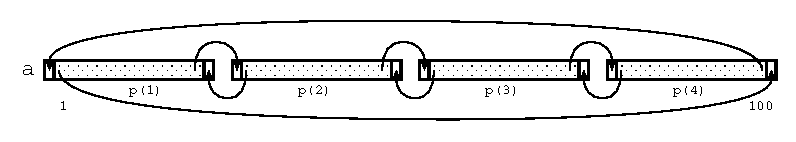
\includegraphics[width=0.9\hsize]{figs/fig3.2.eps}
\end{center}
\caption{Example of Periodic Shadow Reflection}
\label{fig3.2}
\end{myfigure}

The {\tt shadow} directive instructs to allocate ``periodic'' shadow
areas of the array {\tt a}.
The {\tt reflect} construct updates ``periodically'' the shadow area of
{\tt a} (Figure \ref{fig3.2}). A periodic shadow at the lower
bound on the node {\tt p(1)} is updated with the value of {\tt a(100)}
and that at the upper bound on {\tt p(4)} with the value of {\tt a(1)}.


\subsection{{\tt gmove} Construct}

\subsubsection*{Synopsis}

%The {\tt \Directive{gmove}} construct copies the data of a
%distributed array in the global view. 

The {\tt \Directive{gmove}} construct allows an assignment statement,
which may cause communication, to be executed possibly in parallel by
the executing nodes.

\subsubsection*{Syntax}
\Syntax{gmove}

\begin{tabular}{ll}
\verb![F]! & \verb|!$xmp| {\tt gmove} {\openb}{\tt in} $\vert$ {\tt
 out}{\closeb} {\openb}{\tt async (} {\it async-id} {\tt )}{\closeb}\\
% {\it dest} {\tt =} {\it source} \\
\verb![C]! & \verb|#pragma xmp| {\tt gmove} {\openb}{\tt in} $\vert$ {\tt
     out}{\closeb} {\openb}{\tt async (} {\it async-id} {\tt )}{\closeb}\\
% {\it dest} {\tt =} {\it source} \\
\end{tabular}

\subsubsection*{Description}

This construct copies the value of the right-hand side (rhs) variable
into the left-hand side (lhs) of the associated assignment statement,
which may require communication between nodes in the executing node
set. Such communication is detected, scheduled, and performed by the
XcalableMP runtime system.

%This construct executes a copy operation of the global data array object
%distributed into nodes.
%This directive is followed by the assignment
%statement of the scalar value and array sections.
%The assignment may require communication between nodes.

%Note that, in {\XMP}, the {\C} language is extended to support array
%section notation in order to support an assignment of array objects.

%The assignment statement must have one of the following patterns:
%
%\begin{itemize}
%\item  Scalar assignment. For example:
%
%\begin{tabular}{lll}
%\hspace{0.5cm} & {\tt s1 = s2} & ! {\tt s1} and {\tt s2} is a scalar
%variable \\ 
%& {\tt a(3) = b(i, j)} & ! {\tt a} and {\tt b} are arrays. \\
%\end{tabular}
%
%\item Array assignment. The left-hand-side variable must be either an
%      array name, an array section, or a scalar object. For example:
%
%\begin{tabular}{lll}
%\hspace{0.5cm} & {\tt a = b} & ! {\tt a} and {\tt b} are arrays \\
% & {\tt a(1:10) = b(n:n+9, k)} & ! lhs and rhs are array sections \\
% & {\tt a(1:10) = s2} & ! lhs is an array section and rhs is a
% scalar variable \\
% & {\tt a(1:10) = b(i, j)} & ! lhs is an array section and rhs is a
% scalar object \\
%\end{tabular}
%\end{itemize}

%The {\tt gmove} construct must be executed by all of the executing
%nodes. The value of scalar objects, the index value, and the range
%value of the array section in the assignment statement must be the same in
%every node executing this directive.

There are three operating modes of the {\tt gmove} construct:

\begin{itemize}
 \item {\bf collective mode}

       When neither the {\tt in} nor the {\tt out} clause is specified,
       the copy operation is performed collectively and cause an
       implicit synchronization after it among the executing node set.

%In this case, all elements in both the source array and the target array
%must be distributed onto the executing node set.
%If the object on the right-hand side is a local
%object, then the value of the local object must be the same.
%
%In this case, the assignment is performed locally, where the object on
%the left-hand side is distributed.
%
%If the object on the left-hand side is a local object
%and the object on the right-hand side is global, then this operation
%performs broadcast operation.

 \item {\bf in mode}

       When the {\tt in} clause is specified, the rhs data of the
       assignment, whole or parts of which may reside outside the
       executing node set, can be transferred from its owner nodes to
       the executing nodes by this construct.

       If the {\tt async} clause is not specified, then the construct is
       ``synchronous'' and it is guaranteed that the lhs data
       can be read and overwritten and all of the operations of the
       construct on the owner nodes and the executing node
       are completed when returning from the construct;
       otherwise, the construct is ``asynchronous'' and it is not
       guaranteed that until returning from the associating {\tt
       wait\_async} construct (Section \ref{subsec:wait_async
       Construct}).

 \item {\bf out mode}

       When the {\tt out} clause is specified, the lhs data of the
       assignment, whole or parts of which may reside outside the 
       executing node set, can be transferred from the executing nodes
       to its owner nodes by this construct.

       If the {\tt async} clause is not specified, then the construct is
       ``synchronous'' and it is guaranteed that the rhs data
       can be overwritten and all of the operations of the construct on
       the owner nodes and the executing node are
       completed when returning from the construct; otherwise, the
       construct is ``asynchronous'' and it is not guaranteed that until
       returning from the associating {\tt wait\_async} construct
       (Section \ref{subsec:wait_async Construct}).

\end{itemize}

%Note that, in these cases, no synchronization is implied and it is not
%ensured that the copy operation is completed. Thus, if a synchronization
%between the executing nodes and the owner nodes is required, the
%programmer must specify it explicitly by using a {\tt barrier} construct
%or a pair of a {\tt post} and an {\tt wait} construct.

%When an {\tt in} clause is specified, then the node that owns the
%element of the object on the left-hand side obtains the data on the
%right-hand side by the remote copy (get) operation.
%Therefore, the object on the left-hand side must be distributed onto
%the executing node set.
%
%When an {\tt out} clause is specified, then the node that owns the element
%of the object on the right-hand side places the data on the left-hand
%side by the remote copy (put) operation.
%Therefore, the object on the
%right-hand side must be distributed onto the executing node set.

%If no option is specified, then the copy can be performed by two-side
%communication. In this case, the receiver side waits for the sender side,
%resulting in implicit synchronization. 

%If an {\tt in} or {\tt out} clause is specified, then the
%copy operation should be performed by one-side communication for remote
%memory access. Thus, no synchronization is implied. If
%synchronization between reader and writer is required, then the programmer
%must perform synchronization explicitly by a {\tt barrier} construct. If
%the reader and the writer do not belong to the same executing node set,
%then point-to-point synchronization by {\tt post-wait} directive can be used.

When the {\tt async} clause is specified, the statements following this
construct may be executed before the operation is complete.

\subsubsection*{Restrictions}

\begin{itemize}
 \item The {\tt gmove} construct must be followed by (i.e. associated
       with) a simple assignment statement that contains neither
       arithmetic operations nor function calls.
 \item The {\tt gmove} construct is global, which means that it must be
       executed by all of the executing nodes, and each local variable
       referenced in the construct must have the same value among all of
       them.
 \item If the {\tt gmove} construct is in {\it collective} mode, then
       all elements of the distributed arrays appearing in both the
       lhs and the rhs of the associated assignment
       statement must reside in the executing node set.
 \item If the {\tt gmove} construct is in {\it in} mode, then
       all elements of the distributed array appearing in the lhs of the
       associated assignment statement must reside in the executing node
       set.
 \item If the {\tt gmove} construct is in {\it out} mode, then
       all elements of the distributed array appearing in the rhs of the
       associated assignment statement must reside in the executing node
       set.
 \item {\it async-id} must be an expression of type default integer, in
       {\XMPF}, or type {\tt int}, in {\XMPC}.
\end{itemize}

\subsubsection*{Examples}
\begin{description}
\item[Example 1: Array assignment]
\Example{gmove}

If both the lhs and the rhs are distributed
arrays, then the copy operation is performed by all-to-all
communication. If the lhs is a replicated array, this copy
is performed by multi-cast communication. If the rhs is a
replicated array, then no communication is required.

\vspace{0.5cm}

\begin{minipage}{0.45\hsize}
\begin{center}
\begin{XFexample}
!$xmp gmove
      a(:,1:N) = b(:,3,0:N-1)
\end{XFexample}
\end{center}
\end{minipage}
\begin{minipage}{0.45\hsize}
\begin{center}
\begin{XCexampleR}
#pragma xmp gmove
      a[1:N][:] = b[0:N][3][:];
\end{XCexampleR}
\end{center}
\end{minipage}
\vspace{1cm}

\item[Example 2: Scalar assignment to an array] 

When the rhs is an element of a distributed array, the copy
is performed by broadcast communication from the owner of the element. If 
the rhs is a replicated array, then no communication is required.

\vspace{0.5cm}

\begin{minipage}{0.45\hsize}
\begin{center}
\begin{XFexample}
!$xmp gmove
      a(:,1:N) = c(k)
\end{XFexample}
\end{center}
\end{minipage}
\begin{minipage}{0.45\hsize}
\begin{center}
\begin{XCexampleR}
#pragma xmp gmove
      a[1:N][:] = c[k]
\end{XCexampleR}
\end{center}
\end{minipage}
\vspace{1cm}

\item[Example 3: in mode assignment]

	   Since {\tt b(3)} referenced in the rhs of the
	   {\tt gmove} construct does not reside in the executing node
	   set ({\tt p(1:2)}), the construct is executed in in
	   mode. Thus, {\tt b(3)} is transferred from its owner node
	   {\tt p(3)} to the executing node set.

	   It is not guaranteed until {\tt p(1:2)} returns from the
	   construct that any node can read and overwrite {\tt a(1:2)}
	   and any relevant operations on {\tt p(1:2)} and {\tt p(3)}
	   are completed.

\vspace{0.5cm}

\begin{XFexample}
!$xmp nodes p(4)
!$xmp template t(4)
!$xmp distribute t(block) onto p

      real a(4), b(4)
!$xmp align (i) with t(i) : a, b
      ...
!$xmp task on p(1:2)
      ...
!$xmp gmove in
      a(1:2) = b(2:3)
      ...
!$xmp end task
\end{XFexample}

%$

\end{description}

\subsection{{\tt barrier} Construct}

\subsubsection*{Synopsis}

The {\tt \Directive{barrier}} construct specifies an explicit barrier
at the point at which the construct appears. 

\subsubsection*{Syntax}
\Syntax{barrier}

\begin{tabular}{ll}
\verb![F]! & \verb|!$xmp| {\tt barrier} {\openb}{\tt on} {\it nodes-ref}
 $\vert${\it template-ref}{\closeb} \\
\verb![C]! & \verb|#pragma xmp| {\tt barrier} {\openb}{\tt on} {\it
     nodes-ref} $\vert$ {\it template-ref}{\closeb} \\
\end{tabular}

\subsubsection*{Description}

The barrier operation is performed among the node set specified by
the {\tt on} clause. If no {\tt on} clause is specified, then it is
assumed that the current executing node set is specified in it.

Note that an {\tt on} clause may represent multiple node sets. In such a
case, a barrier operation is performed in each node set.

%The barrier construct also has the function of ensuring that all of the
%remote copy operations that are invoked by gmove in/out constructs
%executed by the node set specified by the {\tt on} clause are finished.

\subsubsection*{Restriction}

\begin{itemize}
\item The node set specified by the {\tt on} clause must be a subset of the
      executing node set.  
\end{itemize}


\subsection{{\tt reduction} Construct}

\subsubsection*{Synopsis}

The {\tt \Directive{reduction}} construct performs a reduction
operation among nodes. 

\subsubsection*{Syntax}
\Syntax{reduction}

\begin{tabular}{ll}
\verb![F]! & \verb|!$xmp| {\tt reduction (} {\it reduction-kind} {\it
  :} {\it variable} {\openb}, {\it variable} {\closeb}... {\tt )}\\
 & \hspace{6cm} {\openb}{\tt on} {\it node-ref} $\vert$ {\it
     template-ref}{\closeb} {\openb}{\tt async (} {\it async-id} {\tt
     )}{\closeb} \\
\end{tabular}

\vspace{0.5cm}

where {\it reduction-kind} is one of:

\begin{tabular}{ll}
 \hspace{0.5cm} & {\tt +} \\
 & {\tt *} \\
 & {\tt -} \\
 & {\tt .and.} \\
 & {\tt .or.} \\
 & {\tt .eqv.} \\
 & {\tt .neqv.} \\
 & {\tt max} \\
 & {\tt min} \\
 & {\tt iand} \\
 & {\tt ior} \\
 & {\tt ieor} \\
\end{tabular}

\vspace{0.5cm}

\begin{tabular}{ll}
 \hspace{-\parindent}
 \verb![C]! & \verb|#pragma xmp| {\tt reduction (} {\it reduction-kind} {\it
  :} {\it variable} {\openb}, {\it variable} {\closeb}... {\tt )}\\
 & \hspace{6cm} {\openb}{\tt on} {\it node-ref} $\vert$ {\it
     template-ref}{\closeb} {\openb}{\tt async (} {\it async-id} {\tt
     )}{\closeb} \\
\end{tabular}

\vspace{0.5cm}

where {\it reduction-kind} is one of:

\begin{tabular}{ll}
 \hspace{0.5cm} & {\tt +} \\
 & {\tt *} \\
 & {\tt -} \\
 & {\verb|&|} \\
 & {\tt |} \\
 & {\verb|^|} \\
 & {\verb|&&|} \\
 & {\tt ||} \\
 & {\tt max} \\
 & {\tt min} \\
\end{tabular}

\subsubsection*{Description}

The {\tt reduction} construct performs a type of
% modified by Sakagami,H. 09/11/13                                            
reduction operation specified by {\it reduction-kind} for the specified
local variables among the node set specified by the {\tt on}
clause and sets the reduction results to the variables on each of the
nodes.
%
Note that some of the reduction operation ({\tt FIRSTMAX}, {\tt
FIRSTMIN}, {\tt LASTMAX}, and {\tt LASTMIN}) that could be specified in
the {\tt reduction} clause of the {\tt loop} directive cannot be
specified in the {\tt reduction} construct, because their semantics are
not defined in it.
%
The variable specified by {\it variable}, which is the target of the
reduction operation, is referred to as the ``\Term{reduction
variable}.'' After the reduction operation, the value of the
reduction variable becomes the same in every node that performs the
operation.

The reduction result is computed by combining the reduction variables on
all of the nodes using the reduction operator. The ordering of this
reduction is implementation-dependent.

When the {\tt async} clause is specified, the statements following this
construct may be executed before the operation is complete.

% inserted by Sakagami,H. 09/11/13 ----- start ----                            
When {\it template-ref} is specified in the {\tt on} clause, the operation
is performed in a node set that consists of nodes onto which the
specified template section is distributed.
Therefore, before the {\tt reduction} construct is executed, the
referenced template must be fixed.
%
%When {\it template-subscript} in the {\it template-ref} is ``*'', nodes
%in the corresponding dimension are ignored for the reduction operation.
%
%When {\it template-subscript} in the {\it template-ref} is {\it
%triplet}, nodes for all template elements in the corresponding dimension
%perform the reduction operation.

When {\it nodes-ref} is specified in the {\tt on} clause, the operation
is performed in the specified node set.
%Therefore, before the {\tt \Directive{reduction}} construct is executed,
%the referenced node set must be fixed.

When the {\tt on} clause is omitted, the operation is performed in the
executing node set.

Note that an {\tt on} clause may represent multiple node sets. In such a
case, a reduction operation is performed in each node set.

\subsubsection*{Restrictions}

\begin{itemize}
%\item {\it template-spec} appearing in {\it template-ref} must be either ``*'', ``\
%:'' or the range.
%\item If {\tt on} clause is omitted, the operation is done in the current execu\
%ting node.
 \item The variables specified by the sequence of {\it variable}'s must
       either not be aligned or be replicated among nodes of the node
       set specified by the {\tt on} clause.
 \item The {\tt reduction} construct is global, which means that it must
       be executed by all of the executing nodes, and each local variable
       referenced in the construct must have the same value among all of
       the executing nodes.
 \item {\it async-id} must be an expression of type default integer, in
       {\XMPF}, or type {\tt int}, in {\XMPC}.
 \item The node set specified by the {\tt on} clause must be a subset of the
       executing node set.
\end{itemize}
% inserted by Sakagami,H. 09/11/13 ----- end ---- 

\subsubsection*{Examples}
\Example{reduction}

\begin{description}
\item[Example 1]
\hspace{\hsize}
\begin{XFexample}
!$xmp reduction(+:s)
!$xmp reduction(max:aa) on t(*,:)
!$xmp reduction(min:bb) on p(10:30)
\end{XFexample}

% modified by Sakagami,H. 09/11/13                                             
%In the first example, the scalar variable {\tt s} is assumed to contain the 
%partial sum of the variable, and the reduction operation calculates the
%total sum of the variable. The total sum is stored in the variable in
%each node.
In the first line, the reduction operation calculates the sum of the
scalar variable {\tt s} in the executing node set and the result is
stored in the variable in each node.

% modified by Sakagami,H. 09/11/13                                             
The reduction operation in the second line computes the maximum value of
the variable {\tt aa} in each node set onto which each of the template
section specified by {\tt t(*,:)} is distributed.
%that consists of nodes associated with the
%range of the second dimension of template {\tt t}.

% modified by Sakagami,H. 09/11/13                
In the third line, the minimum value of the variable {\tt bb} in the node 
set specified by {\tt p(10:30)} is calculated. This example is
equivalent to the following code using the {\tt \Directive{task}} construct.

\begin{XFexample}
!$xmp task on p(10:30)
!$xmp reduction(min:bb)
!$xmp end task
\end{XFexample}

\item[Example 2]
\hspace{\hsize}
\begin{XFexample}
      dimension a(n,n), p(n), w(n)
!$xmp align a(i,j) with t(i,j)
!$xmp align p(i) with t(i,*)
!$xmp align a(j) with t(*,j)
      ...
!$xmp loop (j) on t(:,j)
      do j = 1, n
          sum = 0
!$xmp loop (i) on t(i,j) reduction(+:sum)
          do i = 1, n
              sum = sum + a(i,j) * p(i)
          end do
          w(j) = sum
      end do
\end{XFexample}

This code computes the matrix vector product,
% modified by Sakagami,H. 09/11/13
where a {\tt reduction} clause is specified for the {\tt \Directive{loop}}
construct of the inner loop. This is equivalent to the following code
snippet. 

\begin{XFexample}
!$xmp loop (j) on t(:,j)
      do j = 1, n
          sum = 0
!$xmp loop (i) on t(i,j) 
          do i = 1, n
              sum - sum + a(i,j) * p(i)
          end do
!$xmp reduction(+:sum) on t(1:n,j)
          w(j) = sum
      end do
\end{XFexample}

In these cases, the reduction operation on the scalar variable {\tt sum}
is performed for every iteration in the outer loop, which may cause a
large overhead.
% modified by Sakagami,H. 09/11/13
The {\tt reduction} clause cannot be specified for the {\tt
\Directive{loop}} construct of the outer loop to reduce this overhead,
%
%because the loop index of the outer loop ({\tt j}) is different from that 
%for the reduction operation ({\tt i}).
because the node set where the reduction operation specified by a {\tt
reduction} clause of a {\tt loop} construct is performed is determined
from its {\tt on} clause (see \ref{sub:loop_construct}) and
the {\tt on} clause of the outer {\tt loop} construct is different from
that of the inner one. 
%
However, this code can be modified with the {\tt \Directive{reduction}}
construct as follows: 

\begin{XFexample}
      dimension a(n,n), p(n), w(n)
!$xmp align a(i,j) with t(i,j)
!$xmp align p(i) with t(i,*)
!$xmp align a(j) with t(*,j)
      ...
!$xmp loop (j) on t(:,j)
      do j = 1, n
          sum = 0
!$xmp loop (i) on t(i,j) 
          do i = 1, n
              sum - sum + a(i,j) * p(i)
          end do
          w(j) = sum
      end do
!$xmp reduction(+:w) on t(1:n,*)
\end{XFexample}

This code performs a reduction operation on the array {\tt w} only once,
which may result in faster operation.  

\end{description}


\subsection{{\tt bcast} Construct}

\subsubsection*{Synopsis}

The {\tt \Directive{bcast}} construct performs broadcast communication
from one specified node.

\subsubsection*{Syntax}
\Syntax{bcast}

\begin{tabular}{ll}
 \verb![F]! & \verb|!$xmp| {\tt bcast} \verb|(| {\it variable} 
 {\openb}, {\it variable}{\closeb}... \verb|)|
 {\openb}{\tt from} {\it nodes-ref} $\vert$ {\it template-ref}{\closeb}\\
 & \hspace{6cm} {\openb}{\tt on} {\it nodes-ref}{\closeb} $\vert$ {\it
     template-ref}{\closeb}
 {\openb}{\tt async (} {\it async-id} {\tt )}{\closeb} \\

 \verb![C]! & \verb|#pragma xmp| {\tt bcast} \verb|(| {\it variable} 
 {\openb}, {\it variable}{\closeb}... \verb|)|
 {\openb}{\tt from} {\it nodes-ref}  $\vert$ {\it template-ref}{\closeb}\\
 & \hspace{6cm} {\openb}{\tt on} {\it nodes-ref} $\vert$ {\it
     template-ref}{\closeb}
 {\openb}{\tt async (} {\it async-id} {\tt )}{\closeb} \\

\end{tabular}

\subsubsection*{Description}

The values of the variables specified by the sequence of {\it
variable}'s (called {\it \Term{broadcast variables}}) are broadcasted 
from the node specified by the {\tt from} clause (called the
{\it \Term{source node}}) to each of the nodes in the node set specified
by the {\tt on} clause. After executing this construct,
the values of the broadcast variables become the same as those in the
source node.
%
If the {\tt from} clause is omitted, then the {\it first}
node, that is, the leading one in Fortran's array element order, of the
node set specified by the {\tt on} clause is assumed to be a source
node.
%
If the {\tt on} clause is omitted, then it is assumed that the current
executing node set is specified in it.

When the {\tt async} clause is specified, the statements following this
construct may be executed before the operation is complete.

\subsubsection*{Restrictions}

\begin{itemize}
 \item The variables specified by the sequence of {\it variable}'s must
       either not be aligned or be replicated among nodes of the node set
       specified by the {\tt on} clause.
 \item The {\tt bcast} construct is global, which means that it must be
       executed by all of the executing nodes, and each local variable
       referenced in the construct must have the same value among all of
       the executing nodes.
 \item {\it async-id} must be an expression of type default integer, in
       {\XMPF}, or type {\tt int}, in {\XMPC}.
 \item The node set specified by the {\tt on} clause must be a subset of the
       current executing node set.
 \item The source node specified by the {\tt from} clause must belong to
       the node set specified by the {\tt on} clause.
 \item The source node specified by the {\tt from} clause must be one node.
\end{itemize}


\subsection{{\tt wait\_async} Construct}
\label{subsec:wait_async Construct}

\subsubsection*{Synopsis}

The {\tt \Directive{wait\_async}} construct guarantees asynchronous
communications specified by {\it async-id}.

\subsubsection*{Syntax}
\Syntax{wait\_async}

\begin{tabular}{ll}
\verb![F]! & \verb|!$xmp| {\tt wait\_async ( {\it async-id} {\openb},
 {\it async-id} {\closeb}... )} \\
\verb![C]! & \verb|#pragma xmp| {\tt wait\_async ( {\it async-id} {\openb},
 {\it async-id} {\closeb}... )} \\
\end{tabular}

\subsubsection*{Description}

The {\tt \Directive{wait\_async}} construct blocks and therefore
statements after it are not executed until all of the asynchronous
communications specified by each of {\it async-id} are complete. 

\subsubsection*{Restrictions}

\begin{itemize}
 \item {\it async-id} must be an expression of type default integer, in
       {\XMPF}, or type {\tt int}, in {\XMPC}.
\item {\it async-id} must be associated with an asynchronous
      communication by the {\tt async} clause of a communication
      construct or an {\tt async} construct.
\item The {\tt wait\_async} construct is global, which means that it must
      be executed by all of the executing nodes, and each local variable
      referenced in the construct must have the same value among all of
      the executing nodes.
\item The executing node set of the {\tt wait\_async} construct must be
      the same as that of the global constructs that initiate the
      asynchronous communications specified by {\it async-id}.
%\item Every communication specified by each {\it async-id} must be
%      executed on the same executing node set.
\end{itemize}


\subsection{{\tt async} Clause}

\subsubsection*{Synopsis}

The {\tt async} clause of the {\tt reflect}, {\tt gmove}, {\tt
reduction} and {\tt bcast} construct allows the corresponding
communication to be performed asynchronously.

\subsubsection*{Description}

Communication corresponding to the construct with an {\tt async} clause
is performed asynchronously, that is, initiated but not completed,
and therefore statements following it may be executed before the
communication is complete.

\subsubsection*{Example}
\Example{wait\_async}

\begin{XFexample}
!$xmp reflect (a) async(1)
      S1
!$xmp wait_async(1)
      S2
\end{XFexample}

The {\tt reflect} construct on the first line matches
the {\tt wait} construct on the third line because both of their {\it
async\_id} evaluate to 1.
%
These constructs ensure that statements in {\tt S1} can be executed
before the {\tt reflect} communication is complete and no statement in
{\tt S2} is executed until the {\tt reflect} communication is
complete.

\cleardoublepage

%\chapter{Procedure call and data mapping for procedure argument}
\chapter{Procedure Interfaces}
\label{chap:procedure}
\index{procedure interface}

This chapter describes the procedure interfaces, that is, how
procedures are invoked and arguments are passed, in {\XMP}.

In order to achieve high composability of {\XMP} programs, it is one of
the most important requirement that {\XMP} procedures can invoke
procedures written in the base language with as a few restrictions as
possible.
%The procedure interfaces in {\XMP} is designed so as to
%satisfy the requirement.


\section{General Rule}

In {\XMP}, a procedure invocation itself is a local operation and does
not cause any communication or synchronization at runtime. Thus, a node
can invoke any procedure, whether written in {\XMP} or in the base
language, at any point of the execution.
%
There is no restriction on the characteristics of procedures invoked by
an {\XMP} procedure, except for a few ones on its argument, which is
explained below.

A local data in the actual or dummy argument list (referred to as a {\it
\Term{local actual argument}} and a {\it \Term{local dummy argument}},
respectively) are treated by the {\XMP} compiler in the same manner as
by the compiler of the base language.
%
This rule makes it possible that a local actual argument in a procedure
written in {\XMP} can be associated with a dummy argument of a procedure
written in the base language.

If both of an actual and its associating dummy arguments are coarrays,
they must be declared on the same node set.


\paragraph{Implementation.}

The {\XMP} compiler does not transform either local actual or dummy
arguments, so that the backend compiler of the base language can treat
them in its usual way.

\vspace{1.5zw}

\hspace{-1.2\parindent}
The rest of this chapter specifies how global data appearing as an
actual and a dummy argument list (referred to as a {\it \Term{global actual
argument}} and a {\it \Term{global dummy argument}}, respectively) are
processed by the {\XMP} compiler.


\section{Argument Passing Mechanism in {\XMP} Fortran}

%Any section (except for an element) of a global data may not be put in
%the actual argument list. Therefore only the name or an element of it
%may be put in the actual argument list.

Either of the following global data can be put in the actual argument list:

\begin{itemize}
 \item an array name;
 \item an array element; or
 \item an array section that satisfies both of the following two
       conditions:
       \begin{itemize}
	\item its subscript list is a list of zero or more colons
	      (``{\tt :}'') followed by zero or more {\it int-expr}'s;
	\item a subscript of the dimension having shadow is {\it
	      int-expr} unless it is the last dimension.
       \end{itemize}
\end{itemize}

There are two kinds of argument association for global data in {\XMP}
Fortran: one is {\it \Term{sequence association}}, which is for a global
dummy that is an explicit-shape or assumed-size array, and the other is
{\it \Term{descriptor association}}, which is for all other global dummy.


\subsection{Sequence Association of Global Data}
\index{sequence association}

The concept of sequence association in {\Fort} is extended for global
actual and dummy arguments in {\XMP} as follows.

If the actual argument is an array name or an array section that
satisfies the above conditions, it represents an element sequence
consisting of the elements of its local section in Fortran's array
element order on each node.
%
Also, if the actual argument is an element of a global data, it
represents an element sequence consisting of the corresponding element
in the local section and each element that follows it in array element
order on each node.

An global actual argument that represents an element sequence and
corresponds to a global dummy argument is sequence associated with
the the dummy argument if the dummy argument is an explicit-shape or
assumed-size array.
%
According to this (extended) sequence association rule, each element of
the element sequence represented by the global actual argument is
associated with the element of the local section of the global dummy
argument that has the same position in array element order.

Sequence association is the default rule of association for global
actual arguments and therefore is applied unless it is obvious from the
interface of the invoked procedure that the corresponding dummy argument
is neither an explicit-shape nor assumed-size array.


\paragraph{Implementation.}

In order to implement sequence association, the name, a section, or an
element of a global data appearing as an actual argument is treated by
the {\XMP} compiler as the base address of its local section on each
node, and the global data appearing as the corresponding dummy argument
is initialized at runtime so as to be composed of the local sections
each of which starts from the address received as the argument.
%
On a node that does not have the local section corresponding to the
actual argument, an unspecified value (e.g. null) is received.

Such implementation implies that in many cases, in order to associate
properly a global actual argument with the global dummy argument, their
mappings (including their shadow attributes) must be identical.


\subsubsection*{Examples}
\index{Example!{procedure interface}}

\begin{description}

\item[Example 1]

	   Both the actual argument {\tt a} and the dummy argument {\tt
	   x} are global explicit-shape arrays, and therefore {\tt
	   a} is sequence associated with {\tt x}.

	   It is the base address of the local section of {\tt a} that
	   passed between these subroutines on each node. Each the local
	   section of {\tt x} starts from the received address (Figure
	   \ref{fig5.1}).

\begin{XFexample}
      subroutine xmp_sub1
!$xmp nodes p(4)
!$xmp template t(100)
!$xmp distribute t(block) onto p
      real a(100)
!$xmp align a(i) with t(i)
!$xmp shadow a(1:1) 
      call xmp_sub2(a)
      end subroutine

      subroutine xmp_sub2(x)
!$xmp nodes p(4)
!$xmp template t(100)
!$xmp distribute t(block) onto p
      real x(100)
!$xmp align x(i) with t(i)
!$xmp shadow x(1:1) 
      ...
\end{XFexample}

\begin{myfigure}
 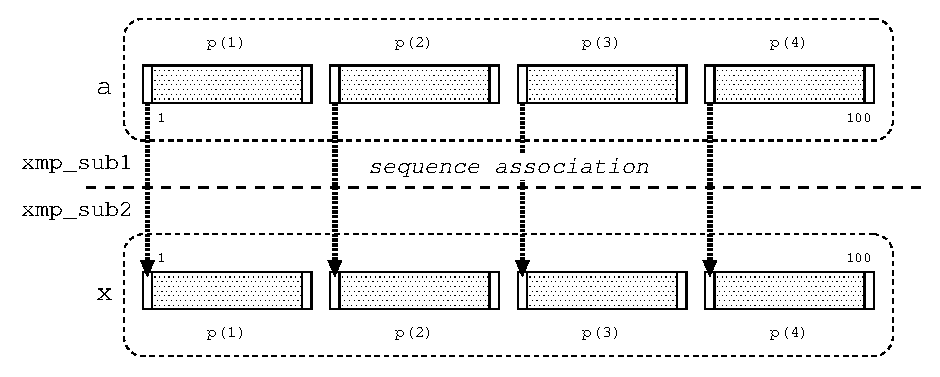
\includegraphics[scale=0.7]{figs/fig5.1.eps}
 \caption{Sequence Association with a Global Dummy Argument}
 \label{fig5.1}
\end{myfigure}

\item[Example 2]

	   The actual argument {\tt a} is a global explicit-shape array,
	   and the dummy argument {\tt x} is a local explicit-shape. 
	   Sequence association is applied also in this case.

	   The caller subroutine {\tt xmp\_sub1} passes the base address
	   of the local section of {\tt a} on each node, and the callee
	   {\tt f\_sub2} receives it and initializes {\tt x} with the
	   storage starting from it (Figure \ref{fig5.2}).

\begin{XFexample}
      subroutine xmp_sub1
!$xmp nodes p(4)
!$xmp template t(100)
!$xmp distribute t(block) onto p
      real a(100)
!$xmp align a(i) with t(i)
!$xmp shadow a(1:1) 
      n = 1 + 100/4 + 1
      call f_sub2(a,n)
      end subroutine
\end{XFexample}
\begin{Fexample}
      subroutine f_sub2(x,n)
      real x(n)
      ...
\end{Fexample}

\begin{myfigure}
 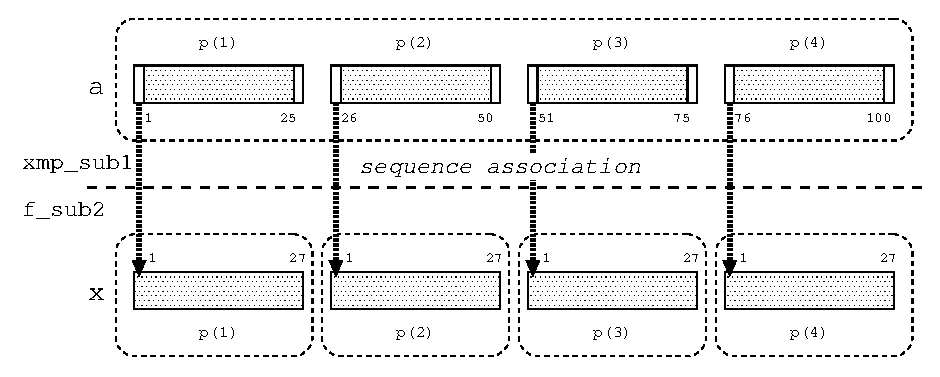
\includegraphics[scale=0.7]{figs/fig5.2.eps}
 \caption{Sequence Association with a Local Dummy Argument}
 \label{fig5.2}
\end{myfigure}

\item[Example 3]

	   The actual argument {\tt a(:,1)} is a contiguous section of
	   the global data, and the dummy argument {\tt x} is a local
	   explicit-shape array. Sequence association is applied 
	   in this case, but only the node {\tt p(1)} owns the section.
	   Hence, {\tt f\_sub2} is invoked only by {\tt p(1)} (Figure
	   \ref{fig5.25}).

\begin{XFexample}
      subroutine xmp_sub1
!$xmp nodes p(4)
!$xmp template t(100,100)
!$xmp distribute t(*,block) onto p
      real a(100,100)
!$xmp align a(i,j) with t(i,j)
!$xmp shadow a(0,1:1)
      n = 100
!$xmp task on p(1)
      call f_sub2(a(:,1),n)
!$xmp end task
      end subroutine
\end{XFexample}
%
\begin{Fexample}
      subroutine f_sub2(x,n)
      real x(n)
      ...
\end{Fexample}

\clearpage

\begin{myfigure}
 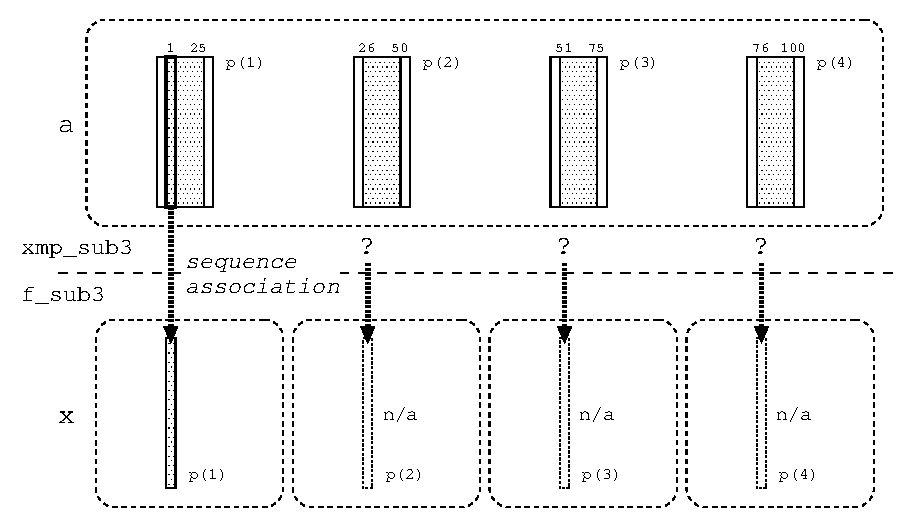
\includegraphics[scale=0.7]{figs/fig5.25.eps}
 \caption{Sequence Association of a Section of a Global Data as an
 Actual Argument with a Local Dummy Argument}
 \label{fig5.25}
\end{myfigure}

\item[Example 4]

	   The actual argument {\tt a(1)} is an element of the global
	   data, and the dummy argument {\tt x} is a local
	   explicit-shape array. Sequence association is applied 
	   in this case, but only the node {\tt p(1)} owns the element.
	   Hence, {\tt f\_sub2} is invoked only by {\tt p(1)}(Figure
	   \ref{fig5.3}).

\begin{XFexample}
      subroutine xmp_sub1
!$xmp nodes p(4)
!$xmp template t(100)
!$xmp distribute t(block) onto p
      real a(100)
!$xmp align a(i) with t(i)
!$xmp shadow a(1:1)
      n = 100/4
!$xmp task on p(1)
      call f_sub2(a(1),n)
!$xmp end task
      end subroutine
\end{XFexample}
%
\begin{Fexample}
      subroutine f_sub2(x,n)
      real x(n)
      ...
\end{Fexample}

\begin{myfigure}
 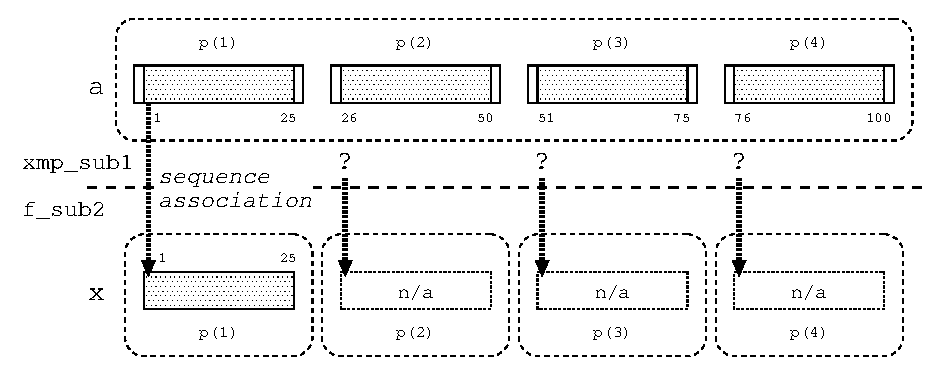
\includegraphics[scale=0.7]{figs/fig5.3.eps}
 \caption{Sequence Association of an Element of a Global Data as an
 Actual Argument with a Local Dummy Argument}
 \label{fig5.3}
\end{myfigure}

\item[Example 5]

	   Even if either the global actual or dummy argument has a full
	   shadow, the sequence association rule is the same in
	   principle. Hence, the base address of the local section of
	   {\tt a} is passed between these subroutines on each node, and
	   each the local section of {\tt x} starts from the received
	   address (Figure \ref{fig5.4}).

\begin{myfigure}
 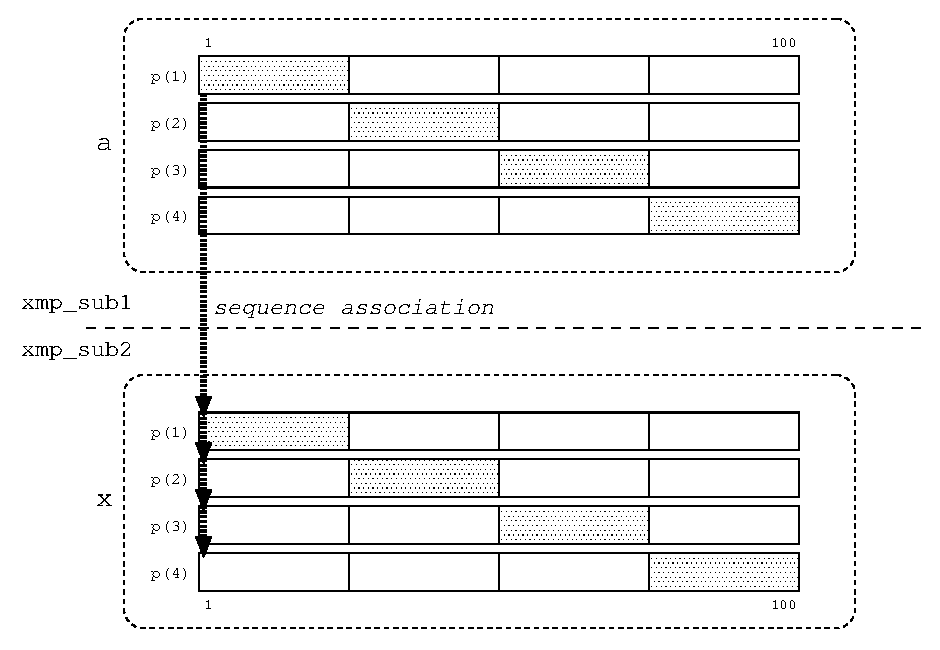
\includegraphics[scale=0.7]{figs/fig5.4.eps}
 \caption{Sequence Association with a Global Dummy Argument that Has
 Full Shadow}
 \label{fig5.4}
\end{myfigure}

\end{description}


\subsection{Descriptor Association of Global Data}
\index{descriptor association}

When the actual argument is a global data and it is obvious from the
interface of the invoked procedure that the corresponding dummy argument
is neither an explicit-shape nor assumed-size array, the actual
argument is {\it descriptor associated} with the dummy
argument. According to the descriptor association rule, the dummy
argument inherits its shape and storage from the actual argument.

\paragraph{Implementation.}

In order to implement the descriptor association, a global actual
argument is treated by the {\XMP} compiler:

\begin{itemize}
 \item as if it were the {\it global-data descriptor} of the actual array, 
       which is an internal data structure managed by the {\XMP} runtime
       system to hold information on a global data (see \ref{subsec:
       xmp_desc_of}), if the dummy is a global data; or
 \item as it is an array representing the local section of the actual
       array, which is to be processed by the backend Fortran compiler
       in the same manner as usual data, if the dummy is a local data.
\end{itemize}

For the first case, a global dummy is initialized at runtime with a copy
of the global-data descriptor received.

When an actual argument is descriptor associated with the dummy argument
and their mappings are not identical, the {\XMP} runtime system may
detect and report the error.

\subsubsection*{Examples}
\index{Example!{procedure interface}}

\begin{description}

\item[Example 1]

	   There is the explicit interface of the subroutine
	   {\tt xmp\_sub2} specified by an interface block in the
	   subroutine {\tt xmp\_sub1}, from which it is found that the
	   dummy argument {\tt x} is a global assumed-shape
	   array. Therefore the global actual argument {\tt a} is
	   descriptor associated with the global dummy argument {\tt
	   x}.

	   It is the global-data descriptor of {\tt a} that passed
	   between these subroutines. The dummy argument {\tt x} is
	   initialized by the {\XMP} runtime system on the basis of the
	   information extracted from the descriptor received (Figure
	   \ref{fig5.5}).

\begin{XFexample}
      subroutine xmp_sub1

!$xmp nodes p(4)
!$xmp template t(100)
!$xmp distribute t(block) onto p
      real a(100)
!$xmp align a(i) with t(i)
!$xmp shadow a(1:1)

      interface
      subroutine xmp_sub2(x)
!$xmp nodes p(4)
!$xmp template t(100)
!$xmp distribute t(block) onto p
      real x(:)
!$xmp align x(i) with t(i)
!$xmp shadow a(1:1)
      end subroutine xmp_sub2
      end interface

      call xmp_sub2(a)

      end subroutine

      subroutine xmp_sub2(x)
!$xmp nodes p(4)
!$xmp template t(100)
!$xmp distribute t(block) onto p
      real x(:)
!$xmp align x(i) with t(i)
!$xmp shadow a(1:1)
      ...
\end{XFexample}

\begin{myfigure}
 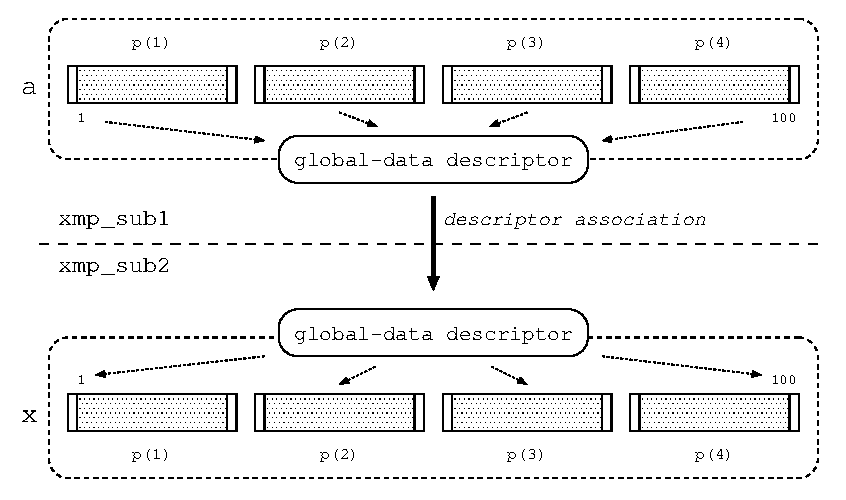
\includegraphics[scale=0.7]{figs/fig5.5.eps}
 \caption{Descriptor Association with a Global Dummy Argument}
 \label{fig5.5}
\end{myfigure}

\item[Example 2]

	   There is the explicit interface of the subroutine
	   {\tt f\_sub2}, which is written in {\Fort},
	   specified by an interface block in the subroutine {\tt
	   xmp\_sub1}, and the dummy argument {\tt x} is a local
	   (i.e. non-mapped) assumed-shape array. Therefore the global
	   actual argument {\tt a} is descriptor associated with the
	   local dummy argument {\tt x}.

	   The global actual argument is replaced with its local section
	   by the {\XMP} compiler and the association of the local
	   section with the dummy argument is to be processed by the
	   backend Fortran compiler in the same manner as usual data 
	   (Figure \ref{fig5.6}).

\begin{XFexample}
      subroutine xmp_sub1

!$xmp nodes p(4)
!$xmp template t(100)
!$xmp distribute t(block) onto p
      real a(100)
!$xmp align a(i) with t(i)
!$xmp shadow a(1:1) 

      interface
      subroutine f_sub2(x)
      real x(:)
      end subroutine f_sub2
      end interface

      call f_sub2(a)

      end subroutine
\end{XFexample}
\begin{Fexample}
      subroutine f_sub2(x)
      real x(:)
      ...
\end{Fexample}

\begin{myfigure}
 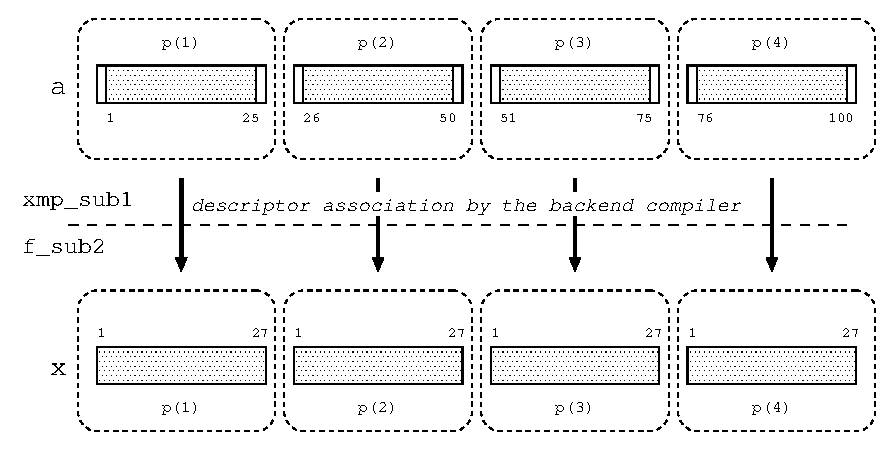
\includegraphics[scale=0.7]{figs/fig5.6.eps}
 \caption{Descriptor Association with a Local Dummy Argument}
 \label{fig5.6}
\end{myfigure}

\end{description}


\section{Argument Passing Mechanism in {\XMP} C}

When an actual argument is a global data, it is passed by the address
of its local section.
%
When a dummy argument is a global data, an address is received and
used as the base address of each of its local section.


\paragraph{Implementation.}

The name of a global data appearing as an actual argument is
treated by the {\XMP} compiler as the pointer to the first element of
its local section on each node.
%
On a node onto which no part of the global data is mapped, the pointer
is set to an unspecified value (e.g. null).
%
Note that an element of a global data in the actual argument list is
treated in the same manner as those in other usual statements because an
array element is passed by value as in C.

The name of a global data appearing as a dummy argument is
treated by the {\XMP} compiler as the pointer to the first element of
its local section on each node.
%
As a result, it is initialized at runtime so as to be
composed of the local sections on the executing nodes.

Such implementation implies that in many cases, in order to pass
properly a global actual argument to the corresponding global dummy 
argument, their mappings (including their shadow attributes) must be
identical.

\subsubsection*{Examples}
%\index{Example!{procedure interface}}

\begin{description}

\item[Example 1]

	   The global actual argument {\tt a} is treated by the {\XMP}
	   compiler as the pointer to the first element of its local
	   section, which is passed to the callee, on each node.

	   The global dummy argument {\tt x} is initialized so that each
	   of its local section starts from the address held by the
	   received pointer (Figure \ref{fig5.7}).

\begin{XCexample}
void xmp_func1()
{
#pragma xmp nodes p(4)
#pragma xmp template t(0:99)
#pragma xmp distribute t(block) onto p
  float a[100];
#pragma xmp align a[i] with t(i)
#pragma xmp shadow a[1:1]

  xmp_func2(a);
}

void xmp_func2(float x[100])
{
#pragma xmp nodes p(4)
#pragma xmp template t(0:99)
#pragma xmp distribute t(block) onto p
#pragma xmp align x[i] with t(i)
#pragma xmp shadow a[1:1]
  ...
\end{XCexample}

\begin{myfigure}
 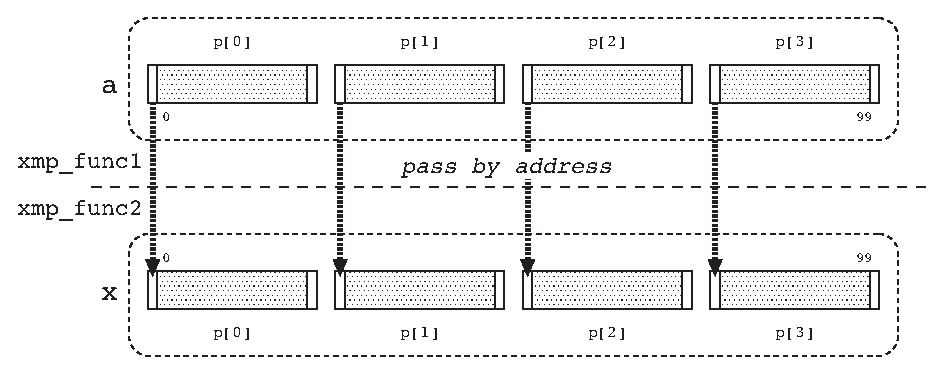
\includegraphics[scale=0.7]{figs/fig5.7.eps}
 \caption{Passing to a Global Dummy Argument}
 \label{fig5.7}
\end{myfigure}

\item[Example 2]

	   The global actual argument {\tt a} is treated by the {\XMP}
	   compiler as the pointer to the first element of its local
	   section, which is passed to the callee, on each node.

	   The local dummy argument {\tt x} on each node starts from the 
	   address held by the received pointer (Figure \ref{fig5.8}).

\begin{XCexample}
void xmp_func1()
{
#pragma xmp nodes p(4)
#pragma xmp template t(0:99)
#pragma xmp distribute t(block) onto p
  float a[100];
#pragma xmp align a[i] with t(i)
#pragma xmp shadow a[1:1]

  c_func2(a);
}
\end{XCexample}
\begin{Cexample}
void c_func2(float x[27])
{
  ...
\end{Cexample}

\begin{myfigure}
 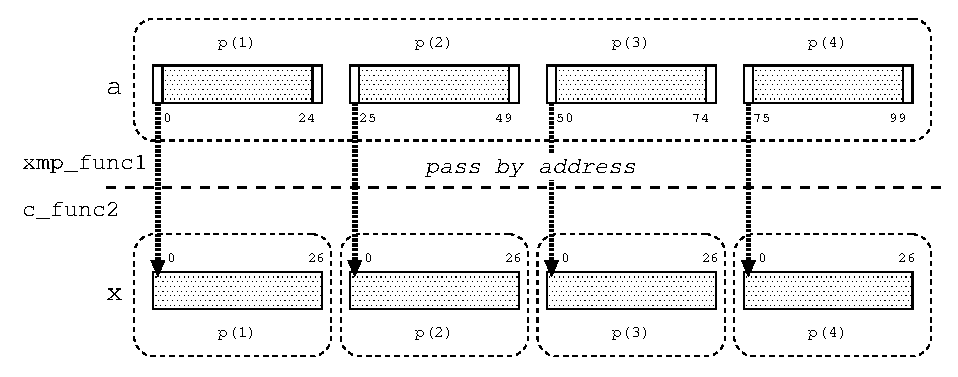
\includegraphics[scale=0.7]{figs/fig5.8.eps}
 \caption{Passing to a Local Dummy Argument}
 \label{fig5.8}
\end{myfigure}

\item[Example 3]

	   The actual argument {\tt a[0]} is an element of the global
	   data and the dummy argument {\tt x} is a scalar, in which
	   case the normal argument-passing rule of {\C} for variables
	   of a basic type (i.e. ``pass-by-value'') is applied. However,
	   only the node {\tt p(1)} owns the element.
	   Hence, {\tt c\_func2} is invoked only by {\tt p(1)} (Figure
	   \ref{fig5.9}).

\begin{XCexample}
void xmp_func1()
{
#pragma xmp nodes p(4)
#pragma xmp template t(0:99)
#pragma xmp distribute t(block) onto p
  float a[100];
#pragma xmp align a[i] with t(i)
#pragma xmp shadow a[1:1]

#pragma xmp task on p(1)
  c_func2(a[0]);
}
\end{XCexample}
\begin{Cexample}
void c_func2(float x)
{
  ...
\end{Cexample}

\begin{myfigure}
 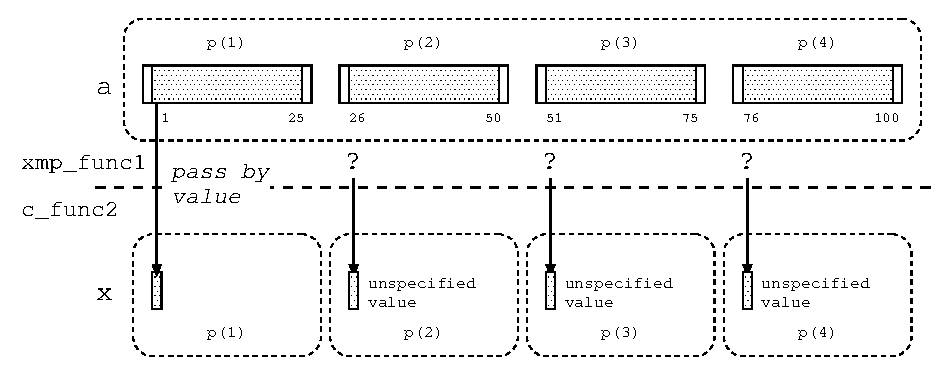
\includegraphics[scale=0.7]{figs/fig5.9.eps}
 \caption{Passing an Element of a Global Data as an Actual Argument to a
 Local Dummy Argument}
 \label{fig5.9}
\end{myfigure}

\end{description}

\cleardoublepage

\chapter{Intrinsic and Library Procedures}
\label{chap:Intrinsic and library procedures}

This specification defines various procedures for system inquiry,
synchronization, computations, etc. The procedures are provided as
intrinsic procedures in {\XMPF} and library procedures in {\XMPC}.

\section{System Inquiry Procedures}

\begin{itemize}
 \item {\tt xmp\_desc\_of}
 \item {\tt xmp\_all\_node\_num}
 \item {\tt xmp\_all\_num\_nodes}
 \item {\tt xmp\_node\_num}
 \item {\tt xmp\_num\_nodes}
% \item {\tt xmp\_mpi\_comm}
 \item {\tt xmp\_wtime}
 \item {\tt xmp\_wtick}
\end{itemize}

\subsection{\tt xmp\_desc\_of}
\label{subsec: xmp_desc_of}
\Intrinsic{xmp\_desc\_of}
\index{descriptor-of operator}
\index{xmp\_desc\_of@{\tt xmp\_desc\_of}}

\subsubsection*{Format}

\begin{tabular}{lll}

\verb![F]!&  {\tt integer(kind=xmp\_desc\_kind)}& {\tt xmp\_desc\_of(xmp\_entity)}\\

\verb![C]!&  {\tt xmp\_desc\_t}& {\tt xmp\_desc\_of(xmp\_entity)}

\end{tabular}

\vspace{0.3cm}

Note that {\tt xmp\_desc\_of} is an intrinsic function in {\XMPF} or
a built-in operator in {\XMPC}.

\subsubsection*{Synopsis}

%    A {\tt xmp\_desc\_of} is an input argument of query functions.
%    When Query functions get descriptor information of array
%    from XMP compiler, they must set a {\tt xmp\_desc\_of} as an
%    input argument.

{\tt xmp\_desc\_of} returns, in {\XMPF}, or is evaluated to, in {\XMPC},
a descriptor to retrieve informations of the specified global array,
template, or node array. The resulting descriptor can be used as an
input argument of the inquiry procedures which is described in appendix
\ref{chap:Interface to Numerical Libraries}.

The kind type parameter of the type of the descriptor, {\tt
xmp\_desc\_kind}, in {\XMPF} is implementation-dependent, and defined in
a Fortran module named {\tt xmp\_lib} or a Fortran {\tt include} file
named {\tt xmp\_lib.h}.

The type of the descriptor, {\tt xmp\_desc\_t}, in {\XMPC} is
implementation-dependent, and defined in a header file named {\tt xmp.h}
in {\XMPC}.

%The type of the descriptor, {\tt xmp\_desc\_t}, is
%implementation-dependent, and defined in a Fortran module named {\tt
%xmp\_lib} or a Fortran {\tt include} file named {\tt xmp\_lib.h} in
%{\XMPF}, or a header file named {\tt xmp.h} in {\XMPC}.

\subsubsection*{Arguments}

The argument or operand {\tt xmp\_entity} is the name of either a global
array, a template or a node array.

%   The argument of {\tt xmp\_desc\_of} is an {\it array-name}, a {\it template-name}, or a {\it nodes-name}.
%   In the case of {\it array-name}, return value d is a pointer to
%   be able to access array descriptor information.
%   In the case of {\it template-name}, return value d is a pointer to
%   be able to access template descriptor information.
%   In the case of {\it nodes-name}, return value d is a pointer to
%   be able to access node descriptor information.
%   If the argument of {\tt xmp\_desc\_of} is a local data, it is unchanged.


\subsection{\tt xmp\_all\_node\_num}
\Intrinsic{xmp\_all\_node\_num}

\subsubsection*{Format}

\begin{tabular}{lll}

\verb![F]!&  {\tt integer function}& {\tt xmp\_all\_node\_num()}\\

\verb![C]!&  {\tt int}& {\tt xmp\_all\_node\_num(void)}

\end{tabular}

\subsubsection*{Synopsis}

     The {\tt xmp\_all\_node\_num} routine returns the node number,
     within the primary node set, of the node that calls {\tt
     xmp\_all\_node\_num}.

\subsubsection*{Arguments}

    none.


\subsection{\tt xmp\_all\_num\_nodes}
\Intrinsic{xmp\_all\_num\_nodes}

\subsubsection*{Format}

\begin{tabular}{lll}

\verb![F]!&  {\tt integer function}& {\tt xmp\_all\_num\_nodes()}\\

\verb![C]!&  {\tt int}& {\tt xmp\_all\_num\_nodes(void)}

\end{tabular}

\subsubsection*{Synopsis}

     The {\tt xmp\_all\_num\_nodes} routine returns the number of nodes
     in the entire node set.

\subsubsection*{Arguments}

    none.


\subsection{\tt xmp\_node\_num}
\Intrinsic{xmp\_node\_num}

\subsubsection*{Format}

\begin{tabular}{lll}

\verb![F]!&  {\tt integer function}& {\tt xmp\_node\_num()}\\

\verb![C]!&  {\tt int}& {\tt xmp\_node\_num(void)}

\end{tabular}

\subsubsection*{Synopsis}

     The {\tt xmp\_node\_num} routine returns the node number,
     within the current executing node set, of the node that calls {\tt
     xmp\_node\_num}.

\subsubsection*{Arguments}

none.


\subsection{\tt xmp\_num\_nodes}
\Intrinsic{xmp\_num\_nodes}

\subsubsection*{Format}

\begin{tabular}{lll}

\verb![F]!&  {\tt integer function}& {\tt xmp\_num\_nodes()}\\

\verb![C]!&  {\tt int}& {\tt xmp\_num\_nodes(void)}

\end{tabular}

\subsubsection*{Synopsis}

     The {\tt xmp\_num\_nodes} routine returns the number of the
     executing nodes.

\subsubsection*{Arguments}

none.

%\subsection{\tt xmp\_mpi\_comm}
%
%\subsubsection*{Format}
%
%\begin{tabular}{lll}
%
%\verb![F]!&  {\tt integer function}& {\tt xmp\_mpi\_comm({\it nodes-name})}\\
%
%\verb![C]!&  {\tt int}& {\tt xmp\_mpi\_comm({\it nodes-name})}
%
%\end{tabular}
%
%\subsubsection*{Synopsis}
%     The {\tt xmp\_mpi\_comm} routine returns the integer value with associated communicator
%     to which {\it nodes-name} belongs. If non {\it nodes-name}, {\tt xmp\_mpi\_comm} returns 
%     the value of MPI\_Comm\_World.
%
%\subsubsection*{Arguments}
%    The argument of {\tt xmp\_mpi\_comm} is a {\it nodes-name} of the executing node set.
%
%

\subsection{\tt xmp\_wtime}
\Intrinsic{xmp\_wtime}

\subsubsection*{Format}

\begin{tabular}{lll}

\verb![F]!&  {\tt double precision function}& {\tt xmp\_wtime()}\\

\verb![C]!&  {\tt double}& {\tt xmp\_wtime(void)}

\end{tabular}

\subsubsection*{Synopsis}
    The {\tt xmp\_wtime} routine returns elapsed wall clock time in seconds 
    since some time in the past. The ``time in the past'' is guaranteed
    not to change during the life of the process.
    There is no requirement that different nodes return ``the same time.''

\subsubsection*{Arguments}
    none.


\subsection{\tt xmp\_wtick}
\Intrinsic{xmp\_wtick}

\subsubsection*{Format}

\begin{tabular}{lll}

\verb![F]!&  {\tt double precision function}& {\tt xmp\_wtick()}\\

\verb![C]!&  {\tt double}& {\tt xmp\_wtick(void)}

\end{tabular}

\subsubsection*{Synopsis}
    The {\tt xmp\_wtick} routine returns the resolution of the timer
    used by {\tt xmp\_wtime}. 
    It returns a double precision value equal to the number of seconds 
    between successive clock ticks.

\subsubsection*{Arguments}
    none.


%\subsection{\tt xmp\_barrier}
%
%\subsubsection*{Format}
%
%\begin{tabular}{lll}
%
%\verb![F]!&  & {\tt xmp\_barrier({\it nodes-name})}\\
%
%\verb![C]!&  {\tt void}& {\tt  xmp\_barrier({\it nodes-name})}
%
%\end{tabular}
%
%\subsubsection*{Synopsis}
%    The {\tt xmp\_barrier} routine blocks the caller until all nodes in the executing node set 
%    indicated by {\it nodes-name} have called it.
%    The call returns at any process only after all {\it nodes-name} member's nodes
%    have entered the call.
%
%\subsubsection*{Arguments}
%    The argument of {\tt xmp\_barrier} is a {\it nodes-name} of the executing node set.
%

%\section{Computational Intrinsic Procedures}
%
%\subsection{Fortran}
%
%\begin{itemize}
% \item {\tt x = xmp\_scatter(a, idx1, idx2, ...)}
% \item {\tt x = xmp\_gather(a, idx1, idx2, ...)}
% \item {\tt v = xmp\_pack(a, mask)}
% \item {\tt a = xmp\_unpack(v, mask)}
% \item {\tt x = xmp\_sort\_up(a)}
% \item {\tt x = xmp\_sort\_down(a)}
% \item {\tt x = xmp\_cshift(a, shift, dim)}
% \item {\tt x = xmp\_eoshift(a, shift, b, dim)}
% \item {\tt m = xmp\_transpose(m)}
%\end{itemize}
%
%
%\subsection{C}
%
%
%\begin{itemize}
% \item {\tt x = xmp\_scatter(desc\_a, idx1, idx2, ...)}
% \item {\tt x = xmp\_gather(desc\_a, idx1, idx2, ...)}
% \item {\tt v = xmp\_pack(desc\_a, mask)}
% \item {\tt a = xmp\_unpack(desc\_v, mask)}
% \item {\tt x = xmp\_sort\_up(desc\_a)}
% \item {\tt x = xmp\_sort\_down(desc\_a)}
% \item {\tt x = xmp\_cshift(desc\_a, shift, dim)}
% \item {\tt x = xmp\_eoshift(desc\_a, shift, b, dim)}
% \item {\tt m = xmp\_transpose(desc\_m)}
%\end{itemize}


\section{Synchronization Procedures}

\subsection{\tt xmp\_test\_async}
\Intrinsic{xmp\_test\_async}

\begin{tabular}{lll}

\verb![F]!& {\tt logical function} & {\tt xmp\_test\_async(async\_id)}\\
          & {\tt integer} & {\tt async\_id}\\
          & & \\
\verb![C]!&  {\tt int} & {\tt  xmp\_test\_async(int async\_id)}

\end{tabular}

\subsubsection*{Synopsis}

The {\tt xmp\_test\_async} routine returns {\tt .true.}, in {\XMPF}, or
{\tt 1}, in {\XMPC}, if an asynchronous communication specified by the
argument {\tt async\_id} is complete; otherwise, it returns {\tt .false.}
or {\tt 0}.

\subsubsection*{Arguments}

The argument {\tt async\_id} is an integer expression that specifies an
asynchronous communication initiated by a global communication construct
with the {\tt async} clause.


\section{Miscellaneous Procedures}

\subsection{\tt xmp\_gtol}
\Intrinsic{xmp\_gtol}

\begin{tabular}{lll}

\verb![F]!& {\tt subroutine} & {\tt xmp\_gtol(d, g\_idx, l\_idx)} \\
          & {\tt integer(kind=xmp\_desc\_kind)} & {\tt d}\\
          & {\tt integer} & {\tt g\_idx(NDIMS)}\\
          & {\tt integer} & {\tt l\_idx(NDIMS)}\\
          & & \\
\verb![C]!&  {\tt void} & {\tt xmp\_gtol(xmp\_desc\_t d, int g\_idx[], int l\_idx[])}

\end{tabular}

\subsubsection*{Synopsis}

The {\tt xmp\_gtol} routine translates an index (specified by
{\tt g\_idx}) of a global array (specified by {\tt d}) into the
corresponding index of its local section and sets to an array specified
by {\tt l\_idx}. If the element of the specified index does not reside
in the caller of the routine, the resulting array is set to an
unspecified value.

\subsubsection*{Arguments}

\begin{itemize}
 \item {\tt d} is a descriptor, that is, an object of type {\tt
       integer(kind=xmp\_desc\_kind)}, in {\XMP}, or {\tt xmp\_desc\_t},
       in {\XMPC}, that is associated with the target global array.
 \item \verb![F]! {\tt g\_idx} is a rank-one integer array of the size
       equal to the rank of the target global array specified by {\tt
       d}.
 \item \verb![F]! {\tt l\_idx} is a rank-one integer array of the size
       equal to the rank of the target global array specified by {\tt
       d}.
 \item \verb![C]! {\tt g\_idx} is a one-dimensional integer array.
 \item \verb![C]! {\tt l\_idx} is a one-dimensional integer array.
\end{itemize}


\subsection{\tt [C] xmp\_malloc}
\label{subsec: xmp_malloc}
\Intrinsic{xmp\_malloc}

\begin{tabular}{ll}

{\tt void*} & {\tt xmp\_malloc(xmp\_desc\_t d, size\_t size)}

\end{tabular}

\subsubsection*{Synopsis}

The {\tt xmp\_malloc} routine allocates a storage for the local section
of a one-dimensional global array of size {\tt size} that is associated
with a descriptor specified by {\tt d}, and returns the pointer to it on
each node.

\subsubsection*{Arguments}

\begin{itemize}
 \item {\tt d} is a descriptor, that is, an object of type {\tt
       xmp\_desc\_t} that is associated with a pointer to the
       one-dimensional global array to be allocated.
 \item {\tt size} is the size of the global array to be allocated.
\end{itemize}

\cleardoublepage

\chapter{OpenMP in {\XMP} Programs}
\label{chap:openmp}

The usage of OpenMP directives in {\XMP} programs is subjected to
the following basic rule.

\begin{itemize}
 \item {\XMP} directives and the invocation of an {\XMP}
       intrinsic/built-in procedure should be single-threaded, and
       therefore may be placed in the sequential part, or one of
       the {\tt single}, {\tt master}, and {\tt critical} regions
       that is closely nested inside a {\tt parallel} region whose
       parent thread is the initial thread;

 \item with the exception that {\XMP}'s {\tt loop} directive that
       controls a loop can be placed immediately inside OpenMP's
       parallel loop directive ({\tt parallel do} for Fortran and
       {\tt parallel for} for C), which controls the identical loop.
\end{itemize}

The behavior of coarray references in a {\tt parallel} region is
implementation-dependent.

\subsubsection*{Examples}
\index{Example!OpenMP in XcalableMP programs}

Assume that the following codes are placed in the sequential part of
the program.

\begin{XCexample}
#pragma omp parallel for 
for (...){
  #pragma xmp barrier  // NG because not single-threaded
}
\end{XCexample}

\begin{XCexample}
#pragma omp parallel for 
for (...){
  #pragma omp single 
  {
    #pragma xmp barrier  // OK because single-threaded
                         // (inside a single region)
  }
}
\end{XCexample}

\begin{XCexample}
#pragma omp parallel for
#pragma xmp loop  // OK because immediately nested
for (...){
  ...
}
\end{XCexample}

\begin{XCexample}
#pragma xmp loop  // OK because single-threaded (not nested)
#pragma omp parallel for
for (...){
  ...
}
\end{XCexample}

\begin{XCexample}
#pragma xmp loop  // OK because single threaded (not nested)
for (...){
  #pragma omp parallel for
  for (...) { ... }
}
\end{XCexample}

\begin{XCexample}
#pragma omp parallel for 
for (...){
  #pragma xmp loop  // NG because not immediately nested
  for (...) { ... }
}
\end{XCexample}

\cleardoublepage

\chapter{Intrinsic and Library Procedures}
\label{chap:Intrinsic and library procedures}

This specification defines various procedures for system inquiry,
synchronization, computations, etc. The procedures are provided as
intrinsic procedures in {\XMPF} and library procedures in {\XMPC}.

\section{Intrinsic Functions}

\subsection{{\tt xmp\_desc\_of}}
\label{subsec: xmp_desc_of}
\index{descriptor-of operator}
\index{xmp\_desc\_of@{\tt xmp\_desc\_of}}

\subsubsection*{Format}

\begin{tabular}{lll}

\verb![F]!&  {\tt type(xmp\_desc)}& {\tt xmp\_desc\_of(xmp\_entity)}\\

\end{tabular}

\vspace{0.3cm}

Note that {\tt xmp\_desc\_of} is an intrinsic function in {\XMPF} or
a built-in operator in {\XMPC}. For the {\tt xmp\_desc\_of} operator,
refer to section \ref{sec:Descriptor of Global Data in C}.

\subsubsection*{Synopsis}

{\tt xmp\_desc\_of} returns a descriptor to retrieve information of the
specified global array, template, or node array. The resulting
descriptor can be used as an input argument of mapping inquiry functions.

The type of the descriptor, {\tt type(xmp\_desc)}, is
implementation-dependent, and defined in a Fortran module named {\tt
xmp\_lib} or a Fortran {\tt include} file named {\tt xmp\_lib.h}.

\subsubsection*{Arguments}

The argument or operand {\tt xmp\_entity} is the name of either a global
array, a template or a node array.

%\subsection{\tt xmp\_desc\_of}
%\label{subsec: xmp_desc_of}
%\Intrinsic{xmp\_desc\_of}
%\index{descriptor-of operator}
%\index{xmp\_desc\_of@{\tt xmp\_desc\_of}}
%
%\subsubsection*{Format}
%
%\begin{tabular}{lll}
%
%\verb![F]!&  {\tt type(xmp\_desc)}& {\tt xmp\_desc\_of(xmp\_entity)}\\
%
%\verb![C]!&  {\tt xmp\_desc\_t}& {\tt xmp\_desc\_of(xmp\_entity)}
%
%\end{tabular}
%
%\vspace{0.3cm}
%
%Note that {\tt xmp\_desc\_of} is an intrinsic function in {\XMPF} or
%a built-in operator in {\XMPC}.
%
%\subsubsection*{Synopsis}
%
%%    A {\tt xmp\_desc\_of} is an input argument of query functions.
%%    When Query functions get descriptor information of array
%%    from XMP compiler, they must set a {\tt xmp\_desc\_of} as an
%%    input argument.
%
%{\tt xmp\_desc\_of} returns, in {\XMPF}, or is evaluated to, in {\XMPC},
%a descriptor to retrieve informations of the specified global array,
%template, or node array. The resulting descriptor can be used as an
%input argument of the inquiry functions which is described in appendix
%\ref{chap:Interface to Numerical Libraries}.
%
%The type of the descriptor, {\tt type(xmp\_desc)}, in {\XMPF} 
%is implementation-dependent, and defined in
%a Fortran module named {\tt xmp\_lib} or a Fortran {\tt include} file
%named {\tt xmp\_lib.h}.
%
%The type of the descriptor, {\tt xmp\_desc\_t}, in {\XMPC} is
%implementation-dependent, and defined in a header file named {\tt xmp.h}
%in {\XMPC}.
%
%%The type of the descriptor, {\tt xmp\_desc\_t}, is
%%implementation-dependent, and defined in a Fortran module named {\tt
%%xmp\_lib} or a Fortran {\tt include} file named {\tt xmp\_lib.h} in
%%{\XMPF}, or a header file named {\tt xmp.h} in {\XMPC}.
%
%\subsubsection*{Arguments}
%
%The argument or operand {\tt xmp\_entity} is the name of either a global
%array, a template or a node array.
%
%%   The argument of {\tt xmp\_desc\_of} is an {\it array-name}, a {\it template-name}, or a {\it nodes-name}.
%%   In the case of {\it array-name}, return value d is a pointer to
%%   be able to access array descriptor information.
%%   In the case of {\it template-name}, return value d is a pointer to
%%   be able to access template descriptor information.
%%   In the case of {\it nodes-name}, return value d is a pointer to
%%   be able to access node descriptor information.
%%   If the argument of {\tt xmp\_desc\_of} is a local data, it is unchanged.


\section{System Inquiry Functions}
\label{subsec:SystemInquiryFunctions}

\begin{itemize}
% \item {\tt [F] xmp\_desc\_of}
 \item {\tt xmp\_all\_node\_num}
 \item {\tt [C] xmpc\_all\_node\_num}
 \item {\tt xmp\_all\_num\_nodes}
 \item {\tt xmp\_node\_num}
 \item {\tt [C] xmpc\_node\_num}
 \item {\tt [C] xmpc\_this\_image}
 \item {\tt xmp\_num\_nodes}
 \item {\tt xmp\_num\_images}
% \item {\tt xmp\_mpi\_comm}
 \item {\tt xmp\_wtime}
 \item {\tt xmp\_wtick}
\end{itemize}

\subsection{\tt xmp\_all\_node\_num}
\Intrinsic{xmp\_all\_node\_num}

\subsubsection*{Format}

\begin{tabular}{lll}
\verb![F]!&  {\tt integer function}& {\tt xmp\_all\_node\_num()}\\
\verb![C]!&  {\tt int}& {\tt xmp\_all\_node\_num(void)}
\end{tabular}

\subsubsection*{Synopsis}
The {\tt xmp\_all\_node\_num} routine returns the node number,
within the primary node set, of the node that calls {\tt xmp\_all\_node\_num}.

\subsubsection*{Arguments}
none.

%%%%%%%%%%%%%
\subsection{\tt [C] xmpc\_all\_node\_num}\label{sub:xmpcallnodenum}
\Intrinsic{xmpc\_all\_node\_num}

\subsubsection*{Format}

\begin{tabular}{lll}
\verb![C]!&  {\tt int}& {\tt xmpc\_all\_node\_num(void)}
\end{tabular}

\subsubsection*{Synopsis}
The {\tt xmpc\_all\_node\_num} routine returns the node number $- 1$,
within the primary node set, of the node that calls {\tt xmpc\_all\_node\_num}.

\subsubsection*{Arguments}
none.

%%%%%%%%%%%%%
\subsection{\tt xmp\_all\_num\_nodes}
\Intrinsic{xmp\_all\_num\_nodes}

\subsubsection*{Format}

\begin{tabular}{lll}
\verb![F]!&  {\tt integer function}& {\tt xmp\_all\_num\_nodes()}\\
\verb![C]!&  {\tt int}& {\tt xmp\_all\_num\_nodes(void)}
\end{tabular}

\subsubsection*{Synopsis}
The {\tt xmp\_all\_num\_nodes} routine returns the number of nodes
in the entire node set.

\subsubsection*{Arguments}
none.

%%%%%%%%%%%%%
\subsection{\tt xmp\_node\_num}
\Intrinsic{xmp\_node\_num}

\subsubsection*{Format}

\begin{tabular}{lll}
\verb![F]!&  {\tt integer function}& {\tt xmp\_node\_num()}\\
\verb![C]!&  {\tt int}& {\tt xmp\_node\_num(void)}
\end{tabular}

\subsubsection*{Synopsis}
The {\tt xmp\_node\_num} routine returns the node number,
within the current executing node set, of the node that calls {\tt xmp\_node\_num}.

\subsubsection*{Arguments}
none.

\subsection{\tt [C] xmpc\_node\_num}\label{sub:xmpcnodenum}

\subsubsection*{Format}

\begin{tabular}{lll}
\verb![C]!&  {\tt int}& {\tt xmpc\_node\_num(void)}
\end{tabular}

\subsubsection*{Synopsis}
The {\tt xmpc\_node\_num} routine returns the node number $- 1$,
within the current executing node set, of the node that calls {\tt xmpc\_node\_num}.

\subsubsection*{Arguments}
none.

\subsection{\tt [C] xmpc\_this\_image}\label{sub:xmpcthisimage}

\subsubsection*{Format}

\begin{tabular}{lll}
\verb![C]!&  {\tt int}& {\tt xmpc\_this\_image(void)}
\end{tabular}

\subsubsection*{Synopsis}
The {\tt xmpc\_this\_image} routine is equal to the {\tt xmpc\_node\_num} routine.

\subsubsection*{Arguments}
none.

\subsection{\tt xmp\_num\_nodes}
\Intrinsic{xmp\_num\_nodes}

\subsubsection*{Format}

\begin{tabular}{lll}
\verb![F]!&  {\tt integer function}& {\tt xmp\_num\_nodes()}\\
\verb![C]!&  {\tt int}& {\tt xmp\_num\_nodes(void)}
\end{tabular}

\subsubsection*{Synopsis}
The {\tt xmp\_num\_nodes} routine returns the number of the executing nodes.

\subsubsection*{Arguments}
none.

\subsection{\tt xmp\_num\_images}\label{sub:xmpnumimages}

\subsubsection*{Format}

\begin{tabular}{lll}
\verb![F]!&  {\tt integer function}& {\tt xmp\_num\_images()}\\
\verb![C]!&  {\tt int}& {\tt xmp\_num\_images(void)}
\end{tabular}

\subsubsection*{Synopsis}
The {\tt xmp\_num\_images} routine is equal to the {\tt xmp\_num\_nodes} routine.

\subsubsection*{Arguments}
none.

%\subsection{\tt xmp\_mpi\_comm}
%
%\subsubsection*{Format}
%
%\begin{tabular}{lll}
%\verb![F]!&  {\tt integer function}& {\tt xmp\_mpi\_comm({\it nodes-name})}\\
%\verb![C]!&  {\tt int}& {\tt xmp\_mpi\_comm({\it nodes-name})}
%\end{tabular}
%
%\subsubsection*{Synopsis}
%The {\tt xmp\_mpi\_comm} routine returns the integer value with associated communicator
%to which {\it nodes-name} belongs. If non {\it nodes-name}, {\tt xmp\_mpi\_comm} returns 
%the value of MPI\_Comm\_World.
%
%\subsubsection*{Arguments}
%The argument of {\tt xmp\_mpi\_comm} is a {\it nodes-name} of the executing node set.
%

\subsection{\tt xmp\_wtime}
\Intrinsic{xmp\_wtime}

\subsubsection*{Format}

\begin{tabular}{lll}
\verb![F]!&  {\tt double precision function}& {\tt xmp\_wtime()}\\
\verb![C]!&  {\tt double}& {\tt xmp\_wtime(void)}
\end{tabular}

\subsubsection*{Synopsis}
The {\tt xmp\_wtime} routine returns elapsed wall clock time in seconds 
since some time in the past. The ``time in the past'' is guaranteed
not to change during the life of the process.
There is no requirement that different nodes return ``the same time.''

\subsubsection*{Arguments}
none.

\subsection{\tt xmp\_wtick}
\Intrinsic{xmp\_wtick}

\subsubsection*{Format}

\begin{tabular}{lll}
\verb![F]!&  {\tt double precision function}& {\tt xmp\_wtick()}\\
\verb![C]!&  {\tt double}& {\tt xmp\_wtick(void)}
\end{tabular}

\subsubsection*{Synopsis}
The {\tt xmp\_wtick} routine returns the resolution of the timer
used by {\tt xmp\_wtime}. 
It returns a double precision value equal to the number of seconds 
between successive clock ticks.

\subsubsection*{Arguments}
none.


%\subsection{\tt xmp\_barrier}
%
%\subsubsection*{Format}
%
%\begin{tabular}{lll}
%\verb![F]!&  & {\tt xmp\_barrier({\it nodes-name})}\\
%\verb![C]!&  {\tt void}& {\tt  xmp\_barrier({\it nodes-name})}
%\end{tabular}
%
%\subsubsection*{Synopsis}
%    The {\tt xmp\_barrier} routine blocks the caller until all nodes in the executing node set 
%    indicated by {\it nodes-name} have called it.
%    The call returns at any process only after all {\it nodes-name} member's nodes
%    have entered the call.
%
%\subsubsection*{Arguments}
%    The argument of {\tt xmp\_barrier} is a {\it nodes-name} of the executing node set.
%

%\section{Computational Intrinsic Procedures}
%
%\subsection{Fortran}
%
%\begin{itemize}
% \item {\tt x = xmp\_scatter(a, idx1, idx2, ...)}
% \item {\tt x = xmp\_gather(a, idx1, idx2, ...)}
% \item {\tt v = xmp\_pack(a, mask)}
% \item {\tt a = xmp\_unpack(v, mask)}
% \item {\tt x = xmp\_sort\_up(a)}
% \item {\tt x = xmp\_sort\_down(a)}
% \item {\tt x = xmp\_cshift(a, shift, dim)}
% \item {\tt x = xmp\_eoshift(a, shift, b, dim)}
% \item {\tt m = xmp\_transpose(m)}
%\end{itemize}
%
%
%\subsection{C}
%
%
%\begin{itemize}
% \item {\tt x = xmp\_scatter(desc\_a, idx1, idx2, ...)}
% \item {\tt x = xmp\_gather(desc\_a, idx1, idx2, ...)}
% \item {\tt v = xmp\_pack(desc\_a, mask)}
% \item {\tt a = xmp\_unpack(desc\_v, mask)}
% \item {\tt x = xmp\_sort\_up(desc\_a)}
% \item {\tt x = xmp\_sort\_down(desc\_a)}
% \item {\tt x = xmp\_cshift(desc\_a, shift, dim)}
% \item {\tt x = xmp\_eoshift(desc\_a, shift, b, dim)}
% \item {\tt m = xmp\_transpose(desc\_m)}
%\end{itemize}


\mytextcolor{red}{
\section{{\tt [C]} Execution Control Functions}
}
\subsection{{\tt xmp\_exit}}
\label{subsec: xmp_exit}
\Intrinsic{xmp\_exit}

\subsubsection*{Format}

\begin{tabular}{lll}

\verb![C]!&  {\tt void}& {\tt xmp\_exit(int status)}\\

\end{tabular}

\subsubsection*{Synopsis}

{\tt xmp\_exit} terminates an {\XMP} program normally.
The value of the argument {\tt status} is returned to the host
environment as the {\tt exit} standard library function of the base
language does.

{\tt xmp\_exit} must be collectively invoked by every nodes in the
entire node set; otherwise the behavior is implementation-dependent.

\subsubsection*{Arguments}

The argument {\tt status} is a status code to be returned to the host
environment.


\section{Synchronization Functions}

\subsection{\tt xmp\_test\_async}
\Intrinsic{xmp\_test\_async}

\begin{tabular}{lll}

\verb![F]!& {\tt logical function} & {\tt xmp\_test\_async(async\_id)}\\
          & {\tt integer} & {\tt async\_id}\\
          & & \\
\verb![C]!&  {\tt int} & {\tt  xmp\_test\_async(int async\_id)}

\end{tabular}

\subsubsection*{Synopsis}

The {\tt xmp\_test\_async} routine returns {\tt .true.}, in {\XMPF}, or
{\tt 1}, in {\XMPC}, if an asynchronous communication specified by the
argument {\tt async\_id} is complete; otherwise, it returns {\tt .false.}
or {\tt 0}.

\subsubsection*{Arguments}

The argument {\tt async\_id} is an integer expression that specifies an
asynchronous communication initiated by a global communication construct
with the {\tt async} clause.


\mytextcolor{red}{
\section{Memory Allocation Functions}
}

\subsection{\tt [C] xmp\_malloc} \label{subsec: xmp_malloc}
\Intrinsic{xmp\_malloc}

\begin{tabular}{ll}

{\tt void*} & {\tt xmp\_malloc(xmp\_desc\_t d, size\_t size0, size\_t
  size1, ...)}

\end{tabular}

\subsubsection*{Synopsis}

The {\tt xmp\_malloc} routine allocates a storage for the local section
of a global array of size {\tt size0}$\times${\tt size1}$\times\ldots$
that is associated with the descriptor specified by {\tt d}, 
%
and returns the pointer to it on each node. For an example of {\tt
xmp\_malloc}, refer to section \ref{sec:Dynamic Allocation of Global Data in C}.

\subsubsection*{Arguments}

\begin{itemize}
 \item {\tt d} is the descriptor associated with the pointer to a global
	   array to be allocated.
 \item {\tt size0}, {\tt size1}, ... is the sizes of the dimensions of
	   the global array to be allocated.
\end{itemize}


\section{Mapping Inquiry Functions}

All mapping inquiry functions are specified as integer functions.
These functions return zero on success and an implementation-dependent
negative integer value on failure.

\subsection{\tt xmp\_nodes\_ndims}
\index{xmp\_nodes\_ndims@{\tt xmp\_nodes\_ndims}}

\subsubsection*{Format}

\begin{tabular}{lll}

\verb![F]!& {\tt integer function}& {\tt xmp\_nodes\_ndims(d, ndims)}\\
          & {\tt type(xmp\_desc)} & {\tt d}\\
          & {\tt integer} & {\tt ndims}\\

\verb![C]!&  {\tt int}& {\tt xmp\_nodes\_ndims(xmp\_desc\_t d, int *ndims)}\\

\end{tabular}

\subsubsection*{Synopsis}

The {\tt xmp\_nodes\_ndims} function provides the rank of the target node
array.

\subsubsection*{Input Arguments}
\begin{itemize}
 \item {\tt d} is a descriptor of a node array.
\end{itemize}

\subsubsection*{Output Arguments}
\begin{itemize}
 \item {\tt ndims} is the rank of the node array specified by {\tt d}.
\end{itemize}


\subsection{\tt xmp\_nodes\_index}
\index{xmp\_nodes\_index@{\tt xmp\_nodes\_index}}

\subsubsection*{Format}

\begin{tabular}{lll}

\verb![F]!& {\tt integer function}& {\tt xmp\_nodes\_index(d, dim, index)}\\
          & {\tt type(xmp\_desc)} & {\tt d}\\
          & {\tt integer} & {\tt dim}\\
          & {\tt integer} & {\tt index}\\

\verb![C]!&  {\tt int}& {\tt xmp\_nodes\_index(xmp\_desc\_t d, int dim, int *index)}\\

\end{tabular}

\subsubsection*{Synopsis}

The {\tt xmp\_nodes\_index} function provides the indices of the
executing node in the target node array.

\subsubsection*{Input Arguments}

\begin{itemize}
 \item {\tt d} is a descriptor of a node array.
 \item {\tt dim} is the target dimension of the node array.
\end{itemize}

\subsubsection*{Output Arguments}

\begin{itemize}
 \item {\tt index} is an index of the target dimension of the node array
       specified by {\tt d}.
\end{itemize}


\subsection{\tt xmp\_nodes\_size}
\index{xmp\_node\_size@{\tt xmp\_nodes\_size}}

\subsubsection*{Format}

\begin{tabular}{lll}

\verb![F]!& {\tt integer function}& {\tt xmp\_nodes\_size(d, dim, size)}\\
          & {\tt type(xmp\_desc)} & {\tt d}\\
          & {\tt integer} & {\tt dim}\\
          & {\tt integer} & {\tt size}\\

\verb![C]!&  {\tt int}& {\tt xmp\_nodes\_size(xmp\_desc\_t d, int dim, int *size)}\\

\end{tabular}

\subsubsection*{Synopsis}

The {\tt xmp\_nodes\_size} function provides the size of each dimension
of the target node array.

\subsubsection*{Input Arguments}

\begin{itemize}
 \item {\tt d} is a descriptor of a node array.
 \item {\tt dim} is the target dimension of the node array.
\end{itemize}

\subsubsection*{Output Arguments}

\begin{itemize}
 \item {\tt size} is an extent of the target dimension of the node array
       specified by {\\t d}.
\end{itemize}


\subsection{\tt xmp\_nodes\_attr}
\index{xmp\_nodes\_attr@{\tt xmp\_nodes\_attr}}

\subsubsection*{Format}

\begin{tabular}{lll}

\verb![F]!& {\tt integer function}& {\tt xmp\_nodes\_attr(d, attr)}\\
          & {\tt type(xmp\_desc)} & {\tt d}\\
          & {\tt integer} & {\tt attr}\\

\verb![C]!&  {\tt int}& {\tt xmp\_nodes\_attr(xmp\_desc\_t d, int *attr)}\\

\end{tabular}

\subsubsection*{Synopsis}

The {\tt xmp\_nodes\_attr} function provides the attribute of the target
node array. The output value of the argument {\tt attr} is one of:

\begin{tabular}{lll}
  \hspace{2.5cm} & {\tt XMP\_ENTIRE\_NODES} & (Entire nodes)\\
                 & {\tt XMP\_EXECUTING\_NODES}  & (Executing nodes) \\
                 & {\tt XMP\_PRIMARY\_NODES} & (Primary nodes) \\
                 & {\tt XMP\_EQUIVALENCE\_NODES} & (Equivalence nodes) \\
\end{tabular}

These are named constants defined in module {\tt xmp\_lib} 
and in include file {\tt xmp\_lib.h} in {\XMPF}, and symbolic constants
defined in header file {\tt xmp.h} in {\XMPC}.

\subsubsection*{Input Arguments}
\begin{itemize}
 \item {\tt d} is a descriptor of a node array.
\end{itemize}

\subsubsection*{Output Arguments}
\begin{itemize}
 \item {\tt attr} is an attribute of the target node array specified by
       {\tt d}.
\end{itemize}


\subsection{\tt xmp\_nodes\_equiv}
\index{xmp\_nodes\_equiv@{\tt xmp\_nodes\_equiv}}

\subsubsection*{Format}

\begin{tabular}{lll}

\verb![F]!& {\tt integer function}& {\tt xmp\_nodes\_equiv(d, dn, lb,  ub, st)}\\
          & {\tt type(xmp\_desc)} & {\tt d}\\
          & {\tt type(xmp\_desc)} & {\tt dn}\\
          & {\tt integer}         & {\tt lb(*)}\\
          & {\tt integer}         & {\tt ub(*)}\\
          & {\tt integer}         & {\tt st(*)}\\

\verb![C]!&  {\tt int}& {\tt xmp\_nodes\_equiv(xmp\_desc\_t d, xmp\_desc\_t *dn,}\\
          &           & \hspace{3.1cm}{\tt int lb[], int ub[], int st[])}\\

\end{tabular}

\subsubsection*{Synopsis}

The {\tt xmp\_nodes\_equiv} function provides the descriptor of a node
array and a subscript list that represent a node set that is 
assigned to the target node array in the {\tt nodes} directive. This
function returns with failure when the target node array is not declared
as equivalenced.

\subsubsection*{Input Arguments}
\begin{itemize}
 \item {\tt d} is a descriptor of a node array.
\end{itemize}

\subsubsection*{Output Arguments}
\begin{itemize}
 \item {\tt dn} is the descriptor of the referenced node array
       if the target node array is declared as equivalenced; otherwise
       {\tt dn} is set to undefined.
 \item {\tt lb} is a one-dimensional integer array the extent of which
       must be more than or equal to the rank of the referenced node
       array. The i-th element of {\tt lb} is set to the lower bound of
       the i-th subscript of the node reference unless it is ``{\tt *}'',
       or to undefined otherwise.
 \item {\tt ub} is a one-dimensional integer array the extent of which
       must be more than or equal to the rank of the referenced node
       array. The i-th element of {\tt ub} is set to the upper bound of
       the i-th subscript of the node reference unless it is ``{\tt *}'',
       or to undefined otherwise.
 \item {\tt st} is a one-dimensional integer array the extent of which
       must be more than or equal to the rank of the referenced node
       array. The i-th element of {\tt st} is set to the stride of
       the i-th subscript of the node reference unless it is ``{\tt *}'',
       or to zero otherwise.
\end{itemize}


\subsection{\tt xmp\_template\_fixed}
\index{xmp\_template\_fixed@{\tt xmp\_template\_fixed}}

\subsubsection*{Format}

\begin{tabular}{lll}

\verb![F]!& {\tt integer function}& {\tt xmp\_template\_fixed(d, fixed)}\\
          & {\tt type(xmp\_desc)} & {\tt d}\\
          & {\tt logical} & {\tt fixed}\\

\verb![C]!&  {\tt int}& {\tt xmp\_template\_fixed(xmp\_desc\_t d, int *fixed)}\\

\end{tabular}

\subsubsection*{Synopsis}

The {\tt xmp\_template\_fixed} function provides the logical value which
shows whether the template is fixed or not.


\subsubsection*{Input Arguments}
\begin{itemize}
 \item {\tt d} is a descriptor of a template.
\end{itemize}

\subsubsection*{Output Arguments}
\begin{itemize}
 \item {\tt fixed} is set to true in {\XMPF} and an
       implementation-dependent non-zero integer value in {\XMPC} if the
       template specified by {\tt d} is fixed; otherwise to false in
       {\XMPF} and zero in {\XMPC}.
\end{itemize}

\subsection{\tt xmp\_template\_ndims}
\index{xmp\_template\_ndims@{\tt xmp\_template\_ndims}}

\subsubsection*{Format}

\begin{tabular}{lll}

\verb![F]!& {\tt integer function}& {\tt xmp\_template\_ndims(d, ndims)}\\
          & {\tt type(xmp\_desc)} & {\tt d}\\
          & {\tt integer} & {\tt ndims}\\

\verb![C]!&  {\tt int}& {\tt xmp\_template\_ndims(xmp\_desc\_t d, int *ndims)}\\

\end{tabular}

\subsubsection*{Synopsis}

The {\tt xmp\_template\_ndims} function provides the rank of the target
template.


\subsubsection*{Input Arguments}
\begin{itemize}
 \item {\tt d} is a descriptor of a template.
\end{itemize}

\subsubsection*{Output Arguments}
\begin{itemize}
 \item {\tt ndims} is the rank of the template specified by {\tt d}.
\end{itemize}


\subsection{\tt xmp\_template\_lbound}
\index{xmp\_template\_lbound@{\tt xmp\_template\_lbound}}

\subsubsection*{Format}

\begin{tabular}{lll}

\verb![F]!& {\tt integer function}& {\tt xmp\_template\_lbound(d, dim, lbound)}\\
          & {\tt type(xmp\_desc)} & {\tt d}\\
          & {\tt integer} & {\tt dim}\\
          & {\tt integer} & {\tt lbound}\\

\verb![C]!&  {\tt int}& {\tt xmp\_template\_lbound(xmp\_desc\_t d, int dim, int *lbound)}\\

\end{tabular}

\subsubsection*{Synopsis}

The {\tt xmp\_template\_lbound} function provides the lower bound of each
dimension of the template. This function returns with failure when the
lower bound is not fixed.

\subsubsection*{Input Arguments}
\begin{itemize}
 \item {\tt d} is a descriptor of a template.
 \item {\tt dim} is the target dimension of the template.
\end{itemize}

\subsubsection*{Output Arguments}
\begin{itemize}
 \item {\tt lbound} is the lower bound of the target dimension of the
       template specified by {\tt d}.  When the lower bound is not
       fixed, it is set to undefined.
\end{itemize}


\subsection{\tt xmp\_template\_ubound}
\index{xmp\_template\_ubound@{\tt xmp\_template\_ubound}}

\subsubsection*{Format}

\begin{tabular}{lll}

\verb![F]!& {\tt integer function}& {\tt xmp\_template\_ubound(d, dim, ubound)}\\
          & {\tt type(xmp\_desc)} & {\tt d}\\
          & {\tt integer} & {\tt dim}\\
          & {\tt integer} & {\tt ubound}\\

\verb![C]!&  {\tt int}& {\tt xmp\_template\_ubound(xmp\_desc\_t d, int dim, int *ubound)}\\

\end{tabular}

\subsubsection*{Synopsis}

The {\tt xmp\_template\_ubound} function provides the upper bound of each
dimension of the template. This function returns with failure when the
upper bound is not fixed.

\subsubsection*{Input Arguments}
\begin{itemize}
 \item {\tt d} is a descriptor of a template.
 \item {\tt dim} is the target dimension of the template.
\end{itemize}

\subsubsection*{Output Arguments}
\begin{itemize}
 \item {\tt ubound} is a upper bound of the target dimension of the
       template specified by {\tt d}. When the upper bound is not fixed,
       it is set undefined.
\end{itemize}


\subsection{\tt xmp\_dist\_format}
\index{xmp\_dist\_format@{\tt xmp\_dist\_format}}

\subsubsection*{Format}

\begin{tabular}{lll}

\verb![F]!& {\tt integer function}& {\tt xmp\_dist\_format(d, dim, format)}\\
          & {\tt type(xmp\_desc)} & {\tt d}\\
          & {\tt integer} & {\tt dim}\\
          & {\tt integer} & {\tt format}\\

\verb![C]!&  {\tt int}& {\tt xmp\_dist\_format(xmp\_desc\_t d, int dim, int *format)}\\

\end{tabular}

\subsubsection*{Synopsis}

The {\tt xmp\_dist\_format} function provides the distribution format of
a dimension of a template. The output value of the argument {\tt format}
is one of:

\begin{tabular}{lll}
       \hspace{2.5cm} & {\tt XMP\_NOT\_DISTRIBUTED} & (not distributed)\\
                      & {\tt XMP\_BLOCK}  & (block distribution) \\
                      & {\tt XMP\_CYCLIC} & (cyclic distribution) \\
                      & {\tt XMP\_GBLOCK} & (gblock distribution) \\
\end{tabular}

These symbolic constants are defined in ``xmp.h''.

\subsubsection*{Input Arguments}
\begin{itemize}
 \item {\tt d} is a descriptor of a template.
 \item {\tt dim} is the target dimension of the template.
\end{itemize}

\subsubsection*{Output Arguments}
\begin{itemize}
 \item {\tt format} is a distribution format of the target dimension of
       the template specified by {\tt d}.
\end{itemize}


\subsection{\tt xmp\_dist\_blocksize}
\index{xmp\_dist\_blocksize@{\tt xmp\_dist\_blocksize}}

\subsubsection*{Format}

\begin{tabular}{lll}

\verb![F]!& {\tt integer function}& {\tt xmp\_dist\_blocksize(d, dim, blocksize)}\\
          & {\tt type(xmp\_desc)} & {\tt d}\\
          & {\tt integer} & {\tt dim}\\
          & {\tt integer} & {\tt blocksize}\\

\verb![C]!&  {\tt int}& {\tt xmp\_dist\_blocksize(xmp\_desc\_t d, int dim, int *blocksize)}\\

\end{tabular}

\subsubsection*{Synopsis}

The {\tt xmp\_dist\_blocksize} function provides the block width of
a dimension of a template.


\subsubsection*{Input Arguments}
\begin{itemize}
 \item {\tt d} is a descriptor of a template.
        \item {\tt dim} is the target dimension of the template.
\end{itemize}

\subsubsection*{Output Arguments}
\begin{itemize}
 \item {\tt blocksize} is the block width of the target dimension of
       the template specified by {\tt d}.
\end{itemize}


\subsection{\tt xmp\_dist\_gblockmap}
\index{xmp\_dist\_blocksize@{\tt xmp\_dist\_gblockmap}}

\subsubsection*{Format}

\begin{tabular}{lll}

\verb![F]!& {\tt integer function}& {\tt xmp\_dist\_gblockmap(d, dim, map)}\\
          & {\tt type(xmp\_desc)} & {\tt d}\\
          & {\tt integer} & {\tt dim}\\
          & {\tt integer} & {\tt map(N)}\\

\verb![C]!&  {\tt int}& {\tt xmp\_dist\_gblockmap(xmp\_desc\_t d, int dim, int map[])}\\

\end{tabular}

\subsubsection*{Synopsis}

The {\tt xmp\_dist\_gblockmap} function provides the mapping array of the
{\tt gblock} distribution.

When {\tt dim} dimension of the global array is distributed by {\tt
gblock} and its mapping array is fixed, this function returns zero;
otherwise it returns an implementation-dependent negative integer value.

\subsubsection*{Input Arguments}
\begin{itemize}
 \item {\tt d} is a descriptor of a template.
 \item {\tt dim} is the target dimension of the template.
\end{itemize}

\subsubsection*{Output Arguments}
\begin{itemize}
 \item {\tt map} is a one-dimensional integer array the extent of which
       is more than the size of the corresponding
       dimension of the node array onto which the template is
       distributed.

       The i-th element of {\tt map} is set to the value of the i-th
       element of the target mapping array.
\end{itemize}


\subsection{\tt xmp\_dist\_nodes}
\index{xmp\_dist\_nodes@{\tt xmp\_dist\_nodes}}

\subsubsection*{Format}

\begin{tabular}{lll}

\verb![F]!& {\tt integer function}& {\tt xmp\_dist\_nodes(d, dn)}\\
          & {\tt type(xmp\_desc)} & {\tt d}\\
          & {\tt type(xmp\_desc)} & {\tt dn}\\

\verb![C]!&  {\tt int}& {\tt xmp\_dist\_nodes(xmp\_desc\_t d, xmp\_desc\_t *dn)}\\

\end{tabular}

\subsubsection*{Synopsis}

The {\tt xmp\_dist\_nodes} function provides the descriptor of the node
array onto which a template is distributed.


\subsubsection*{Input Arguments}
\begin{itemize}
 \item {\tt d} is a descriptor of a template.
\end{itemize}

\subsubsection*{Output Arguments}
\begin{itemize}
 \item {\tt dn} is the descriptor of the node array.
\end{itemize}


\subsection{\tt xmp\_dist\_axis}
\index{xmp\_dist\_axis@{\tt xmp\_dist\_axis}}

\subsubsection*{Format}

\begin{tabular}{lll}

\verb![F]!& {\tt integer function}& {\tt xmp\_dist\_axis(d, dim, axis)}\\
          & {\tt type(xmp\_desc)} & {\tt d}\\
          & {\tt integer} & {\tt dim}\\
          & {\tt integer} & {\tt axis}\\

\verb![C]!&  {\tt int}& {\tt xmp\_dist\_axis(xmp\_desc\_t d, int dim, int *axis)}\\

\end{tabular}

\subsubsection*{Synopsis}

The {\tt xmp\_dist\_axis} function provides the dimension of the node
array onto which a dimension of a template is distributed. This function
returns with failure when the dimension of the template is not
distributed.

\subsubsection*{Input Arguments}
\begin{itemize}
 \item {\tt d} is a descriptor of a template.
 \item {\tt dim} is the target dimension of the template.
\end{itemize}

\subsubsection*{Output Arguments}
\begin{itemize}
 \item {\tt axis} is a dimension of the node array onto which 
       the target dimension of the template specified by {\tt d} is
       distributed.  When the dimension of the template is not
       distributed, it is set to undefined.
\end{itemize}


\subsection{\tt xmp\_align\_axis}
\index{xmp\_align\_axis@{\tt xmp\_align\_axis}}

\subsubsection*{Format}

\begin{tabular}{lll}

\verb![F]!& {\tt integer function}& {\tt xmp\_align\_axis(d, dim, axis)}\\
          & {\tt type(xmp\_desc)} & {\tt d}\\
          & {\tt integer} & {\tt dim}\\
          & {\tt integer} & {\tt axis}\\

\verb![C]!&  {\tt int}& {\tt xmp\_align\_axis(xmp\_desc\_t d, int dim, int *axis)}\\

\end{tabular}

\subsubsection*{Synopsis}

The {\tt xmp\_align\_axis} function provides the dimension of the
template with which a dimension of a global array is aligned. This
function returns with failure when the dimension of the global array is
not aligned.

\subsubsection*{Input Arguments}
\begin{itemize}
 \item {\tt d} is a descriptor of a global array.
 \item {\tt dim} is the target dimension of the global array.
\end{itemize}

\subsubsection*{Output Arguments}
\begin{itemize}
 \item {\tt axis} is the dimension of the template with which the target
       dimension of the global array specified by {\tt d} is
       aligned. When the dimension of the global array is not aligned,
       or collapsed, it is set to undefined.
\end{itemize}


\subsection{\tt xmp\_align\_offset}
\index{xmp\_align\_offset@{\tt xmp\_align\_offset}}

\subsubsection*{Format}

\begin{tabular}{lll}

\verb![F]!& {\tt integer function}& {\tt xmp\_align\_offset(d, dim, offset)}\\
          & {\tt type(xmp\_desc)} & {\tt d}\\
          & {\tt integer} & {\tt dim}\\
          & {\tt integer} & {\tt offset}\\

\verb![C]!&  {\tt int}& {\tt xmp\_align\_offset(xmp\_desc\_t d, int dim, int *offset)}\\

\end{tabular}

\subsubsection*{Synopsis}

The {\tt xmp\_align\_offset} function provides the align offset for a
dimension of a global array. This function returns with failure when
there is no offset.

\subsubsection*{Input Arguments}
\begin{itemize}
 \item {\tt d} is a descriptor of a global array.
 \item {\tt dim} is the target dimension of the global array.
\end{itemize}

\subsubsection*{Output Arguments}
\begin{itemize}
 \item {\tt offset} is the align offset for the target dimension of the
       global array specified by {\tt d}. When there is no offset, it is
       set to undefined.
\end{itemize}


\subsection{\tt xmp\_align\_replicated}
\index{xmp\_align\_replicated@{\tt xmp\_align\_replicated}}

\subsubsection*{Format}

\begin{tabular}{lll}

\verb![F]!& {\tt integer function}& {\tt xmp\_align\_replicated(d, dim, replicated)}\\
          & {\tt type(xmp\_desc)} & {\tt d}\\
          & {\tt integer} & {\tt dim}\\
          & {\tt logical} & {\tt replicated}\\

\verb![C]!&  {\tt int}& {\tt xmp\_align\_replicated(xmp\_desc\_t d, int dim, int *replicated)}\\

\end{tabular}

\subsubsection*{Synopsis}

The {\tt xmp\_align\_replicated} function provides the logical value
which shows whether the dimension of the template with which a global
array is aligned is replicated or not. 


\subsubsection*{Input Arguments}
\begin{itemize}
 \item {\tt d} is a descriptor of a global array.
 \item {\tt dim} is the target dimension of the template with which the
       global array is aligned.
\end{itemize}

\subsubsection*{Output Arguments}
\begin{itemize}
 \item {\tt replicated} is a logical scalar, which is set to true if the
       dimension of the template is replicated.

\end{itemize}


\subsection{\tt xmp\_align\_template}
\index{xmp\_align\_template@{\tt xmp\_align\_template}}

\subsubsection*{Format}

\begin{tabular}{lll}

\verb![F]!& {\tt integer function}& {\tt xmp\_align\_template(d, dt)}\\
          & {\tt type(xmp\_desc)} & {\tt d}\\
          & {\tt type(xmp\_desc)} & {\tt dt}\\

\verb![C]!&  {\tt int}& {\tt xmp\_align\_template(xmp\_desc\_t d, xmp\_desc\_t *dn)}\\

\end{tabular}

\subsubsection*{Synopsis}

The {\tt xmp\_align\_template} function provides the descriptor of the
template with which a global array is aligned.


\subsubsection*{Input Arguments}
\begin{itemize}
 \item {\tt d} is a descriptor of a global array.
\end{itemize}

\subsubsection*{Output Arguments}
\begin{itemize}
 \item {\tt dt} is the descriptor of the template.
\end{itemize}


\subsection{\tt xmp\_array\_ndims}
\index{xmp\_array\_ndims@{\tt xmp\_array\_ndims}}

\subsubsection*{Format}

\begin{tabular}{lll}

\verb![F]!& {\tt integer function}& {\tt xmp\_array\_ndims(d, ndims)}\\
          & {\tt type(xmp\_desc)} & {\tt d}\\
          & {\tt integer} & {\tt ndims}\\

\verb![C]!&  {\tt int}& {\tt xmp\_array\_ndims(xmp\_desc\_t d, int *ndims)}\\

\end{tabular}

\subsubsection*{Synopsis}

The {\tt xmp\_array\_ndims} function provides the rank of a global
array.


\subsubsection*{Input Arguments}
\begin{itemize}
 \item {\tt d} is a descriptor of a global array.
\end{itemize}

\subsubsection*{Output Arguments}
\begin{itemize}
 \item {\tt ndims} is the rank of the global array specified by {\tt d}.
\end{itemize}


\subsection{\tt xmp\_array\_lshadow}
\index{xmp\_array\_lshadow@{\tt xmp\_array\_lshadow}}

\subsubsection*{Format}

\begin{tabular}{lll}

\verb![F]!& {\tt integer function}& {\tt xmp\_array\_lshadow(d, dim, lshadow)}\\
          & {\tt type(xmp\_desc)} & {\tt d}\\
          & {\tt integer} & {\tt dim}\\
          & {\tt integer} & {\tt lshadow}\\

\verb![C]!&  {\tt int}& {\tt xmp\_array\_lshadow(xmp\_desc\_t d, int dim, int *lshadow)}\\

\end{tabular}

\subsubsection*{Synopsis}

The {\tt xmp\_array\_lshadow} function provides the size of lower shadow
of a dimension of a global array.


\subsubsection*{Input Arguments}
\begin{itemize}
 \item {\tt d} is a descriptor of a global array.
 \item {\tt dim} is the target dimension of the global array.
\end{itemize}

\subsubsection*{Output Arguments}
\begin{itemize}
 \item {\tt lshadow} is the size of the lower shadow of the target
       dimension of the global array specified by {\tt d}.
\end{itemize}


\subsection{\tt xmp\_array\_ushadow}
\index{xmp\_array\_ushadow@{\tt xmp\_array\_ushadow}}

\subsubsection*{Format}

\begin{tabular}{lll}

\verb![F]!& {\tt integer function}& {\tt xmp\_array\_ushadow(d, dim, ushadow)}\\
          & {\tt type(xmp\_desc)} & {\tt d}\\
          & {\tt integer} & {\tt dim}\\
          & {\tt integer} & {\tt ushadow}\\

\verb![C]!&  {\tt int}& {\tt xmp\_array\_ushadow(xmp\_desc\_t d, int dim, int *ushadow)}\\

\end{tabular}

\subsubsection*{Synopsis}

The {\tt xmp\_array\_ushadow} function provides the size of upper shadow
of a dimension of a global array.


\subsubsection*{Input Arguments}
\begin{itemize}
 \item {\tt d} is a descriptor of a global array.
 \item {\tt dim} is the target dimension of the global array.
\end{itemize}

\subsubsection*{Output Arguments}
\begin{itemize}
 \item {\tt ushadow} is the size of the upper shadow of the target
       dimension of the global array specified by {\tt d}.
\end{itemize}


\subsection{\tt xmp\_array\_lbound}
\index{xmp\_array\_lbound@{\tt xmp\_array\_lbound}}

\subsubsection*{Format}

\begin{tabular}{lll}

\verb![F]!& {\tt integer function}& {\tt xmp\_array\_lbound(d, dim, lbound)}\\
          & {\tt type(xmp\_desc)} & {\tt d}\\
          & {\tt integer} & {\tt dim}\\
          & {\tt integer} & {\tt lbound}\\

\verb![C]!&  {\tt int}& {\tt xmp\_array\_lbound(xmp\_desc\_t d, int dim, int *lbound)}\\

\end{tabular}

\subsubsection*{Synopsis}

The {\tt xmp\_array\_lbound} function provides the lower bound of a
dimension of a global array. This function returns with failure when the
lower bound is not fixed.

\subsubsection*{Input Arguments}
\begin{itemize}
 \item {\tt d} is a descriptor of a global array.
 \item {\tt dim} is the target dimension of the global array.
\end{itemize}

\subsubsection*{Output Arguments}
\begin{itemize}
 \item {\tt lbound} is the lower bound of the target dimension of the
       global array specified by {\tt d}. When the lower bound is not
       fixed, it is set to undefined.
\end{itemize}


\subsection{\tt xmp\_array\_ubound}
\index{xmp\_array\_ubound@{\tt xmp\_array\_ubound}}

\subsubsection*{Format}

\begin{tabular}{lll}

\verb![F]!& {\tt integer function}& {\tt xmp\_array\_ubound(d, dim, ubound)}\\
          & {\tt type(xmp\_desc)} & {\tt d}\\
          & {\tt integer} & {\tt dim}\\
          & {\tt integer} & {\tt ubound}\\

\verb![C]!&  {\tt int}& {\tt xmp\_array\_ubound(xmp\_desc\_t d, int dim, int *ubound)}\\

\end{tabular}

\subsubsection*{Synopsis}

The {\tt xmp\_array\_ubound} function provides the upper bound of a
dimension of a global array. This function returns with failure when the
upper bound is not fixed.

\subsubsection*{Input Arguments}
\begin{itemize}
 \item {\tt d} is a descriptor of a global array.
 \item {\tt dim} is the target dimension of the global array.
\end{itemize}

\subsubsection*{Output Arguments}
\begin{itemize}
 \item {\tt ubound} is the upper bound of the target dimension of the
       global array specified by {\tt d}. When the upper bound is not
       fixed, it is set to undefined.
\end{itemize}

\section{{\tt [F]} Array Intrinsic Functions of the Base Language}
\index{array intrinsic functions}

The array intrinsic functions of the base language Fortran are
classified into three classes: {\it inquiry}, {\it elemental}, and
{\it transformational}.

This section specifies how these functions work in the XMP/F
programs when a global array appears as an argument.

\begin{itemize}
 \item Inquiry functions

       The inquiry functions with a global array or its subobject
       being an argument are regarded as inquiries about the global
       array and return its ``global'' properties, as if it were not
       distributed.

 \item Elemental functions

       The result of the elemental functions with a global array or
       its subobject being an argument is of the same shape and
       mapping as the argument.
%
       Note that such a reference of these elemental functions is in
       effect limited to be in the {\tt array} construct.

 \item Transformational functions

       It is not defined how the transformational functions with a
       global array or its subobject being an argument work.
%
       A processor shall detect such a reference of these functions
       and issue a warning message for it.
%
       Some intrinsic transformational subroutines are defined in
       section \ref{112125_19Sep13} as alternatives to these
       transformational functions.

\end{itemize}


\section{{\tt [C]} Built-in Elemental Functions}
\label{094142_25Sep13}
\index{built-in elemental functions}

Some built-in elemental functions that could operate each element of
array arguments are defined in {\XMPC}. Such a built-in function
accepts one or more array sections as its arguments and returns an
array-valued result of the same shape and mapping as the argument.
%
The values of the elements of the result are the same as would have
been obtained if the scalar function of the C standard library had
been applied separately to the corresponding elements of each array
argument.

These functions can appear in the right-hand side of an array
assignment statement, and should be preceded by the {\tt array}
directive if the array section is distributed.

Table \ref{tab:elemental_c} shows the list of built-in elemental
functions in {\XMPC}. Their elementwise behavior is the same as those of
the corresponding functions in the C standard library.

\begin{table}[h]
 \caption[Built-in Elemental Functions in {\XMPC}]{Built-in Elemental
 Functions in {\XMPC} (The first line means the element type of their
 argument(s) and return value.)}
 \label{tab:elemental_c}
 \begin{center}
 \begin{tabular}{c|c|c} \hline\hline
 double & float & long double \\ \hline
 acos & acosf & acosl \\
 asin & asinf & asinl \\
 atan & atanf & atanl \\
 atan2 & atan2f & atan2l \\
 cos & cosf & cosl \\
 sin & sinf & sinl \\
 tan & tanf & tanl \\

% acosh & acoshf & acoshl \\
% asinh & asinhf & asinhl \\
% atanh & atanhf & atanhl \\
 cosh & coshf & coshl \\
 sinh & sinhf & sinhl \\
 tanh & tanhf & tanhl \\

 exp & expf & expl \\
% exp2 & exp2f & exp2l \\
% expm1 & expm1f & expm1l \\
 frexp & frexpf & frexpl \\
% ilogb & ilogbf & ilogbl \\
 ldexp & ldexpf & ldexpl \\
 log & logf & logl \\
 log10 & log10f & log10l \\
% log1p & log1pf & log1pl \\
% log2 & log2f & log2l \\
% logb & logbf & logbl \\
%% modf & modff & modfl \\
% scalbn & scalbnf & scalbnl \\
% scalbln & scalblnf & scalblnl \\

% cbrt & cbrtf & cbrtl \\
 fabs & fabsf & fabsl \\
% hypot & hypotf & hypotl \\
 pow & powf & powl \\
 sqrt & sqrtf & sqrtl \\

% erf & erff & erfl \\
% erfc & erfcf & erfcl \\
% lgamma & lgammaf & lgammal \\
% tgamma & tgammaf & tgammal \\

 ceil & ceilf & ceill \\
 floor & floorf & floorl \\
% near byint near byintf near byintl \\
% rint & rintf & rintl \\
% lrint & lrintf & lrintl \\
% llrint & llrintf & llrintl \\
% round & roundf & roundl \\
% lround & lroundf & lroundl \\
% llround & llroundf & llroundl \\
% trunc & truncf & truncl \

 fmod & fmodf & fmodl \\ \hline
% remainder & remainderf & remainderl \\
% remquo & remquof & remquol \\
%
% copysign & copysignf & copysignl \\
% nan & nanf & nanl \\
% next after next afterf next afterl \\
% next toward next towardf & next towardl \\
%
% fdim & fdimf & fdiml \\
% fmax & fmaxf & fmaxl \\
% fmin & fminf & fminl \\

% fma & fmaf & fmal \\
 \end{tabular} 
 \end{center}
\end{table}

\section{Intrinsic/Built-in Transformational Procedures}
\label{112125_19Sep13}
\index{intrinsic transformational procedures}
\index{built-in transformational procedures}

Some intrinsic/built-in transformational procedures are defined for
non-elemental operation of arrays.

Note that each ``array argument'' of the following procedures must be
an array name or an array section, in {\XMPF}, or an array section, in
{\XMPC}, that represents whole of the array.

\subsection{\tt xmp\_scatter}
\index{xmp\_scatter@{\tt xmp\_scatter}}

\subsubsection*{Format}

\begin{tabular}{lll}

\verb![F]!&            & {\tt xmp\_scatter(x, a, idx1, ..., idxn)}\\

\verb![C]!& {\tt void} & {\tt xmp\_scatter(x[:]..., a[:]..., idx1[:]..., ..., idxn[:]...)}\\

\end{tabular}

\subsubsection*{Synopsis}

The {\tt xmp\_scatter} procedure copies the value of each element of
an array {\tt a} to the corresponding element of an array {\tt x}
determined by vectors {\tt idx1}, ..., {\tt idxn}.

This procedure produces the same result as the following Fortran
assignment statement does when {\tt x}, {\tt a}, and {\tt idx1}, ...,
{\tt idxn} are not mapped.

\begin{verbatim}
x(idx1(:,:,...), ..., idxn(:,:,...)) = a(:,:,...)
\end{verbatim}

\mytextcolor{red}{
If any of the vectors {\tt idx1}, ..., {\tt idxn} have two or more
elements with the same value, the behavior and the result of {\tt
xmp\_scatter} is implementation-dependent.
}


\subsubsection*{Output Arguments}
\begin{itemize}
 \item {\tt x} is an array of any type, shape and mapping.
\end{itemize}

\subsubsection*{Input Arguments}
\begin{itemize}
 \item {\tt a} is an array of the same type as {\tt x} and any shape
       and mapping.
 \item {\tt idx1}, ..., {\tt idxn} are integer arrays of the same
       shape and mapping as {\tt a}. The number of {\tt idx}'s is
       equal to the rank of {\tt x}.
\end{itemize}


\subsection{\tt xmp\_gather}
\index{xmp\_gather@{\tt xmp\_gather}}

\subsubsection*{Format}

\begin{tabular}{lll}

\verb![F]!&            & {\tt xmp\_gather(x, a, idx1, ..., idxn)}\\

\verb![C]!& {\tt void} & {\tt xmp\_gather(x[:]..., a[:]..., idx1[:]..., ..., idxn[:]...)}\\

\end{tabular}

\subsubsection*{Synopsis}

The {\tt xmp\_gather} procedure copies the value of each element of
an array {\tt a} determined by vectors {\tt idx1}, ..., {\tt idxn}
to the corresponding element of an array {\tt x}.

This procedure produces the same result as the following Fortran
assignment statement does when {\tt x}, {\tt a}, and {\tt idx1}, ...,
{\tt idxn} are not mapped.

\begin{verbatim}
x(:,:,...) = a(idx1(:,:,...), ..., idxn(:,:,...))
\end{verbatim}

\subsubsection*{Output Arguments}
\begin{itemize}
 \item {\tt x} is an array of any type, shape and mapping.
\end{itemize}

\subsubsection*{Input Arguments}
\begin{itemize}
 \item {\tt a} is an array of the same type as {\tt x} and any shape
       and mapping.
 \item {\tt idx1}, ..., {\tt idxn} are integer arrays of the same
       shape and mapping as {\tt x}. The number of {\tt idx}'s is
       equal to the rank of {\tt a}.
\end{itemize}


\subsection{\tt xmp\_pack}
\index{xmp\_pack@{\tt xmp\_pack}}

\subsubsection*{Format}

\begin{tabular}{lll}

\verb![F]!&            & {\tt xmp\_pack(v, a, [mask])}\\

\verb![C]!& {\tt void} & {\tt xmp\_pack(v[:], a[:]..., [mask[:]...])}\\

\end{tabular}

\subsubsection*{Synopsis}

The {\tt xmp\_pack} procedure packs all the elements of an array {\tt
a}, if {\tt mask} is not specified, or the elements selected by {\tt
mask}, to a vector {\tt v} according to the array element order of the
base language.

\subsubsection*{Output Arguments}
\begin{itemize}
 \item {\tt v} is a one-dimensional array of any type, size and
       mapping.
\end{itemize}

\subsubsection*{Input Arguments}
\begin{itemize}
 \item {\tt a} is an array of the same type of {\tt v} and any shape
       and mapping.
 % \item (optional) {\tt mask} is a logical array of the same shape and
 %       mapping as {\tt a}.
 \item \mytextcolor{red}{
	   (optional) {\tt mask} is an array of default logical, in {\XMPF},
	   or of type \_Bool, in {\XMPC}, that has the same shape and
	   mapping as {\tt a}.
	   }
\end{itemize}


\subsection{\tt xmp\_unpack}
\index{xmp\_unpack@{\tt xmp\_unpack}}

\subsubsection*{Format}

\begin{tabular}{lll}

\verb![F]!&            & {\tt xmp\_unpack(a, v, [mask])}\\

\verb![C]!& {\tt void} & {\tt xmp\_unpack(a[:]..., v[:], [mask[:]...])}\\

\end{tabular}

\subsubsection*{Synopsis}

The {\tt xmp\_unpack} procedure unpacks a vector {\tt v} to all the
elements of an array {\tt a}, if {\tt mask} is not specified, or the
elements selected by a mask {\tt mask} according
to the array element order of the base language.

\subsubsection*{Output Arguments}
\begin{itemize}
 \item {\tt a} is an array of any type, shape and mapping.
\end{itemize}

\subsubsection*{Input Arguments}
\begin{itemize}
 \item {\tt v} is a one-dimensional array of the same type of {\tt a}
       and any shape and mapping.
 \item (optional) {\tt mask} is a logical array of the same shape and
       mapping as {\tt a}.
\end{itemize}


\subsection{\tt xmp\_transpose}
\index{xmp\_transpose@{\tt xmp\_transpose}}

\subsubsection*{Format}

\begin{tabular}{lll}

\verb![F]!&            & {\tt xmp\_transpose(x, a, opt)}\\

\verb![C]!& {\tt void} & {\tt xmp\_transpose(x[:][:], a[:][:], int opt)}\\

\end{tabular}

\subsubsection*{Synopsis}

The {\tt xmp\_transpose} procedure sets the result obtained by
transposing a matrix {\tt a} to a matrix {\tt x}.

\subsubsection*{Output Arguments}
\begin{itemize}
 \item {\tt x} is a two-dimensional array of any type, shape and mapping.
\end{itemize}

\subsubsection*{Input Arguments}
\begin{itemize}
 \item {\tt a} is a two-dimensional array of the same type as {\tt x}
       and any mapping. The extent of the first dimension is equal to
       that of the second dimension of {\tt x} and the extent of the
       second dimension is equal to that of the first dimension of
       {\tt x}.
 \item {\tt opt} is an integer scalar. If {\tt opt} is 0, the value of
       {\tt a} remains unchanged after calling this procedure. If {\tt
       opt} is 1, the value may be changed.
\end{itemize}


\subsection{\tt xmp\_matmul}
\index{xmp\_matmul@{\tt xmp\_matmul}}

\subsubsection*{Format}

\begin{tabular}{lll}

\verb![F]!&            & {\tt xmp\_matmul(x, a, b)}\\

\verb![C]!& {\tt void} & {\tt xmp\_matmul(x[:][:], a[:][:], b[:][:])}\\

\end{tabular}

\subsubsection*{Synopsis}

The {\tt xmp\_matmul} procedure computes the product of matrices {\tt
a} and {\tt b}, and sets the result to a matrix {\tt x}.

\subsubsection*{Output Arguments}
\begin{itemize}
 \item {\tt x} is a two-dimensional array of any numerical type, shape
       and mapping.
\end{itemize}

\subsubsection*{Input Arguments}
\begin{itemize}
 \item {\tt a} is a two-dimensional array of the same type of {\tt x}
       and any mapping. The extent of the first dimension is equal to
       that of {\tt x}.
 \item {\tt b} is a two-dimensional array of the same type of {\tt x}
       and any mapping. The extent of the first dimension is equal to
       that of the second dimension of {\tt a} and the extent of the
       second dimension is equal to that of {\tt x}.
\end{itemize}


\subsection{\tt xmp\_sort\_up}
\index{xmp\_sort\_up@{\tt xmp\_sort\_up}}

\subsubsection*{Format}

\begin{tabular}{lll}

\verb![F]!&            & {\tt xmp\_sort\_up(v1, v2)}\\

\verb![C]!& {\tt void} & {\tt xmp\_sort\_up(v1[:], v2[:])}\\

\end{tabular}

\subsubsection*{Synopsis}

The {\tt xmp\_sort\_up} procedure sets the result obtained by sorting
elements of a vector {\tt v2} in ascending order to a vector {\tt v1}.

\subsubsection*{Output Arguments}
\begin{itemize}
 \item {\tt v1} is a one-dimensional array of any numerical type,
       shape and mapping.
\end{itemize}

\subsubsection*{Input Arguments}
\begin{itemize}
 \item {\tt v2} is a one-dimensional array of the same type, shape and
       mapping as {\tt v1}.
\end{itemize}


\subsection{\tt xmp\_sort\_down}
\index{xmp\_sort\_down@{\tt xmp\_sort\_down}}

\subsubsection*{Format}

\begin{tabular}{lll}

\verb![F]!&            & {\tt xmp\_sort\_down(v1, v2)}\\

\verb![C]!& {\tt void} & {\tt xmp\_sort\_down(v1[:], v2[:])}\\

\end{tabular}

\subsubsection*{Synopsis}

The {\tt xmp\_sort\_down} procedure sets the result obtained by
sorting elements of a vector {\tt v2} in descending order to a vector
{\tt v1}.

\subsubsection*{Output Arguments}
\begin{itemize}
 \item {\tt v1} is a one-dimensional array of any numerical type,
       shape and mapping.
\end{itemize}

\subsubsection*{Input Arguments}
\begin{itemize}
 \item {\tt v2} is a one-dimensional array of the same type, shape and
       mapping as {\tt v1}.
\end{itemize}

%xmp_cshift
%xmp_eoshift

\cleardoublepage

\chapter{OpenMP in {\XMP} Programs}
\label{chap:openmp}

The usage of OpenMP directives in {\XMP} programs is subjected to
the following basic rule.

\begin{itemize}
 \item {\XMP} directives and the invocation of an {\XMP}
       intrinsic/built-in procedure should be single-threaded, and they
       may therefore be placed in the sequential part, or one of
       the {\tt single}, {\tt master}, or {\tt critical} regions
       that are closely nested inside a {\tt parallel} region whose
       parent thread is the initial thread;

 \item with the exception that the {\XMP}'s {\tt loop} directive that
       controls a loop can be placed immediately inside the OpenMP's
       parallel loop directive ({\tt parallel do} for Fortran and
       {\tt parallel for} for C), which controls the identical loop.
\end{itemize}

The behavior of coarray references in a {\tt parallel} region is
implemetation-defined.

\subsubsection*{Examples}
\index{Example!OpenMP in XcalableMP programs}

Assume that the following codes are placed in the sequential part of
the program.

\begin{XCexample}
#pragma omp parallel for 
for (...){
  #pragma xmp barrier  // NG because not single-threaded
}
\end{XCexample}

\begin{XCexample}
#pragma omp parallel for 
for (...){
  #pragma omp single 
  {
    #pragma xmp barrier  // OK because single-threaded
                         // (inside a single region)
  }
}
\end{XCexample}

\begin{XCexample}
#pragma omp parallel for
#pragma xmp loop  // OK because immediately nested
for (...){
  ...
}
\end{XCexample}

\begin{XCexample}
#pragma xmp loop  // OK because single-threaded (not nested)
#pragma omp parallel for
for (...){
  ...
}
\end{XCexample}

\begin{XCexample}
#pragma xmp loop  // OK because single threaded (not nested)
for (...){
  #pragma omp parallel for
  for (...) { ... }
}
\end{XCexample}

\begin{XCexample}
#pragma omp parallel for 
for (...){
  #pragma xmp loop  // NG because not immediately nested
  for (...) { ... }
}
\end{XCexample}


\begin{thebibliography}{99}
\addcontentsline{toc}{chapter}{\bibname}
 \bibitem{omp} OpenMP Architecture Review Board,
	 ``OpenMP Application Program Interface Version 3.1'',
	 \url{http://www.openmp.org/mp-documents/OpenMP3.1.pdf}
	 (2011).
 \bibitem{hpf} High Performance Fortran Forum,
	 ``High Performance Fortran Language Specification Version 2.0'',
	 \url{http://hpff.rice.edu/versions/hpf2/hpf-v20.pdf}
	 (1997).
 \bibitem{mpi} Message Passing Interface Forum,
	``MPI: A Message-Passing Interface Standard Version 2.2'',
	\url{http://www.mpi-forum.org/docs/mpi-2.2/mpi22-report.pdf}
	(2009).
 \bibitem{hpfja} Japan Association of High Performance Fortran,
	 ``HPF/JA Language Specification'',
	 \url{http://www.hpfpc.org/jahpf/spec/hpfja-v10-eng.pdf}
	 (1999).
 \bibitem{XPF} Yuanyuan Zhang, Hidetoshi Iwashita, Kuninori Ishii,
	 Masanori Kaneko, Tomotake Nakamura, and Kohichiro Hotta,
	 ``Hybrid Parallel Programming on SMP Clusters Using XPFortran
	 and OpenMP'',
	 Proceedings of the International Workshop on OpenMP (IWOMP
	 2010), 
	 Vol.~6132 of Lecture Notes in Computer Science,
	 pp.~133--148,
	 Springer
	 (2010).
 \bibitem{VPPFORTRAN} Hidetoshi Iwashita, Naoki Sueyasu, Sachio Kamiya,
	 and Matthijs van Waveren,
	 ``VPP Fortran and the design of HPF/JA extensions'',
	 Concurrency and Computation | Practice \& Experience,
	 Vol.~14, No.~8--9, pp.~575--588,
	 Wiley
	 (2002).
 \bibitem{OpenMPD} Jinpil Lee, Mitsuhisa Sato, and Taisuke Boku,
	 ``OpenMPD: A Directive-Based Data Parallel Language Extension
	 for Distributed Memory Systems'',
	 Proceedings of the 2008 International Conference on Parallel
	 Processing, pp.~121-128
	 (2008).
\end{thebibliography}

\appendix

\cleardoublepage

\chapter{Programming Interface for {\MPI}}

   This chapter describes the programming interface for {\MPI},
   which are widely used for parallel programming for cluster computing.
   Users can introduce {\MPI} functions to {\XMP} using the interface.   

   {\XMP} provides the following user API functions to mix {\MPI}
   functions with {\XMP}.

\begin{itemize}
\item {\tt xmp\_get\_mpi\_comm}
\item {\tt xmp\_init\_mpi}
\item {\tt xmp\_finalize\_mpi}
\end{itemize}

\section{\tt xmp\_get\_mpi\_comm}
\index{xmp\_get\_mpi\_comm@{\tt xmp\_get\_mpi\_comm}}

\subsubsection*{Format}

\begin{tabular}{lll}
\verb![F]!&  {\tt integer function}& {\tt xmp\_get\_mpi\_comm()}\\
\verb![C]!&  {\tt MPI\_Comm}& {\tt xmp\_get\_mpi\_comm(void)}
\end{tabular}

\subsubsection*{Synopsis}

   {\tt xmp\_get\_mpi\_comm} returns the handle of the communicator
   associated with the executing node set. 

\subsubsection*{Arguments}

none.

\section{\tt xmp\_init\_mpi}
\index{xmp\_init\_mpi@{\tt xmp\_init\_mpi}}

\subsubsection*{Format}

\begin{tabular}{lll}
\verb![F]!&  {\tt }& {\tt xmp\_init\_mpi()}\\

\verb![C]!&  {\tt void}& {\tt xmp\_init\_mpi(int *argc, char ***argv)}
\end{tabular}

\subsubsection*{Synopsis}

   {\tt xmp\_init\_mpi} initializes the MPI execution environment.

\subsubsection*{Arguments}

   In {\XMPC}, the command-line arguments {\tt argc} and {\tt argv}
   should be given to {\tt xmp\_init\_mpi}.


\section{\tt xmp\_finalize\_mpi}
\index{xmp\_finalize\_mpi@{\tt xmp\_finalize\_mpi}}

\subsubsection*{Format}

\begin{tabular}{lll}
\verb![F]!&  {\tt }& {\tt xmp\_finalize\_mpi()}\\

\verb![C]!&  {\tt void}& {\tt xmp\_finalize\_mpi(void)}
\end{tabular}

\subsubsection*{Synopsis}

   {\tt xmp\_finalize\_mpi} terminates the MPI execution environment.

\subsubsection*{Arguments}

   none.

\section*{Example}
\index{Example!MPI interface}

\begin{XCexample}
#include <stdio.h>
#include "mpi.h"
#include "xmp.h"

#pragma xmp nodes p(4)

int main(int argc, char *argv[]) {
  xmp_init_mpi(&argc, &argv)

  int rank, size;
  MPI_Comm_rank(MPI_COMM_WORLD, &rank);
  MPI_Comm_size(MPI_COMM_WORLD, &size);

#pragma xmp task on p(2:3)
{
  MPI_Comm comm = xmp_get_mpi_comm(); // get the MPI communicator of p(2:3)

  int rank, size;
  MPI_Comm_rank(comm, &rank);
  MPI_Comm_size(comm, &size);
}

  xmp_finalize_mpi();

  return 0;
}
\end{XCexample}

\cleardoublepage

\chapter{Directive for Thread Parallelism}
\index{Directive!threads clause@{\tt threads} clause}

Thread-level parallelism is needed to program multi-core cluster system.
Users can use some features introduced from {\OMP} to parallelize loops
in thread level with the {\tt threads} clause of the {\tt loop}
directive. No direct use of {\OMP} directives in {\XMP} code is
allowed.

\section{{\tt threads} clause}
\index{threads clause@{\tt threads} clause}

\subsection*{Syntax}
\Syntax{loop}

\begin{tabular}{ll}
\verb![F]! & \verb|!$xmp| {\tt loop} {\openb} \verb|(| {\it loop-index}
 {\openb}, {\it loop-index}{\closeb}... \verb|)| {\closeb} \\
 & \hspace{3cm}{\tt on} \{{\it nodes-ref} $\vert$ {\it template-ref}\}
     {\openb} {\it reduction-clause} {\closeb}...
     {\openb} {\it threads-clause} {\closeb} \\
 & {\it do-loops} \\
 & \\
\verb![C]! & \verb|#pragma xmp| {\tt loop} {\openb} \verb|(| {\it
     loop-index} {\openb}, {\it loop-index}{\closeb}... \verb|)|
     {\closeb} \\
 & \hspace{3cm}{\tt on} \{{\it nodes-ref} $\vert$ {\it template-ref}\}
     {\openb} {\it reduction-clause} {\closeb}...
     {\openb} {\it threads-clause} {\closeb} \\
 & {\it for-loops} \\
\end{tabular}

\vspace{0.3cm}

where {\it threads-clause} is:

\vspace{0.3cm}

\begin{tabular}{ll}
 & {\tt threads} {\openb} {\it omp-clause} {\closeb} \\
\end{tabular}

\vspace{0.3cm}

and {\it omp-clause} is one of:

\vspace{0.3cm}

\begin{tabular}{ll}
 & {\tt num\_threads(} {\it num-thread} {\tt )}\\
 & {\tt private(} {\it list} {\tt )}\\
 & {\tt firstprivate(} {\it list} {\tt )}\\
 & {\tt lastprivate(} {\it list} {\tt )}\\
\end{tabular}

\subsection*{Description}

   {\OMP} clauses such as {\tt num\_threads} can be specified in {\tt
   threads} clause.
   The {\XMP} compiler generates internally {\OMP} directives from the
   {\tt loop} directive and the {\tt threads} clause.
   Note that no {\tt reduction} need to be specified in the {\tt
   threads} clause because it is inherited from the {\tt reduction}
   clause in the {\tt loop} directive.

\subsection*{Example}
\index{Example!OpenMP interface}

   This example calculates the total sum of an array.
   A {\tt threads} clause is given to the {\tt loop} directive to
   parallelize the loop statement in both process and
   thread level. 
   The {\tt reduction} clause in the {\tt loop} directive is also
   applied to the {\OMP} directive which is generated by the {\XMP}
   compiler.

\begin{XCexample}
#include <stdio.h>
#include "xmp.h"
#define N 1024

#pragma xmp nodes p(*)
#pragma xmp template t(0:N-1)
#pragma xmp distribute t(block) onto p
#pragma xmp align a[i] with t(i)

int main(void) {
  . . . // initialize a[]

  int sum = 0;
#pragma xmp loop on t(i) reduction(+:sum) threads num_threads(4)
  for (int i = 0; i < N; i++) {
    sum += a[i];
  }

  return 0;
}
\end{XCexample}

\cleardoublepage

\chapter{Interface to Numerical Libraries}
\label{chap:Interface to Numerical Libraries}
\index{library interface}

   This chapter describes the XcalableMP interfaces to existing MPI
   parallel libraries, which is effective to achieve high productivity
   and performance of {\XMP} programs.
   
\section{Design of the Interface}

A recommended design of the interface is as follows:

\begin{itemize}

 \item Numerical library routines can be invoked by an {\XMP} procedure
       through an interface procedure (Figure \ref{figb.1}).

 \begin{myfigure}
  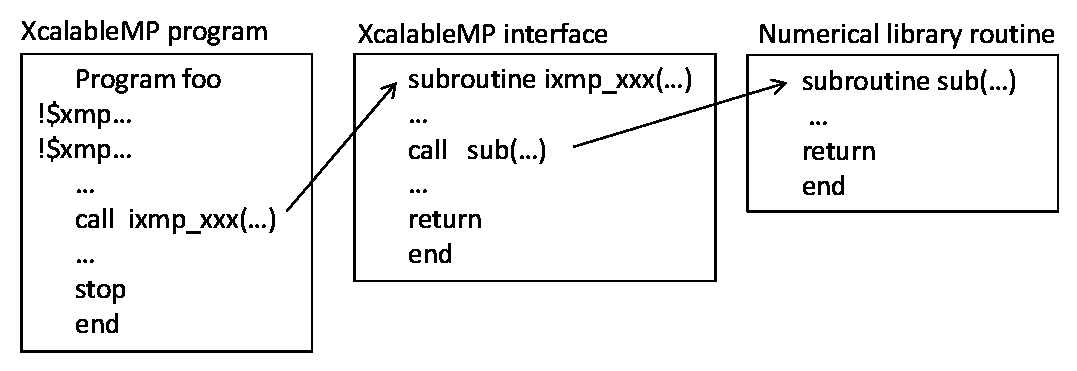
\includegraphics[scale=0.45]{figs/figb.1.eps}
  \caption{Invocation of a Library Routine through an Interface Procedure}
  \label{figb.1}
 \end{myfigure}

 \item When the numerical library routine needs information on an global
       array, the interface extracts it from the descriptor using some
       query routines provided by {\XMP} and passes it to the
       numerical library routine as arguments.
%
 \item The interface does not affect the behavior of numerical library
       routines except for restrictions concerning the {\XMP}
       specification.
\end{itemize}


\section{Query routines}

Specifications of some query routines are shown below.

\subsection{\tt xmp\_node\_index}
\index{xmp\_node\_index@{\tt xmp\_node\_index}}

\subsubsection*{Format}

\begin{tabular}{lll}

\verb![F]!& {\tt subroutine}& {\tt xmp\_node\_index(d, idx)}\\
          & {\tt integer(kind=xmp\_desc\_kind)} & {\tt d}\\
          & {\tt integer} & {\tt idx(dim)}\\

\verb![C]!&  {\tt void}& {\tt xmp\_node\_index(xmp\_desc\_t d, int idx[])}\\

\end{tabular}

\subsubsection*{Synopsis}

The {\tt xmp\_node\_index} routine provides the indices of the
executing node in the target node array.

\subsubsection*{Arguments}

\begin{itemize}
 \item {\tt d} is a descriptor, that is, an object of type {\tt
       integer(kind=xmp\_desc\_kind)}, in {\XMP}, or {\tt xmp\_desc\_t},
       in {\XMPC}, that is associated with the node array.
 \item {\tt idx} is a one-dimensional integer array. {\tt
       dim} is the rank of the node array.
\end{itemize}


\subsection{\tt xmp\_node\_size}
\index{xmp\_node\_size@{\tt xmp\_node\_size}}

\subsubsection*{Format}

\begin{tabular}{lll}

\verb![F]!& {\tt subroutine}& {\tt xmp\_node\_size(d, size)}\\
          & {\tt integer(kind=xmp\_desc\_kind)} & {\tt d}\\
          & {\tt integer} & {\tt size(dim)}\\

\verb![C]!&  {\tt void}& {\tt xmp\_node\_size(xmp\_desc\_t d, int size[])}\\

\end{tabular}

\subsubsection*{Synopsis}

The {\tt xmp\_node\_size} routine provides the size of each dimension of
the target node array.

\subsubsection*{Arguments}

\begin{itemize}
 \item {\tt d} is a descriptor, that is, an object of type {\tt
       integer(kind=xmp\_desc\_kind)}, in {\XMP}, or {\tt xmp\_desc\_t},
       in {\XMPC}, that is associated with the node array.
 \item {\tt size} is a one-dimensional integer array. {\tt
       dim} is the rank of the node array.
\end{itemize}

\subsection{\tt xmp\_gt\_size}
\index{xmp\_gt\_size@{\tt xmp\_gt\_size}}

\subsubsection*{Format}

\begin{tabular}{lll}

\verb![F]!& {\tt subroutine}& {\tt xmp\_gt\_size(d, size)}\\
          & {\tt integer(kind=xmp\_desc\_kind)} & {\tt d}\\
          & {\tt integer} & {\tt size(dim)}\\

\verb![C]!&  {\tt void}& {\tt xmp\_gt\_size(xmp\_desc\_t d, int size[])}\\

\end{tabular}

\subsubsection*{Synopsis}

The {\tt xmp\_gt\_size} routine provides the global size of each
dimension of the target template.

\subsubsection*{Arguments}

\begin{itemize}
 \item {\tt d} is a descriptor, that is, an object of type {\tt
       integer(kind=xmp\_desc\_kind)}, in {\XMP}, or {\tt xmp\_desc\_t},
       in {\XMPC}, that is associated with the target template.
 \item {\tt size} is a one-dimensional integer array. {\tt
       dim} is the rank of the template.
\end{itemize}

\subsection{\tt xmp\_lt\_size}
\index{xmp\_lt\_size@{\tt xmp\_lt\_size}}

\subsubsection*{Format}

\begin{tabular}{lll}

\verb![F]!& {\tt subroutine}& {\tt xmp\_lt\_size(d, size)}\\
          & {\tt integer(kind=xmp\_desc\_kind)} & {\tt d}\\
          & {\tt integer} & {\tt size(dim)}\\

\verb![C]!&  {\tt void}& {\tt xmp\_lt\_size(xmp\_desc\_t d, int size[])}\\

\end{tabular}

\subsubsection*{Synopsis}

The {\tt xmp\_lt\_size} routine provides the local size of each dimension
of the target template.

\subsubsection*{Arguments}

\begin{itemize}
 \item {\tt d} is a descriptor, that is, an object of type {\tt
       integer(kind=xmp\_desc\_kind)}, in {\XMP}, or {\tt xmp\_desc\_t},
       in {\XMPC}, that is associated with the template.
 \item {\tt size} is a one-dimensional integer array. {\tt
       dim} is the rank of the template.
\end{itemize}


\subsection{\tt xmp\_ga\_size}
\index{xmp\_ga\_size@{\tt xmp\_ga\_size}}

\subsubsection*{Format}

\begin{tabular}{lll}

\verb![F]!& {\tt subroutine}& {\tt xmp\_ga\_size(d, size)}\\
          & {\tt integer(kind=xmp\_desc\_kind)} & {\tt d}\\
          & {\tt integer} & {\tt size(dim)}\\

\verb![C]!&  {\tt void}& {\tt xmp\_ga\_size(xmp\_desc\_t d, int size[])}\\

\end{tabular}

\subsubsection*{Synopsis}

The {\tt xmp\_ga\_size} routine provides the global size of each
dimension of the target global array.

\subsubsection*{Arguments}

\begin{itemize}
 \item {\tt d} is a descriptor, that is, an object of type {\tt
       integer(kind=xmp\_desc\_kind)}, in {\XMP}, or {\tt xmp\_desc\_t},
       in {\XMPC}, that is associated with the global array.
 \item {\tt size} is to be set to a one-dimensional integer array. {\tt
       dim} is the rank of the global array.
\end{itemize}

\subsection{\tt xmp\_la\_size}
\index{xmp\_la\_size@{\tt xmp\_la\_size}}

\subsubsection*{Format}

\begin{tabular}{lll}

\verb![F]!& {\tt subroutine}& {\tt xmp\_la\_size(d, size)}\\
          & {\tt integer(kind=xmp\_desc\_kind)} & {\tt d}\\
          & {\tt integer} & {\tt size(dim)}\\

\verb![C]!&  {\tt void}& {\tt xmp\_la\_size(xmp\_desc\_t d, int size[])}\\

\end{tabular}

\subsubsection*{Synopsis}

The {\tt xmp\_la\_size} routine provides the local size of each
dimension of the global array.

\subsubsection*{Arguments}

\begin{itemize}
 \item {\tt d} is a descriptor, that is, an object of type {\tt
       integer(kind=xmp\_desc\_kind)}, in {\XMP}, or {\tt xmp\_desc\_t},
       in {\XMPC}, that is associated with the global array.
 \item {\tt size} is a one-dimensional integer array. {\tt
       dim} is the rank of the global array.
\end{itemize}

\subsection{\tt xmp\_ga\_template\_unitsize}
\index{xmp\_ga\_template\_unitsize@{\tt xmp\_ga\_template\_unitsize}}

\subsubsection*{Format}

\begin{tabular}{lll}

\verb![F]!&  {\tt subroutine}& {\tt xmp\_ga\_template\_unitsize(d, unitsize)}\\
          & {\tt integer(kind=xmp\_desc\_kind)} & {\tt d}\\
          & {\tt integer} & {\tt unitsize(dim)}\\

\verb![C]!&  {\tt void}& {\tt xmp\_ga\_template\_unitsize(xmp\_desc\_t d, int unitsize[])}\\

\end{tabular}

\subsubsection*{Synopsis}

The {\tt xmp\_ga\_template\_unitsize} routine provides the blocking
factor of each dimension of the target template.

\subsubsection*{Arguments}

\begin{itemize}
 \item {\tt d} is a descriptor, that is, an object of type {\tt
       integer(kind=xmp\_desc\_kind)}, in {\XMP}, or {\tt xmp\_desc\_t},
       in {\XMPC}, that is associated with the template.
 \item {\tt unitsize} is a one-dimensional integer array. {\tt dim} is
       the rank of the template.
\end{itemize}


\subsection{\tt xmp\_ga\_first\_idx\_node\_index}
\index{xmp\_ga\_first\_idx\_node\_index@{\tt
xmp\_ga\_first\_idx\_node\_index}}

\subsubsection*{Format}

\begin{tabular}{lll}

\verb![F]!&  {\tt subroutine}& {\tt xmp\_ga\_first\_idx\_node\_index(d, idx)}\\
          & {\tt integer(kind=xmp\_desc\_kind)} & {\tt d}\\
          & {\tt integer} & {\tt idx(dim)}\\

\verb![C]!&  {\tt void}& {\tt xmp\_ga\_first\_idx\_node\_index(xmp\_desc\_t d, int idx[])}\\

\end{tabular}

\subsubsection*{Synopsis}

The {\tt xmp\_ga\_first\_idx\_node\_index} routine provides the indices
of the node onto which the {\it first} element of the global array is
distributed.

\subsubsection*{Arguments}

\begin{itemize}
 \item {\tt d} is a descriptor, that is, an object of type {\tt
       integer(kind=xmp\_desc\_kind)}, in {\XMP}, or {\tt xmp\_desc\_t},
       in {\XMPC}, that is associated with the global array.
 \item {\tt idx} is a one-dimensional integer array. {\tt dim} is the
       rank of node array associated with the global array.
\end{itemize}


\subsection{\tt xmp\_la\_lead\_dim}
\index{xmp\_la\_lead\_dim@{\tt xmp\_la\_lead\_dim}}

\subsubsection*{Format}

\begin{tabular}{lll}

\verb![F]!&  {\tt subroutine}& {\tt xmp\_la\_lead\_dim(d, lead\_dim)}\\
          & {\tt integer(kind=xmp\_desc\_kind)} & {\tt d}\\
          & {\tt integer} & {\tt lead\_dim}\\

\verb![C]!&  {\tt void}& {\tt xmp\_la\_lead\_dim(xmp\_desc\_t d, int lead\_dim)}\\

\end{tabular}

\subsubsection*{Synopsis}

The {\tt xmp\_la\_lead\_dim} routine provides the leading dimension of
each local section of the target global array.

\subsubsection*{Arguments}

\begin{itemize}
 \item {\tt d} is a descriptor, that is, an object of type {\tt
       integer(kind=xmp\_desc\_kind)}, in {\XMP}, or {\tt xmp\_desc\_t},
       in {\XMPC}, that is associated with the global array.
 \item {\tt lead\_dim} is an integer scalar.
\end{itemize}


%\subsection{\tt xmp\_la\_addr}
%
%\subsubsection*{Format}
%
%\begin{tabular}{lll}
%
%\verb![F]!&  {\tt subroutine}& {\tt xmp\_la\_addr(d, addr)}\\
%          & {\tt xmp\_desc\_t} & {\tt d}\\
%          & {\tt integer, allocatable} & {\tt addr}\\
%
%\verb![C]!&  {\tt void}& {\tt xmp\_la\_addr(xmp\_desc\_t d, int* addr)}\\
%
%\end{tabular}
%
%\subsubsection*{Synopsis}
%
%The {\tt xmp\_la\_addr} routine provides the base address of each local
%section of the target global array.
%
%\subsubsection*{Arguments}
%
%\begin{itemize}
% \item {\tt d} is a descriptor, that is, an object of type {\tt
%       xmp\_desc\_t} that is associated with the global array.
% \item {\tt addr} is the base address of the local array.
%\end{itemize}


\section{Example}
\index{Example!library interface}

   This section shows the interface to ScaLAPACK as an example of the
   {\XMP} interface to numerical libraries.
   
   ScaLAPACK is a linear algebra library for distributed-memory.
   Communication processes in the ScaLAPACK routines depends on BLACS
   (Basic Linear Algebraic Communication Subprograms).
   ScaLAPACK library routines invoked from {\XMP} procedures also depend
   on BLACS. %Remarks of the design of the interface are as follows.

%\begin{itemize}
%\item For a ScaLAPACK library routine having a descriptor array as an
%      argument, the interface procedure has the BLACS context handle
%      including the descriptor array as an additional argument.
%\item The {\tt blacs\_exit} routine is unnecessary because an {\XMP}
%      program executes {\tt MPI\_Finalize}.
%\item Only ``column-major'' is effective as the argument ``order'' of a
%      BLACS routine {\tt blacs\_gridinit}.
%\end{itemize}

\begin{description}

 \item[Example 1]
	    This example shows an implementation of the interface for
	    the ScaLAPACK driver routine {\tt pdgesv}.

\begin{XFexample}
      subroutine ixmp_pdgesv(n,nrhs,a,ia,ja,da,ipiv,b,ib,jb,db,ictxt,info)

      use xmp_lib

      integer n,nrhs,ia,ja,ib,jb,ictxt,info
      double precision a,b
      integer(kind=xmp_desc_kind) da,db
      integer size_a(2),unitsize_a(2),rank_a(2),lead_dim_a,desca(9)
      integer size_b(2),unitsize_b(2),rank_b(2),lead_dim_b,descb(9)
      
      call xmp_ga_size(da,size_a)
      call xmp_ga_template_unitsize(da,unitsize_a)
      call xmp_ga_first_idx_nodes_rank(da,rank_a)
      call xmp_la_lead_dim(da,lead_dim_a)
      
      call xmp_ga_size(db,size_b)
      call xmp_ga_template_unitsize(db,unitsize_b)
      call xmp_ga_first_idx_nodes_rank(db,rank_b)
      call xmp_la_lead_dim(db,lead_dim_b)
      
      desca(1)=1
      desca(2)=ictxt
      desca(3)=size_a(1)
      desca(4)=size_a(2)
      desca(5)=unitsize_a(1)
      desca(6)=unitsize_b(2)
      desca(7)=rank_a(1)
      desca(8)=rank_a(2)
      desca(9)=lead_dim_a
      
      descb(1)=1
      descb(2)=ictxt
      descb(3)=size_b(1)
      descb(4)=size_b(2)
      descb(5)=unitsize_b(1)
      descb(6)=unitsize_b(2)
      descb(7)=rank_b(1)
      descb(8)=rank_b(2)
      descb(9)=lead_dim_b
      
      call pdgesv(n,nhrs,a,ia,ja,desca,ipiv,b,ib,jb,descb,info)
      
      return
      end

\end{XFexample}


\item[Example 2]
	   This example shows an {\XMP} procedure using the interface of
	   Example 1.

\Example{nodes}
\Example{template}
\Example{distribute}
\Example{align}
\Example{loop}
\begin{XFexample}
      program xmptdgesv

      use xmp_lib

      double precision a(1000,1000)
      double precision b(1000)
      integer ipiv(2*1000,2)
!$xmp nodes p(2,2)
!$xmp template t(1000,1000)
!$xmp template t1(2*1000,2)
!$xmp distribute t(block,block) onto p
!$xmp distribute t1(block,block) onto p
!$xmp align a(i,j) with t(i,j)
!$xmp align ipiv(i,j) with t1(i,j)
!$xmp align b(i) with t(i,*)
      ...
      integer i,j,ictxt
      integer m=1000,n=1000,nprow=2,npcol=2
      integer icontxt=-1,iwhat=0
      integer nrhs=1,ia=1,ja=1,ib=1,jb=1,info
      character*1 order
      ...
      order="C"
      ...
      call blacs_get(icontxt,iwhat,ictxt)
      call blacs_gridinit(ictxt,order,nprow,npcol)
      ...
!$xmp loop (i,j) on t(i,j)
      do j=1,n
         do i=1,m
            a(i,j) = ...
         end do
      end do
      ...
!$xmp loop on t(i,*)
      do i=1,m
         b(i)= ...
      end do
      ...
      call ixmp_pdgesv(n,nrhs,a,ia,ja,xmp_desc_of(a),ipiv,
     *                b,ib,jb,xmp_desc_of(b),ictxt,info)
      ...
      call blacs_gridexit(ictxt)
      ...
      stop
      end
\end{XFexample}
\end{description}

\cleardoublepage


 \chapter{XcalableMP I/O(Proposal)}

 \section{Categorization of I/O}
 XcalableMP has three kinds of I/O.

  \subsection{Local I/O}

  Local I/O is the way to use I/O statements and I/O service functions in
  base languages, in which I/O statements and functions are used without
  any directives.

  I/O statements (in {\XMP} {\Fort}) and I/O functions (in {\XMP} {\C})
  are executed in local similar to the other execution statements.
  It depends on the system which nodes can handle the I/O statements and
  functions.

  Local I/O can read a file written by the base language and, vice
  versa.

  [F] A name of a global array in the I/O list describes the
  entire area of the array located in each node.

  An array element of a global array can be referred as an I/O item only
  in the node where it is located.

  [F] Any array section of a global array cannot be referred as an
  I/O item.

  \subsection{Master I/O[F]}

  Master I/O is input and output for the file that corresponds to an
  execution node set.
  Master I/O is global execution.

  In master I/O, a global data is input and output as if it is executed
  only by master node, which represents the execution node set, through
  its local copy of the data.

  Master node is chosen among the execution node set arbitrarily by the
  system, and is unique to the execution node set during execution of
  the program.

  Master I/O is provided in the form of directives of {\XMP} {\Fort}.

  A global array as an I/O item is accessed in the sequential order of
  array elements.
  When a local variable is read from a file, the value is copied to all
  nodes of the execution node set.
  When a local variable or an expression is written to a file, only the
  value of the data on master node is written.
  
  Master I/O can read a file written by the base language, and vice
  versa.
  

  \subsection{Global I/O}

  Also global I/O is input and output for the file that corresponds to
  an execution node set.
  Some executions of global I/O are global and the others are local.
  In a large system with many nodes, global I/O can be expected higher
  speed and less memory consumption execution than master I/O.

  [F] It is provided in the form of directives for a part of I/O
  statements, such as OPEN, CLOSE, READ
  and WRITE statements.

  [C] It is provided in the form of service functions and include files.

  Global I/O can handle only unformatted (binary) files. In XcalableMP Fortran,
  implied DO-Loops and some specifiers cannot be used.
  In XcalableMP C, a formatted I/O library, including fprintf() and fscanf(), is not provided.

  Global I/O can read a file written in MPI-IO, and vice versa. 

  [F] File formats are not compatible between XcalableMP Fortran
  and the base language because global I/O does not generate or access
  the file header and footer particular to the base language.

  There are three kinds of Global I/O, as shown in Table
  \ref{tb:global}.
  {\bf Collective} global I/O is global (collective) execution and
  sequential file access.
  It handles global data in the sequential order, similar to master
  I/O.
  {\bf Atomic} global I/O is local execution and sequential file access.
  Execution nodes share file positioning of the global I/O file and
  execute each I/O statement and library call mutually.
  {\bf Direct} global I/O is local execution and direct file access.
  Each execution node has its own file positioning and accesses a shared
  file concurrently.

  \begin{table}[tb]
   \begin{center}
    \caption{Global I/O}
    \label{tb:global}
    \begin{tabular}{|c||l|l|}
     \hline 
     & independent/collective & access method  \\ \hline \hline
     Collectibe I/O & collective & sequential access \\ \hline
     Atomic I/O & independent & sequential access \\ \hline
     Direct I/O & independent & direct access \\ \hline
    \end{tabular}
   \end{center}
  \end{table}
  
  Restriction

  \begin{itemize}
   \item  The name of a global array may not be declared in a namelist
	  group.
	  That is, NAMELIST I/O is not allowed for global arrays.
  \end{itemize}

  Advice for programmers

  Local I/O is useful for debugging focusing on a node since local I/O
  is executed on each node individually.

  Master I/O is a directive extension, in which the execution result
  matches the one of the base language ignoring directive lines.

  Global I/O aims for highly-parallel I/O using thousands of nodes.
  It is limited to binary file.
  It avoids extreme concentration of computational load and memory
  consumption to specific nodes using MPI-IO or other parallel I/O
  techniques.

  \section{File Connection}

  A file is connected to a unit in XcalableMP Fortran and to a file
  handler in XcalableMP C.
  This operation is called {\bf file connection}.
  Local I/O connects a file in each node independently.
  Master I/O and global I/O connect a file to an execution node set
  collectively.
  
  There are two ways of file connections, dynamic connection and
  preconnection.
  Dynamic connection connects a file during execution of the program.
  Preconnection connects a file at the begininng of execution of the
  program and therefore it can execute I/O statements and functions
  without the prior execution of an OPEN statement or a function call to
  open the file.

  \subsection{File connection in local I/O}

  The language processor of the base language connects the file in each
  node.
  File system visible to each node is implementation dependent.

  It is implementation dependent which nodes can access the standard
  input, output and error files.
  It is also implementation dependent how behave the nodes accessing the
  same file at the same time; e.g., data in the standard input file may
  be read only one node and may be replicated all nodes.
  It is implementation dependent how data from the multiple nodes are
  merged into the standard output/error file.
  
  \subsection{File connection in master I/O [F]}

  An OPEN statement specified with a master I/O directive connects the
  master I/O file to the execution node set.
  When a master I/O file is connected by a READ statement or a WRITE
  statement without encountering any OPEN statement, the name and
  attribute of the file depend on the language system of the base
  language.
  Disconnection from a master I/O file is executed by a CLOSE statement
  or termination of the program.

  Dynamic connection must be executed concurrently by all nodes sharing
  the file with the same unit number.
  Two execution node sets may employ the same unit number only if they
  have no common node.

  The standard input, output and error files are preconnected to the
  entire node set.
  Therefore, master I/O executed on the entire node set is always
  allowed without OPEN and CLOSE statements.


  \subsection{File connection in global I/O}

  Dynamic connecton of global I/O is global (collective) execution and
  is valid for the execution node set.
  Global I/O file cannot be preconnected.

  \subsubsection*{[F]}

  An OPEN statement specified with a global I/O directive connects the
  global I/O file to the execution node set.
  Disconnection from a global I/O file is executed by a CLOSE statement
  or termination of the program.

  Dynamic connection must be executed concurrently by all nodes sharing
  the file with the same unit number.
  Two execution node sets may employ the same unit number only if they
  have no common node.

  \subsubsection*{[C]}

  A library function to open a global I/O file connect the file to the
  execution node set.
  Disconnection from a global I/O file is executed by a library function
  to close the file or termination of the program.

  \section{Master I/O}

  \subsection*{Summary}
  A master I/O construct executes data transfer between a file and an
  execution node set via master node of the execution node set.
  For a global array, the virtual sequential order of the array elements
  is visible.

  \subsection*{Syntax}
%  \Syntax{tasks}

  \begin{tabular}{ll}
   \verb![F]! & \verb|!$xmp| {\tt \verb|master_io|} \\
   & \hspace{5mm} {\it io-statement} \\
   & \\
   \verb![F]! & \verb|!$xmp| {\tt \verb|master_io|} begin \\
   & \hspace{5mm}{\it io-statement} \\
   & \hspace{5mm}... \\
   & \verb|!$xmp| {\tt \verb|master_io|} end \\
  \end{tabular}

   where {\it io-statement} is one of:

   \begin{itemize}
    \item OPEN statement
    \item CLOSE statement
    \item READ statement
    \item WRITE statement
    \item PRINT statement
    \item BACKSPACE statement
    \item ENDFILE statement
    \item REWIND statement
    \item INQUIRE statement
   \end{itemize}

   \subsection*{Restriction}
   \begin{itemize}
    \item The following items cannot be specified in the input item list.

	  \begin{itemize}
	   \item Array section of global array
	   \item Substring of global array
	   \item Array element whose subscript contains reference of a
		 global array
	   \item Array section whose subscript contains reference of a
		 global array
	   \item Substring whose subscript contains reference of a
		 global array
	   \item Expressions including the global array reference
	   \item I/O implied DO
	  \end{itemize}

    \item An I/O statement specified with a master I/O directive must be
	  executed on the node set that is connected to the file.
    \item Internal file I/O is not allowed as a master I/O.
   \end{itemize}
	  
  \subsection*{Description}

   An I/O statement specified with a master I/O directive accesses to a
   file whose format is the same as the one of the base language.
   The access, including connection, disconnection, input and output,
   file positioning, and inquiry, is global (collective) and must be
   executed on the same node set as the one where the file was
   connected. 

   Master node, a unique node to a execution node set, is chosen by the
   language system.
   Master I/O works as if all file access is executed only on the master
   node.

   The operations for I/O items are summarized in the following table.

   \begin{table}[h]
    \begin{center}
     \begin{tabular}{|l|p{40mm}|p{80mm}|}
      \hline
      \multicolumn{1}{|c}{ }  & {\bf I/O item} & {\bf operation} \\
      \hline
      input item & name of global array & The data that is read 
	      from the file in the sequential order of array elements is distributed onto 
	      the global array on the node set. The file positioning increases by
	      the size of data. \\
      \cline{2-3}
      & array element of global array &  The data that is read from the file
	      is copied to the element of the global array on the specific node.
	      The file positioning increases by the size of data. \\
      \cline{2-3}
      & local variable & The data that is read from the file is replicated to the
	      local variables on all nodes of the execution node
	      set. The file positioning increases by the size of data. \\
      \cline{2-3}
      & inplied DO-loop & For each input item, repeats the above operation. \\
      \hline
      output item & name of global array & The value of the
	      global array is collected and is written to the
	      file in the sequential order of array elements. The file
	      positioning increases by the size of data. \\
      \cline{2-3}
      & array element of global array &  The value of the element of the
	      global array is written to the
	      file. A file position increases by data length. \\
      \cline{2-3}
      & local variable and expression & The value evaluated on the master node
	      is written to the file. The file positioning increases by
	      the size of data. \\
      \cline{2-3}
      & inplied DO-loop & For each output item, repeat the above operation. \\
      \hline
      \end{tabular}
     \end{center}
%    \caption{aaa}
    \label{tb:aaa}
   \end{table}

   Namelist input and output statements cannot treat global arrays.
   A namelist output statement writes the value on the master node to
   the file.
   In the namelist input, each item of the namelist is read from the
   file to the master node if it is recorded in the file.
   And then all items of the namelist are replicated onto all nodes of
   the execution node set even if any item is not read from the file.

   IOSTAT and SIZE specifiers and specifiers of the INQUIRE statement
   that can return values always return the same value among the
   execution node set.

   When a condition specified with ERR, END or EOR specifier is
   satisfied, all nodes of execution node set are branched together to
   the same statement.

   Advice to the implementer

   It is recommended to provide such a compiler option that local I/O
   statements (specified without directives) is regarded as master I/O
   statements (specified with master\_io directives).

   \clearpage
   
   \section{Global I/O}

   Global I/O executes data transfer between a file and global arrays
   distributed on the execution node set.
   Global I/O is restricted within unformatted (binary) files, but
   higher performance and lower memory consumption can be expected than
   master I/O.
   The file format is compatible with the one in MPI-IO.

   Global I/O consists of three kinds, collective I/O, atomic I/O, and
   direct I/O. 

   \subsection{Global I/O construct [F]}
   \subsubsection*{Syntax}

   \begin{tabular}{ll}
   \verb![F]! & \verb|!$xmp| {\tt \verb|global_io|} [atomic / direct] \\
   & \hspace{5mm} {\it io-statement} \\
   & \\
   \verb![F]! & \verb|!$xmp| {\tt \verb|global_io|} [atomic / direct] begin \\
   & \hspace{5mm}{\it io-statement} \\
   & \hspace{5mm}... \\
   & \verb|!$xmp| {\tt \verb|global_io|} end \\
   \end{tabular}

   The first syntax is just a shorthand of the second syntax.

   \subsubsection*{Restriction}

   I/O statements and specifiers available for {\it io-statement} is
   shown in the following table.
   Definition of each specifier is described in the specification of the base language. 

   Case of global\_io construct without direct clause:
   \begin{table}[h]
   \begin{center}
    \label{tb:globalstatement}
    \begin{tabular}{|c||l|}
      \hline
     I/O statement & available specifiers \\ \hline \hline
     OPEN & UNIT, IOSTAT, FILE, STATUS, POSITION, ACTION \\ \hline
     CLOSE & UNIT, IOSTAT, STATUS \\ \hline
     READ & UNIT, IOSTAT \\ \hline
     WRITE & UNIT, IOSTAT \\ \hline
    \end{tabular}
   \end{center}
   \end{table}

   Case of global\_io construct with direct clause:
   \begin{table}[h]
   \begin{center}
    \label{tb:globalstatement}
    \begin{tabular}{|c||l|}
      \hline
     I/O statement & available specifiers \\ \hline \hline
     OPEN & UNIT, IOSTAT, FILE, STATUS, RECL, ACTION \\ \hline
     CLOSE & UNIT, IOSTAT, STATUS \\ \hline
     READ & UNIT, REC, IOSTAT \\ \hline
     WRITE & UNIT, REC, IOSTAT \\ \hline
    \end{tabular}
   \end{center}
   \end{table}

   Only the name of a variable (including global variable) can be specified 
   as the input item of READ statement specified with global\_io directive,
   but array element, array section,
   structure component, substring, and implied-DO loop are not allowed as input items.

   Only the name of a global array and an
   expression excluding global array reference can be specified as the output item
   of WRITE statement specified with global\_io directive, 
   but an expression including global array
   reference and implied-DO loop are not allowed as input items.


   \subsubsection*{Description}

   Global I/O construct connects, disconnects, inputs and outputs the global I/O file,
   which is compatible with MPI-IO.

   The standard input, output and error files cannot be a Global I/O file.
   A Global I/O file cannot preconnect to any unit or any file handler,
   and must explicitly be connected by the OPEN statement specified with
   global\_io directive.

   The OPEN statement specified with global\_io directive is global
   (collective) execution, and the file is shared in the execution node
   set.
   A file that is already open by the other OPEN statement with
   global\_io directive cannot be reopen by an OPEN statement with or
   without global\_io directive.

   A global I/O file must be disconnected explicitly by a CLOSE
   statement specified with global\_io directive, else the result of I/O
   is not guaranteed.
   The CLOSE statement specified with global\_io directive is a global
   (collective) execution and must be executed by the same execution
   node set as the one where the OPEN statement is executed.

   Available values of the specifiers in I/O statements are shown in the
   following table.
   Definitions of the specifiers are described in the specification of
   the base language.

   \begin{itemize}
    \item OPEN statement
   
   \begin{table}[h]
    \begin{center}
     \label{tb:globalopen}
     \begin{tabular}{|c||p{90mm}|l|}
       \hline
      specifiers & value & default \\ \hline \hline
      UNIT & external file unit (scalar constant expression)
	  & not omissible. \\ \hline
      FILE & file name (scalar CHARACTER expression)
	  & not omittable. \\ \hline
      STATUS & 'OLD', 'NEW', 'REPLACE' or 'UNKNOWN' & 'UNKNOWN' \\ \hline
      POSITION\footnote{available only if the directive has no directive
      clause} & 'ASIS', 'REWIND' or 'APPEND' & 'ASIS' \\ \hline
      ACTION & 'READ', 'WRITE' or 'READWRITE' & 'READWRITE' \\ \hline
      RECL\footnote{available only if the directive has a directive clause} & the value of the record length (scalar constant expression)
	  & not omittable. \\ \hline
     \end{tabular}
    \end{center}
   \end{table}

    \item CLOSE statement
	  
   \begin{table}[h]
    \begin{center}
     \label{tb:globalopen}
     \begin{tabular}{|c||p{90mm}|l|}
        \hline
      specifiers & value & default \\ \hline \hline
      UNIT & external file unit (scalar constant expression)
	  & omittable. \\ \hline
      STATUS & 'KEEP' or 'DELETE'
	  & 'KEEP' \\ \hline
     \end{tabular}
    \end{center}
   \end{table}

    \item READ/WRITE statement
	  
   \begin{table}[h]
    \begin{center}
     \label{tb:globalopen}
     \begin{tabular}{|c||p{90mm}|l|}
       \hline
      specifiers & value & default \\ \hline \hline
      UNIT & external file unit (scalar constant expression)
	  & not omittable. \\ \hline
      REC\footnote{available only if the directive has a directive clause} & the value of the record length (scalar constant expression)
	  & not omittable. \\ \hline
     \end{tabular}
    \end{center}
   \end{table}

    \item When a scalar default INTEGER variable is set to IOSTAT, an
	  error code is set to the specifiers.
	 
   \end{itemize}

   OPEN, CLOSE, READ and WRITE statements specified with global\_io directives
   without atomic and direct clauses are called respectively collective OPEN, collective
   CLOSE, collective READ, and collective WRITE statements respectively.
   These all statements are called collective I/O statements.

   OPEN, CLOSE, READ and WRITE statements specified with global\_io directives
   with atomic clauses are called atomic OPEN, atomic CLOSE, atomic READ, and
   atomic WRITE statements respectively.
   These all statements are called atomic I/O statements.

   OPEN, CLOSE, READ and WRITE statements specified with global\_io directives
   with direct clause are called direct OPEN, direct CLOSE, direct READ, and
   direct WRITE statements respectively.
   These all statements are called direct I/O statements.

   The file connected by collective, atomic or direct OPEN statement can
   be read/be written only by the same type of READ/WRITE statement.
   The file can be disconnected by the same type of CLOSE statement.
   Different types of global I/O cannot be executed together for the same file or the
   same unit.
   For example, atomic I/O statements cannot be executed for the unit
   connected by a collective OPEN statement.

   \clearpage
   
   \subsubsection{collective I/O statement}

   Collective I/O statements read/write for a file shared between nodes.
   I/O data remains the image of global array.

   Collective I/O statements are matched across all nodes.
   In collective I/O, I/O operations, such as connection, disconnection,
   read and write, for a file must be executed in the same nodes. 
   
   The operations for I/O items are summarized in the following table.

   \begin{table}[h]
    \begin{center}
     \begin{tabular}{|l|r|p{80mm}|}
      \hline
      \multicolumn{1}{|c}{ }  & {\bf I/O item} & {\bf operation} \\ \hline
      input item & name of distributed array & The value is read along
	      the file view set in a template. The value is set to array
	      elements in each node.
	      File position seeks by data size.\\
      \cline{2-3}
      & duplicate variable &  The value set from a file is set in a
	      duplicate array in all nodes. File position seeks by
	      data length. \\ \hline
      output item & name of distributed array & The value is written
	      along the file view set in a template. The value is
	      written for a file.
	      File position seeks by data size.\\
      \cline{2-3}
      & duplicate variable, expression & The value in any one node is
	      written to the file.  File position seeks by data
	      length. \\ \hline
      \end{tabular}
     \end{center}
%    \caption{aaa}
    \label{tb:aaa}
   \end{table}

   \subsubsection{atomic I/O statement}

   Atomic I/O statements exclusively read/write for a file shared
   between nodes in no particular order.
   As nondeterministic parallel execution, if the program is the same,
   the results can differ.

   Atomic OPEN and CLOSE statements are executed collectively. Atomic
   READ and WRITE statements are executed locally.
   The file connected by atomic OPEN statements is disconnected by using
   atomic CLOSE statements in all execution nodes.
   Atomic READ and WRITE statements can be executed from any node in a
   set of execution nodes.

   Atomic READ and WRITE statements are exclusively excuted.
   A unit of atomic I/O statements is a READ statement or a WRITE
   statement.

   At first, the file position is determined by the POSITION specifier in
   atomic I/O statement.
   After that, file position seeks by the length of the input/output
   variables.


   \subsubsection{direct I/O statement}

   Direct I/O statements read/write for a file shared between nodes.
   File position is specified on each node.

   Direct OPEN and CLOSE statements are executed collectively. Direct
   READ and WRITE statements are executed locally.
   The file connected by direct OPEN statements is disconnected by using
   atomic CLOSE statements in all execution nodes.
   Direct READ and WRITE statements can be executed from any node in a
   set of execution nodes.
   
   Direct READ and WRITE statements read/write to file position
   specified by a REC specifier.
   Direct READ and WRITE statements are executed independently.
   File position is the value multiplied by the value specified in a RECL
   specifiers and the value specified in a REC specifier.


   \subsection{Global I/O library [C]}

   In C, some of data types is defined in an include file.
   A set of library functions with the arguments of the data type is
   provided.
   Built-in function gotten these type from the name of a distributed
   array is provided.
   The following types are provided.

   \begin{itemize}
    \item xmp\_file\_t : file handle
    \item xmp\_array\_t : distributed data for a distributed
	  array
    \item xmp\_rang\_t : expression of array section
   \end{itemize}

   The following library functions are provided.
   Collective function names end with \_all.

   \begin{itemize}
    \item global I/O file operation
    \begin{itemize}
     \item xmp\_fopen\_all
     \item xmp\_fclose\_all
     \item xmp\_fseek
     \item xmp\_fseek\_shared\_all
     \item xmp\_ftell
     \item xmp\_ftell\_shared
     \item xmp\_file\_sync\_all
    \end{itemize}
    \item collective I/O
    \begin{itemize}
     \item xmp\_file\_set\_view\_all
     \item xmp\_file\_clear\_view\_all
     \item xmp\_fread\_all
     \item xmp\_fwrite\_all
     \item xmp\_fread\_darray\_all
     \item xmp\_fwrite\_darray\_all
    \end{itemize}
    \item atomic I/O
    \begin{itemize}
     \item xmp\_fread\_shared
     \item xmp\_fwrite\_shared
    \end{itemize}
    \item direct I/O
    \begin{itemize}
     \item xmp\_fread
     \item xmp\_fwrite
    \end{itemize}
   \end{itemize}

   \clearpage
   
   \subsubsection{Data type}

   The following data types are defined in include file ``xmp\_io.h''.
   \begin{description}
    \item[xmp\_file\_t] The valiable of xmp\_file\_t type is a file
	       handle.
	       The file handle is generated when a file is opened.
	       There are shared file pointer and intrinsic file pointer
	       to identify file position.

	       Shared file pointer share with shared nodes.
	       The file pointer is seeked by atomic I/O.
	       Identify file pointer is seeked by collective I/O and
	       direct I/O.
	       
	       These file pointers are managed by the member of
	       xmp\_file\_t type structures.
	       These file pointers are controled and referenced through
	       the library function.
	       
    \item[xmp\_array\_t] The valiable of xmp\_array\_t is distributed data
	       for a distributed array.
	       Distribution, alignment and node array shape, etc are the
	       member of xmp\_array\_t.

	       Distributed data of Distributed array ``A'' is gotten by
	       the following built-in function.
	       
	       xmp\_array\_t xmp\_array\_of(A);
	       
    \item[xmp\_range\_t] The valiable of xmp\_range\_t is an expression
	       of array section.
	       Lower bound, upper bound and stride are included in the
	       member of an array.
   \end{description}

   \subsubsection{Global I/O file operation}

   [OPEN]
   
   The function opens a global I/O file.
   \begin{table}[h]
    \begin{center}
      \begin{tabular}{|l|r|p{90mm}|}
      \hline
      {\bf function name}  & \multicolumn{2}{c|}{\bf xmp\_file\_t
      $*$xmp\_fopne\_all()}  \\ \hline
      argument & const char $*$fname & file name \\ \cline{2-3}
      & const char $*$amode & equialent to fopen of POSIX. combination
	      of ``rwa+'' \\ \hline
      return value & xmp\_file\_t$*$ & file structure. NULL is returned
	      when a program abend. \\ \hline
      \end{tabular}
     \end{center}
%    \caption{aaa}
    \label{tb:aaa}
   \end{table}

   File view is initialized. The value of shared file pointer and intrinsic file
   pointer depend on the value of amode.

   \begin{table}
     \begin{center}
    \label{tb:xxx}
    \begin{tabular}{|c|p{120mm}|}
      \hline
     amode & intended purpose \\ \hline \hline
     r &  Open for reading only. File pointer points the beginning of
	 the file.\\ \hline
     r+ & Open an existing file for update (reading and writing). File
	 pointer points the beginning of the file. \\ \hline
     w &  Create for writing. If a file by that name already exists, it
	 will be overwritten. File pointer points the begininng of th file. \\ \hline
     w+ & Create a new file for update (reading and writing). If a file
	 by that name already exists, it will be overwritten. File
	 pointer points the beginning of the file. \\ \hline
     a & Append; open for writing at end-of-file or create for writing
	 if the file does not eist. File pointer points the end of the file. \\ \hline
     a+ & Open for append; open (or create if the file does not exist)
	 for update at the end of the file. File pointer points the
	 beginning of the file. \\ \hline
    \end{tabular}
   \end{center}
   \end{table}


   \clearpage
   [CLOSE]

   The function closes a global I/O file.

   \begin{table}[h]
    \begin{center}
     \begin{tabular}{|l|l|p{80mm}|}
      \hline
      {\bf function name}  & \multicolumn{2}{c|}{\bf xmp\_file\_t
      $*$xmp\_fclose\_all(fh)} \\ \hline \hline
      argument & xmp\_file\_t $*$fh & file structure \\ \hline
      return value & int & 0: normal termination \\
      &  & 1: abnormal termination. fh is NULL. \\
      &  & 2: abnormal termination. error in MPI\_File\_close. \\ \hline
      \end{tabular}
     \end{center}
%    \caption{aaa}
    \label{tb:close}
   \end{table}

   [intrinsic file pointer setting]

   Change the setting of intrinsic file pointer.
   \begin{table}[h]
    \begin{center}
     \begin{tabular}{|l|r|p{70mm}|}
      \hline
      {\bf function name}  & \multicolumn{2}{c|}{\bf int xmp\_fseek(fh,
      offset, whence)}  \\ \hline \hline
      argument & xmp\_file\_t $*$fh & file structure \\ \cline{2-3}
      & long long offset & displacement of current file view from
	      position of whence \\ \cline{2-3}
      & int whence & choose file position \\
      &  & SEEK\_SET: the beginning of the file \\ 
      &  & SEEK\_CUR: current position \\ 
      &  & SEEK\_END: the end of the file \\ \hline
      return value & int & 0: normal termination \\
      &  & an integer othe than 0: abnormal termination \\ \hline
      \end{tabular}
     \end{center}
%    \caption{aaa}
    \label{tb:aaa}
   \end{table}

   \clearpage

   [shared file pointer setting]

   Change the setting of shared file pointer.
   \begin{table}[h]
    \begin{center}
     \begin{tabular}{|l|r|p{80mm}|}
      \hline
      {\bf function name}  & \multicolumn{2}{c|}{\bf int xmp\_fseek\_shared(fh,
      offset, whence)}  \\ \hline \hline
      argument & xmp\_file\_t $*$fh & file structure \\ \cline{2-3}
      & long long offset & displacement of current file view from
	      position of whence \\ \cline{2-3}
      & int whence & choose file position \\
      &  & SEEK\_SET: the beginning of the file \\ 
      &  & SEEK\_CUR: current position \\ 
      &  & SEEK\_END: the end of the file \\ \hline
      return value & int & 0: normal termination \\
      &  & an integer othe than 0: abnormal termination \\ \hline
      \end{tabular}
     \end{center}
%    \caption{aaa}
    \label{tb:aaa}
   \end{table}


   [referece to position of intrinsic file pointer]

   Refer to position of intrinsic file pointer.
   \begin{table}[h]
    \begin{center}
     \begin{tabular}{|l|r|p{80mm}|}
      \hline
      {\bf function name}  & \multicolumn{2}{c|}{\bf long long
      xmp\_ftell(fh)} \\ \hline \hline
      argument & xmp\_file\_t $*$fh & file structure \\ \hline
      return value & long long & Upon successful completion, the
	      function shall open the file and return a non-negative
	      integer representing the lowest numbered unused file
	      descriptor. Otherwise, negative number shall be
	      returned. \\ \hline
      \end{tabular}
     \end{center}
%    \caption{aaa}
    \label{tb:aaa}
   \end{table}
   

   
   [referece for position of shared file pointer]

   Refer to position of shared file pointer.
   \begin{table}[h]
    \begin{center}
     \begin{tabular}{|l|r|p{80mm}|}
      \hline
      {\bf function name}  & \multicolumn{2}{c|}{\bf long long
      xmp\_ftell\_shared(fh)} \\ \hline \hline
      argument & xmp\_file\_t $*$fh & file structure \\ \hline
      return value & long long & Upon successful completion, the
	      function shall open the file and return a non-negative
	      integer representing the lowest numbered unused file
	      descriptor. Otherwise, negative number shall be
	      returned. \\ \hline
      \end{tabular}
     \end{center}
%    \caption{aaa}
    \label{tb:aaa}
   \end{table}
   
   

   [file synchronization]

   File synchronizing.
   Completion of writing for a file from shared nodes is guaranteed.

   \begin{table}[h]
    \begin{center}
     \begin{tabular}{|l|r|p{80mm}|}
      \hline
      {\bf function name}  & \multicolumn{2}{c|}{\bf int
      xmp\_file\_sync\_all(fh)} \\ \hline \hline
      argument & xmp\_file\_t $*$fh & file structure \\ \hline
      return value & int & 0: normal termination \\
      &  & an integer othe than 0: abnormal termination \\ \hline
      \end{tabular}
     \end{center}
%    \caption{aaa}
    \label{tb:aaa}
   \end{table}

   \clearpage

   \subsubsection{collective I/O}

   Collective I/O is collectively executed.
   Collective I/O read/write from position of intrinsic file pointer.
   Assume that file view is previously set, where file view mechanism
   describes relationship between how nodes will access their data
   and how data laid out on disk.
   A detailed the definition of file view mechanism can be found in MPI
   2.0 specificaation.

   [file view setting]

   The function sets file view.

   \begin{table}[h]
    \begin{center}
     \begin{tabular}{|l|r|p{70mm}|}
      \hline
      {\bf function name}  & \multicolumn{2}{c|}{\bf int xmp\_file\_set\_view\_all(fh,
      disp, ap, rp)} \\ \hline \hline
      argument & xmp\_file\_t $*$fh & file structure \\ \cline{2-3}
      & long long disp & displacement from the beginning of the file. \\ \cline{2-3}
      & xmp\_array\_t ap & data of distributed array \\ \cline{2-3}
      & xmp\_range\_t $*$rp & data of accessible range \\ \hline
      return value & int & 0: normal termination \\
      &  & an integer othe than 0: abnormal termination \\ \hline
      \end{tabular}
     \end{center}
%    \caption{aaa}
    \label{tb:aaa}
   \end{table}

   
   [file view initialization]

   The function clears file view.
   Position of shared file pointer and intrinsic file pointer is set to
   disp.
   Element data type and file type is set to MPI\_BYTE.
   
   \begin{table}[h]
    \begin{center}
     \begin{tabular}{|l|r|p{80mm}|}
      \hline
      {\bf function name}  & \multicolumn{2}{c|}{\bf int xmp\_file\_clear\_view\_all(fh,
      disp)} \\ \hline \hline
      argument & xmp\_file\_t $*$fh & file structure \\ \cline{2-3}
      & long long disp & displacement from the beginning of the file. \\ \hline
      return value & int & 0: normal termination \\
      &  & an integer othe than 0: abnormal termination \\ \hline
      \end{tabular}
     \end{center}
%    \caption{aaa}
    \label{tb:aaa}
   \end{table}


   [collective READ for duplicate variable]

   The function collectively reads data from position of shared file
   pointer.

   \begin{table}[h]
    \begin{center}
     \begin{tabular}{|l|r|p{80mm}|}
      \hline
      {\bf function name}  & \multicolumn{2}{c|}{\bf Size\_t
      xmp\_fread\_all(fh, buffer, size, count)}  \\ \hline \hline
      argument & xmp\_file\_t $*$fh & file structure \\ \cline{2-3}
      & void $*$buffer & beginning address of loading valiables \\ \cline{2-3}
      & size\_t size & the size of a loading element of data \\ \cline{2-3}
      & size\_t count & the number of loading data element \\ \hline
      return value & int & Upon successful completion, return the size
	      of loading data. Otherwise, negative number shall be
	      returned. \\ \hline
      \end{tabular}
     \end{center}
%    \caption{aaa}
    \label{tb:aaa}
   \end{table}


   [collective WRITE for duplicate variable]

   The function collectively writes data from position of shared file
   pointer.

   \begin{table}[h]
    \begin{center}
     \begin{tabular}{|l|r|p{80mm}|}
      \hline
      {\bf function name}  & \multicolumn{2}{c|}{\bf size\_t
      xmp\_fwrite\_all(fh, buffer, size, count)}  \\ \hline \hline
      argument & xmp\_file\_t $*$fh & file structure \\ \cline{2-3}
      & void $*$buffer & beginning address of storing valiables \\ \cline{2-3}
      & size\_t size & the size of a storing element of data \\ \cline{2-3}
      & size\_t count & the number of storing data element \\ \hline
      return value & int & Upon successful completion, return the size
	      of storing data. Otherwise, negative number shall be
	      returned. \\ \hline
      \end{tabular}
     \end{center}
%    \caption{aaa}
    \label{tb:aaa}
   \end{table}

   \clearpage
   [collective READ for distributed array]

   The function collectively reads data to distributed array from
   position of shared file pointer.

   \begin{table}[h]
    \begin{center}
     \begin{tabular}{|l|r|p{80mm}|}
      \hline
      {\bf function name}  & \multicolumn{2}{c|}{\bf size\_t
      xmp\_fread\_darray\_all(fh, ap, rp)} \\ \hline
      argument & xmp\_file\_t $*$fh & file structure \\ \cline{2-3}
      & xmp\_array\_t ap & data of distributed array \\ \cline{2-3}
      & xmp\_range\_t $*$rp & data of accessible range \\ \hline
      return value & int & Upon successful completion, return the size
	      of loading data. Otherwise, negative number shall be
	      returned. \\ \hline
      \end{tabular}
     \end{center}
%    \caption{aaa}
    \label{tb:aaa}
   \end{table}

   The function reads data in the range $rp$ for distributed array $ap$.

   [collective WRITE for distributed array]

   The function collectively writes data to distributed array from
   position of shared file pointer.

   \begin{table}[h]
    \begin{center}
     \begin{tabular}{|l|r|p{80mm}|}
      \hline
      {\bf function name}  & \multicolumn{2}{c|}{\bf size\_t
      xmp\_fwrite\_darray\_all(fh, ap, rp)} \\ \hline
      argument & xmp\_file\_t $*$fh & file structure \\ \cline{2-3}
      & xmp\_array\_t ap & data of distributed array \\ \cline{2-3}
      & xmp\_range\_t $*$rp & data of accessible range \\ \hline
      return value & int & Upon successful completion, return the size
	      of loading data. Otherwise, negative number shall be
	      returned. \\ \hline
      \end{tabular}
     \end{center}
%    \caption{aaa}
    \label{tb:aaa}
   \end{table}

   The function writes data in the range $rp$ for distributed array $ap$.

   \clearpage

   \subsubsection{atomic I/O}

   Atomic I/O is locally executed. But the I/O exclusively read/write
   from position fo shared file pointer. Before atomic I/O is executed,
   file view must be cleared.
   
   [Rationale]

   In MPI, when all proceses use shared file pointer, these processes
   must specify the same file view. But xmp\_file\_set\_view\_all
   function set different file view for each node.
   Thus, before atomic I/O is executed, file view must be cleared.

   [atomic read]

   The function exclusively reads data form position of shared file
   pointer.

   \begin{table}[h]
    \begin{center}
     \begin{tabular}{|l|r|p{80mm}|}
      \hline
      {\bf function name}  & \multicolumn{2}{c|}{\bf size\_t
      xmp\_fread\_shared(fh, buffer, size, count)}  \\ \hline \hline
      argument & xmp\_file\_t $*$fh & file structure \\ \cline{2-3}
      & void $*$buffer & beginning address of loading valiables \\ \cline{2-3}
      & size\_t size & the size of a loading element of data \\ \cline{2-3}
      & size\_t count & the number of loading data element \\ \hline
      return value & int & Upon successful completion, return the size
	      of loading data. Otherwise, negative number shall be
	      returned. \\ \hline
      \end{tabular}
     \end{center}
%    \caption{aaa}
    \label{tb:aaa}
   \end{table}


   [atomic read]

   The function exclusively writes data to distributed array from
   position of shared file pointer.

   \begin{table}[h]
    \begin{center}
     \begin{tabular}{|l|r|p{80mm}|}
      \hline
      {\bf function name}  & \multicolumn{2}{c|}{\bf size\_t
      xmp\_write\_shared(fh, ap, rp)} \\ \hline \hline
      argument & xmp\_file\_t $*$fh & file structure \\ \cline{2-3}
      & xmp\_array\_t ap & data of distributed array \\ \cline{2-3}
      & xmp\_range\_t $*$rp & data of accessible range \\ \hline
      return value & int & Upon successful completion, return the size
	      of storing data. Otherwise, negative number shall be
	      returned. \\ \hline
      \end{tabular}
     \end{center}
%    \caption{aaa}
    \label{tb:aaa}
   \end{table}


   \subsubsection{direct I/O}

   Direct I/O is locally exectuted. The I/O exclusively read/write data
   from position of intrinsic file pointer in each node.
   The setting file view is enable.

   [direct read]

   The function reads data from position of instrinsic file
   pointer.
   The function is locally executed.

   \begin{table}[h]
    \begin{center}
     \begin{tabular}{|l|r|p{80mm}|}
      \hline
      {\bf function name}  & \multicolumn{2}{c|}{\bf size\_t
      xmp\_fread(fh, buffer, size, count)} \\ \hline \hline
      argument & xmp\_file\_t $*$fh & file structure \\ \cline{2-3}
      & void $*$buffer & beginning address of loading valiables \\ \cline{2-3}
      & size\_t size & the size of a loading element of data \\ \cline{2-3}
      & size\_t count & the number of loading data element \\ \hline
      return value & int & Upon successful completion, return the size
	      of loading data. Otherwise, negative number shall be
	      returned. \\ \hline
      \end{tabular}
     \end{center}
%    \caption{aaa}
    \label{tb:aaa}
   \end{table}

   [direct write]

   The function write data from position of instrinsic file
   pointer.
   The function is locally executed.

   \begin{table}[h]
    \begin{center}
     \begin{tabular}{|l|r|p{80mm}|}
      \hline
      {\bf function name}  & \multicolumn{2}{c|}{\bf size\_t
      xmp\_fwrite(fh, buffer, size, count)} \\ \hline \hline
      argument & xmp\_file\_t $*$fh & file structure \\ \cline{2-3}
      & void $*$buffer & beginning address of storing valiables \\ \cline{2-3}
      & size\_t size & the size of a storing element of data \\ \cline{2-3}
      & size\_t count & the number of storing data element \\ \hline
      return value & int & Upon successful completion, return the size
	      of storing data. Otherwise, negative number shall be
	      returned. \\ \hline
      \end{tabular}
     \end{center}
%    \caption{aaa}
    \label{tb:aaa}
   \end{table}

   

\cleardoublepage

\chapter{Sample Programs}

% this is test

\begin{description}
\item[Example 1]\index{Sample Program!Laplace}\index{Laplace}

\hspace{\hsize}
\VerbatimInput[numbers=left,numbersep=3pt,stepnumber=5,frame=single,label=\C]{program/laplace.c}

\item[Example 2]\index{Sample Program!Linpack}\index{Linpack}

\hspace{\hsize}
\VerbatimInput[numbers=left,numbersep=3pt,stepnumber=5,frame=single,label=\C]{program/linpack.c}

%this is test test

\end{description}



\printindex

\end{document}
